\documentclass[11pt,oneside]{book}
\usepackage{fontspec}
\setmainfont{Noto Serif}
\setsansfont{Noto Sans}
\setmonofont{Noto Sans Mono}
\newfontfamily\proseunicodefont{DejaVu Serif}
\usepackage[margin=1in]{geometry}
\usepackage{microtype}
\usepackage{amsmath,amssymb,amsthm,mathtools,bm}
\usepackage{graphicx}
\usepackage{xcolor}
\usepackage{booktabs}
\usepackage{array}
\usepackage{longtable}
\usepackage{enumitem}
\usepackage{float}
\usepackage{caption}
\usepackage{hyperref}
\usepackage{fancyhdr}
\usepackage{tikz}
\usetikzlibrary{arrows.meta,positioning,calc,decorations.pathmorphing}

\hypersetup{
  colorlinks=true,
  linkcolor=blue!50!black,
  urlcolor=blue!50!black,
  citecolor=blue!50!black
}

\setlength{\parskip}{0.5em}
\setlength{\parindent}{0pt}
\setlist[itemize]{topsep=0.25em,itemsep=0.2em}
\setlist[enumerate]{topsep=0.25em,itemsep=0.2em}
\setlength{\headheight}{40pt}
\numberwithin{equation}{chapter}

\newtheorem{theorem}{Satz}[chapter]
\newtheorem{proposition}[theorem]{Proposition}
\newtheorem{lemma}[theorem]{Lemma}
\newtheorem{corollary}[theorem]{Korollar}
\theoremstyle{definition}
\newtheorem{definition}[theorem]{Definition}
\newtheorem{example}[theorem]{Beispiel}
\theoremstyle{remark}
\newtheorem{remark}[theorem]{Bemerkung}

\providecommand{\ket}[1]{\left\lvert#1\right\rangle}
\providecommand{\bra}[1]{\left\langle#1\right\rvert}
\providecommand{\braket}[2]{\left\langle#1\,\middle|\,#2\right\rangle}
\providecommand{\expect}[1]{\left\langle#1\right\rangle}
\newcommand{\lectureoverview}[1]{\paragraph{Überblick.} #1}

\makeatletter
\newcommand{\course@headerfont}{\normalfont\small\itshape}
\newcommand{\course@pagefont}{\normalfont\small}
\newcommand{\course@headerraise}{14pt}
\newlength{\course@headerboxheight}
\setlength{\course@headerboxheight}{\dimexpr\headheight-\course@headerraise-9pt\relax}
\newcommand{\course@leftheadbox}[1]{%
  \raisebox{\course@headerraise}{%
    \parbox[t][\course@headerboxheight][t]{0.82\textwidth}{%
      \raggedright\course@headerfont\strut\MakeUppercase{#1}\strut%
    }%
  }%
}
\newcommand{\course@rightheadbox}[1]{%
  \raisebox{\course@headerraise}{%
    \parbox[t][\course@headerboxheight][t]{0.82\textwidth}{%
      \raggedleft\course@headerfont\strut\MakeUppercase{#1}\strut%
    }%
  }%
}
\renewcommand{\chaptermark}[1]{\markboth{\MakeUppercase{\chaptername\ \thechapter.\ #1}}{}}
\renewcommand{\sectionmark}[1]{\markright{\MakeUppercase{\thesection\hspace{0.4em}#1}}}
\fancyhf{}
\fancyhead[L]{\course@leftheadbox{\leftmark}}
\fancyhead[R]{\course@pagefont\thepage}
\renewcommand{\headrulewidth}{0.5pt}
\pagestyle{fancy}
\fancypagestyle{plain}{%
  \fancyhf{}
  \fancyhead[L]{\course@leftheadbox{\leftmark}}
  \fancyhead[R]{\course@pagefont\thepage}
  \renewcommand{\headrulewidth}{0.5pt}
}
\makeatother

% Video2Book editorial provenance macros
\newenvironment{classroomqa}{%
  \par\medskip\noindent\begin{minipage}{\linewidth}\small\hrule\medskip
}{%
  \medskip\hrule\end{minipage}\par\medskip
}
\newcommand{\audiencequestion}[1]{\noindent\textbf{Frage aus dem Publikum.} #1\par\smallskip}
\newcommand{\lecturerresponse}[1]{\noindent\textbf{Antwort.} #1\par}
\newcommand{\lecturetimestamp}[1]{\footnote{Vorlesungszeit: #1.}}
\newcommand{\lectureframe}[1]{\par\smallskip{\centering\footnotesize\itshape Vorlesungsbild: #1.\par}}
\newcommand{\editorialnote}[1]{\footnote{Redaktionelle Klarstellung: #1}}

\usepackage{polyglossia}
\setdefaultlanguage{german}
\usepackage{sectsty}
\renewcommand{\contentsname}{Inhaltsverzeichnis}
\renewcommand{\chaptername}{Kapitel}
\renewcommand{\figurename}{Abbildung}
\renewcommand{\tablename}{Tabelle}
\renewcommand{\proofname}{Beweis}
\renewcommand{\bibname}{Literatur}
\sectionfont{\raggedright}
\subsectionfont{\raggedright}
\makeatletter
\renewcommand{\@pnumwidth}{2.2em}
\renewcommand{\@tocrmarg}{3.2em}
\makeatother
\usepackage{tocloft}
\renewcommand{\cftchapfont}{\small\bfseries}
\renewcommand{\cftchappagefont}{\small\bfseries}
\renewcommand{\cftsecfont}{\small}
\renewcommand{\cftsecpagefont}{\small}
\setlength{\cftsecnumwidth}{3em}
\renewcommand{\cftsubsecfont}{\small}
\renewcommand{\cftsubsecpagefont}{\small}
\setlength{\cftsubsecindent}{4.5em}
\setlength{\cftsubsecnumwidth}{4em}
\emergencystretch=6em
\pdfstringdefDisableCommands{\def\proseunicodefont{}}

\geometry{paperwidth=177.6mm,paperheight=252mm,left=16mm,right=16mm,
 top=18mm,bottom=18mm,includeheadfoot,headheight=28pt,headsep=7mm,footskip=9mm}
\usepackage{scrextend}
\changefontsizes[17pt]{12pt}
\raggedbottom
\renewenvironment{classroomqa}{\par\medskip\begingroup}{\par\endgroup\medskip}
\fancyhf{}
\setlength{\headwidth}{\textwidth}
\fancyhead[L]{\parbox{\textwidth}{\raggedright\fontsize{9}{11}\selectfont\nouppercase{\leftmark}}}
\fancyfoot[C]{\small\thepage}
\renewcommand{\headrulewidth}{0.3pt}
\fancypagestyle{plain}{\fancyhf{}\fancyfoot[C]{\small\thepage}\renewcommand{\headrulewidth}{0pt}}

\graphicspath{{../../../generated_course_notes/core/cosmology/2009_winter_legacy_cosmology/figures/}{../../../generated_course_notes/core/cosmology/2009_winter_legacy_cosmology/assets/}}
\begin{document}
\frontmatter
\hypersetup{pageanchor=false}
\begin{titlepage}
\hyphenpenalty=10000\exhyphenpenalty=10000
\thispagestyle{empty}
\begin{tikzpicture}[remember picture,overlay]
  \node[anchor=center,inner sep=0] at (current page.center) {%
    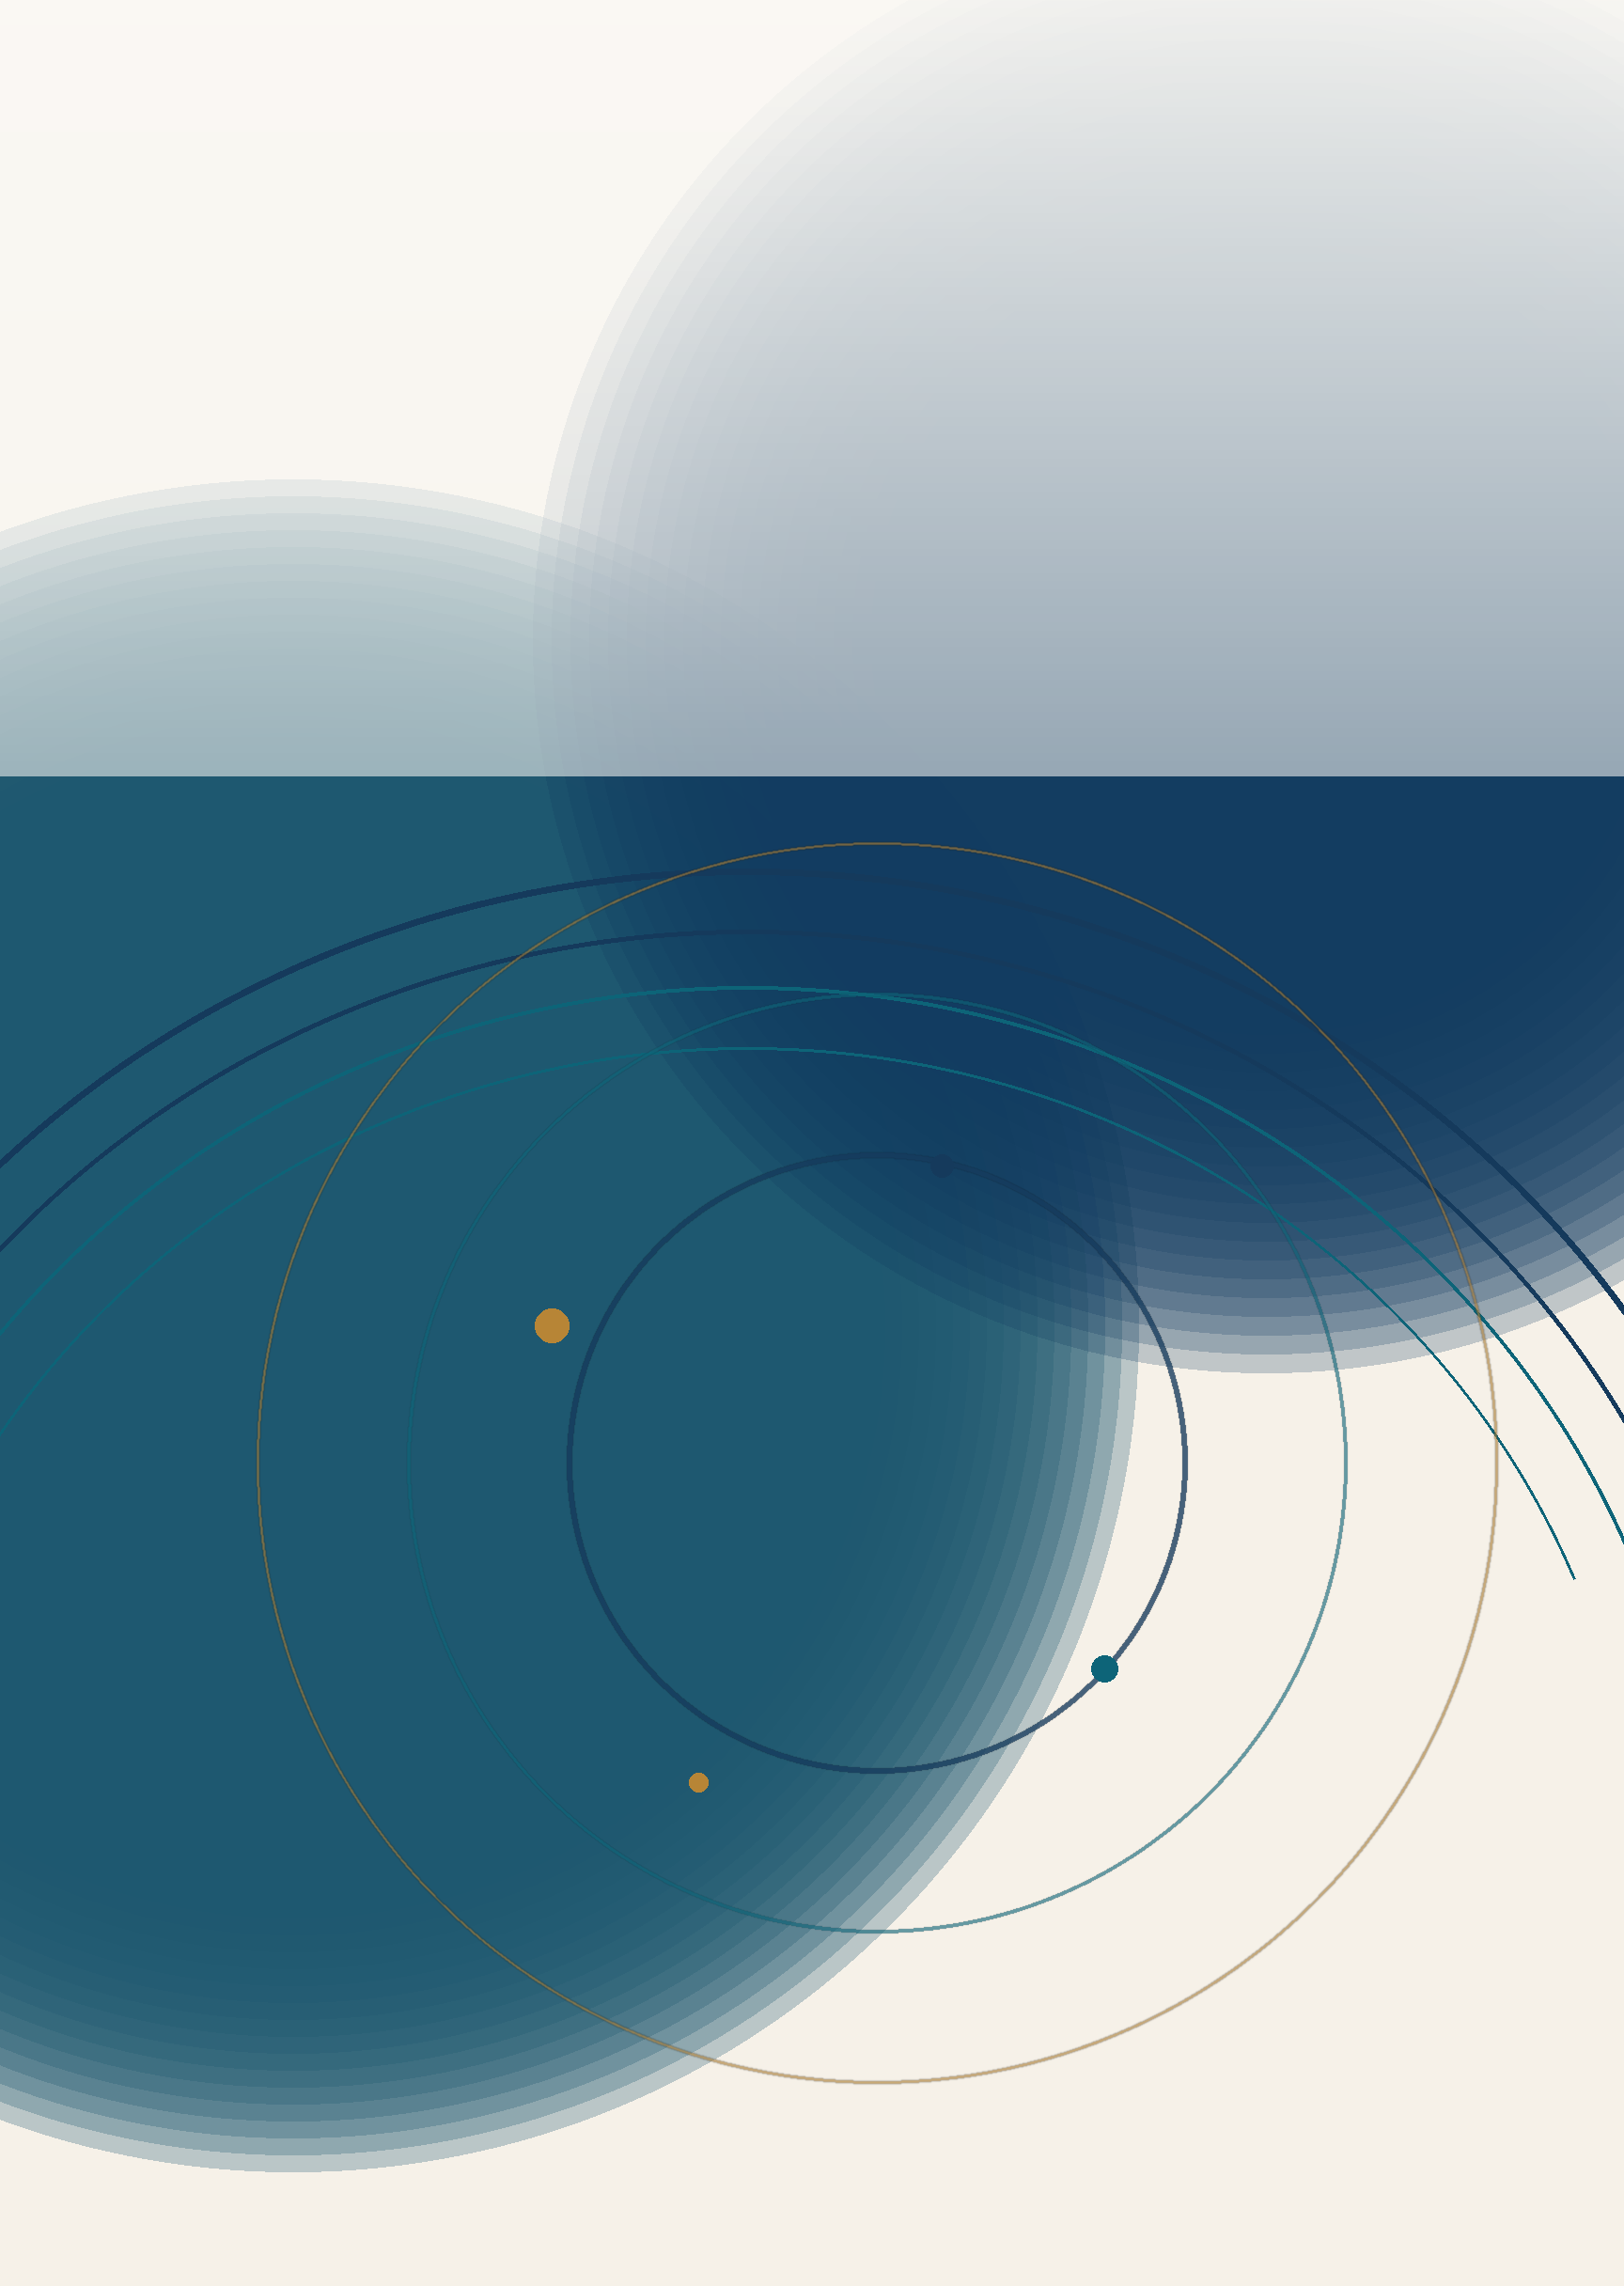
\includegraphics[height=\paperheight,keepaspectratio]{../../../generated_course_notes/core/cosmology/2009_winter_legacy_cosmology/assets/cover-art.png}%
  };
  \node[
    anchor=north west,
    align=left,
    text width=0.78\paperwidth,
    fill=white,
    fill opacity=0.9,
    rounded corners=8pt,
    inner xsep=10pt,
    inner ysep=8pt
  ] at ([xshift=0.08\paperwidth,yshift=-0.06\paperheight]current page.north west) {%
    {\fontsize{30}{33}\selectfont\bfseries\color{black!88} Kosmologie\\[0.85em]}
    {\large\color{black!72} Deutsche Ausgabe / Winter 2009, frühere Kosmologievorlesung}
  };
  \node[
    anchor=south west,
    align=left,
    text width=0.68\paperwidth,
    fill=white,
    fill opacity=0.82,
    text opacity=1,
    rounded corners=6pt,
    inner sep=12pt
  ] at ([xshift=0.08\paperwidth,yshift=0.08\paperheight]current page.south west) {%
    {\normalsize\color{black!78} Originalvorlesungen: Leonard Susskind\\[0.35em]}
    {\small\color{black!72} Begleitausgabe: \href{https://lazying.art}{LazyingArt LLC} / \href{https://github.com/lachlanchen/Video2Book}{Video2Book}}
  };
\end{tikzpicture}
\mbox{}
\end{titlepage}
\hypersetup{pageanchor=true}

\clearpage
\chapter{Über diese Notizen}
Diese unabhängig redigierten Begleitnotizen folgen den Vorlesungen von Leonard Susskind. Sie wurden anhand maschinell erstellter Transkripte, Untertitel und ausgewählter Tafelbilder rekonstruiert und anschließend mit dem verfügbaren Quellenmaterial abgeglichen. Sie sind kein Originalmanuskript von Professor Susskind und wurden von ihm weder geprüft noch gebilligt.

Diese Ausgabe wurde von \href{https://lazying.art}{LazyingArt LLC} mithilfe des Open-Source-Workflows \href{https://github.com/lachlanchen/Video2Book}{Video2Book} erstellt. Maschinell erstellte Transkripte sind separat verfügbar und können Erkennungsfehler enthalten. Redaktionelle Klarstellungen und nichttriviale Rekonstruktionen sind in Fußnoten gekennzeichnet.
\clearpage
\tableofcontents
\mainmatter
\chapter{Geometrie des expandierenden Universums}

Im Mittelpunkt stehen das expandierende Universum und seine Geometrie. Ziel ist es, zu beschreiben, was es bedeutet, dass sich der Raum ausdehnt, bevor wir fragen, wodurch diese Expansion angetrieben wird. Die Newtonsche \(F=ma\) Kosmologie kommt später; erst danach werden Geometrie und Dynamik zum vollständigen Friedmann--Robertson--Walker-Rahmen zusammengeführt.

\section{Mitbewegte Koordinaten auf einer expandierenden Geraden}

Beginnen wir mit dem einfachstmöglichen Beispiel: einem eindimensionalen Raum, nicht der Raumzeit. Stellen wir uns eine unendliche Gerade mit gleichmäßig darauf verteilten Galaxien vor. Die Koordinate \(x\) misst noch keinen physikalischen Abstand. Sie bezeichnet die Galaxien. Man kann \(x\) als Namen einer Galaxie auffassen; dieser Name bleibt der Galaxie zugeordnet, selbst wenn sich die gesamte Anordnung ausdehnt oder zusammenzieht.

Der physikalische Abstand zwischen der mit \(x=0\) bezeichneten Galaxie und der mit \(x=1\) bezeichneten Galaxie sei \(a\). Dann ist der physikalische Abstand zwischen beliebigen zwei Galaxien
\begin{equation}
d=a\,\Delta x.
\end{equation}
Die Koordinatendifferenz \(\Delta x\) ist lediglich die Differenz der Bezeichnungen. Der Faktor \(a\) wandelt diese Differenz in einen tatsächlichen, mit Maßstäben gemessenen Abstand um.

Stellen wir uns nun vor, die Gerade sei ein elastischer Faden, der gedehnt wird. Die Bezeichnungen bleiben den Galaxien zugeordnet, doch der Abstand zwischen benachbarten Galaxien ändert sich mit der Zeit. Dieselbe Beziehung lautet nun
\begin{equation}
d(t)=a(t)\,\Delta x.
\end{equation}
In diesem Stadium bedeutet Homogenität schlicht, dass benachbarte Galaxien überall gleich weit voneinander entfernt sind, auch wenn sich dieser gemeinsame Abstand mit der Zeit ändern kann.

\section{Das Hubble-Gesetz und das Fehlen eines Zentrums}

Um die Relativgeschwindigkeit zweier fest gewählter Galaxien zu bestimmen, halten wir das Galaxienpaar fest, sodass sich \(\Delta x\) nicht mit der Zeit ändert. Durch Differenzieren erhalten wir
\begin{align}
\dot d &= \dot a\,\Delta x \\
       &= \frac{\dot a}{a}\,a\,\Delta x \\
       &= \frac{\dot a}{a}\,d.
\end{align}
Definieren wir
\begin{equation}
H(t)\equiv \frac{\dot a}{a},
\end{equation}
dann gilt
\begin{equation}
\dot d = H(t)\,d.
\end{equation}
Das ist das Hubble-Gesetz.

Die historische Bezeichnung ``Hubble-Konstante'' ist irreführend. Die Größe ist im Raum konstant, nicht in der Zeit. Zu einem gegebenen Zeitpunkt hat sie für alle Galaxien denselben Wert, ändert sich aber im Allgemeinen im Lauf der Entwicklung des Universums. Treffender ist die Bezeichnung Hubble-Parameter.

Das Gesetz besagt, dass weiter entfernte Galaxien sich schneller entfernen. Es zeichnet kein Zentrum aus. In der Argumentation wird weder \(x=0\) noch irgendein anderer Punkt besonders hervorgehoben. Jeder Beobachter sieht dieselbe Gesetzmäßigkeit. Das expandierende Universum dieses Modells ist daher keine Explosion an einem ausgezeichneten Ort.

Die Rotverschiebung kommt unmittelbar ins Spiel. Tauschen zwei Galaxien, die sich voneinander entfernen, Lichtsignale aus, so ist das empfangene Licht rotverschoben. Je größer die Fluchtgeschwindigkeit, desto größer die Rotverschiebung. Spektrallinien geben uns daher Aufschluss über Fluchtgeschwindigkeiten. Abstände sind schwieriger zu messen, und Hubbles frühe Schätzungen waren grob. Sein erstes Diagramm ergab keine perfekte Gerade, sondern eine verstreute Punktwolke mit großen Unsicherheiten. Dennoch hielt das geometrische Prinzip dem Rauschen stand: Die Fluchtgeschwindigkeit ist proportional zum Abstand.

\begin{classroomqa}
\audiencequestion{Bewegen sich weit genug voneinander entfernte Galaxien nach dem Hubble-Gesetz schneller als mit Lichtgeschwindigkeit?}\lecturetimestamp{00:20:23}
\lecturerresponse{Ja, in diesem Sinne der Flucht tun sie das. Was Sie sagen, ist richtig. Darauf kommen wir ganz bestimmt noch zurück. Das ist eine der wichtigsten Fragen.}
\end{classroomqa}

\section{Höhere Dimensionen, Isotropie und die Zeitabhängigkeit von \(a(t)\)}

Wenn weitere räumliche Dimensionen hinzukommen, ändert sich nichts Wesentliches. In zwei Dimensionen stellen wir uns ein quadratisches Gitter von Galaxien vor, bezeichnet durch \((x,y)\), in drei Dimensionen eines mit Bezeichnungen \((x,y,z)\). Auch diese Koordinaten sind mitbewegte Bezeichnungen. Sie bewegen sich mit den Galaxien, statt den physikalischen Abstand direkt zu messen.

Warum sollte der Abstand in \(x\)-Richtung derselbe sein wie in \(y\)-Richtung? Die Antwort ist eine Beobachtungsfrage. Wären Galaxien in einer Richtung systematisch dichter gedrängt als in einer anderen, sähe der Himmel in verschiedene Richtungen unterschiedlich aus. Auf hinreichend großen Skalen ist das nicht der Fall. Diese Richtungsunabhängigkeit ist Isotropie.

In zwei Dimensionen beträgt der Abstand zwischen zwei Galaxien
\begin{equation}
d=a\sqrt{(\Delta x)^2+(\Delta y)^2},
\end{equation}
und in drei Dimensionen
\begin{equation}
d=a\sqrt{(\Delta x)^2+(\Delta y)^2+(\Delta z)^2}.
\end{equation}
Für ein festes Galaxienpaar bleiben die Koordinatendifferenzen konstant. Erneutes Differenzieren ergibt daher
\begin{equation}
\dot d=\frac{\dot a}{a}\,d.
\end{equation}
Das Hubble-Gesetz bleibt unverändert.

Homogenität bedeutet Gleichheit von Ort zu Ort. Isotropie bedeutet Gleichheit in allen Richtungen. Auf kleinen Skalen gilt keines von beidem exakt. Ein Blick durch die Milchstraße unterscheidet sich von einem Blick senkrecht zu ihrer Ebene, und einzelne Galaxien sind auf kurzen Abständen nicht gleichmäßig verteilt. Mittelt man jedoch über viele Galaxien, erscheint das Universum auf großen Skalen näherungsweise überall und in jeder Richtung gleich.

\begin{classroomqa}
\audiencequestion{Wenn die Geschwindigkeit proportional zum Abstand ist und der Abstand zunimmt, muss sich dann ein festes Galaxienpaar immer schneller voneinander entfernen?}\lecturetimestamp{00:40:22}
\lecturerresponse{Nein. Das Hubble-Gesetz besagt, dass die Fluchtgeschwindigkeit zu einem gegebenen Zeitpunkt proportional zum Abstand ist. Für sich genommen sagt es nicht aus, ob die Geschwindigkeit eines festen Galaxienpaars im Lauf der Zeit zunimmt oder abnimmt. Das hängt von der genauen Zeitabhängigkeit von \(a(t)\) ab. Wenn \(a(t)\propto t\), entfernen sich benachbarte Galaxien mit konstanter Geschwindigkeit voneinander. Wenn \(a(t)\propto t^2\), nimmt die Fluchtgeschwindigkeit eines festen Paars mit der Zeit zu. Wenn \(a(t)\propto \log t\), nimmt sie mit der Zeit ab. Das Gesetz \(\dot d=(\dot a/a)d\) gilt als Funktion des Abstands immer; Beschleunigung und Verzögerung sind jedoch davon getrennte Fragen.}
\end{classroomqa}

Lange Zeit erwarteten Kosmologen, dass sich die Expansion des Universums verlangsamt, da die Gravitation eine anfängliche Expansion bremsen sollte, so wie sie einen nach oben geworfenen Körper abbremst. Hier geht es lediglich darum, dass das Hubble-Gesetz für sich genommen das Verhalten von \(\dot a\) oder \(\ddot a\) nicht festlegt.

\begin{classroomqa}
\audiencequestion{Wie legt man den Anfangswert des Skalenfaktors \(a\) fest?}\lecturetimestamp{00:46:18}
\lecturerresponse{Seine Gesamtnormierung ist willkürlich. Physikalisch entscheidend ist nicht der Zahlenwert von \(a\) für sich genommen, sondern wie er sich ändert. Definiert man einen anderen Skalenfaktor \(b=3a\), so gilt \(\dot b/b=\dot a/a\). Eine Reskalierung von \(a\) mit einer Konstanten ändert die Konvention oder die Einheiten, nicht aber den Hubble-Parameter.}
\end{classroomqa}

\section{Von der räumlichen Metrik zur Raumzeitmetrik}

Ersetzen wir nun \(\Delta x\) durch \(dx\). Der physikalische Abstand zwischen benachbarten Punkten ist
\begin{equation}
ds=a\,dx,
\end{equation}
also gilt
\begin{equation}
ds^2=a^2\,dx^2.
\end{equation}
Das ist die räumliche Metrik in einer Dimension. Der Koeffizient von \(dx^2\) ist
\begin{equation}
g_{xx}=a^2.
\end{equation}
Ein expandierendes Universum lässt sich somit dadurch beschreiben, dass der räumliche Teil der Metrik von der Zeit abhängt.

Um vom Raum zur Raumzeit überzugehen, verwenden wir das relativistische Linienelement. In einer räumlichen Dimension gilt
\begin{equation}
d\tau^2=dt^2-a^2(t)\,dx^2.
\end{equation}
Für einen mitbewegten Beobachter ist \(dx=0\), also \(d\tau=dt\). Die gewöhnliche kosmische Zeit ist die Eigenzeit, die von Uhren gemessen wird, welche sich mit den Galaxien bewegen.

Die Tafelzeichnung ist an dieser Stelle hilfreich, weil sie die mitbewegten Weltlinien, das Linienelement und die Metrikschreibweise zusammenführt.
\begin{figure}[H]
\centering
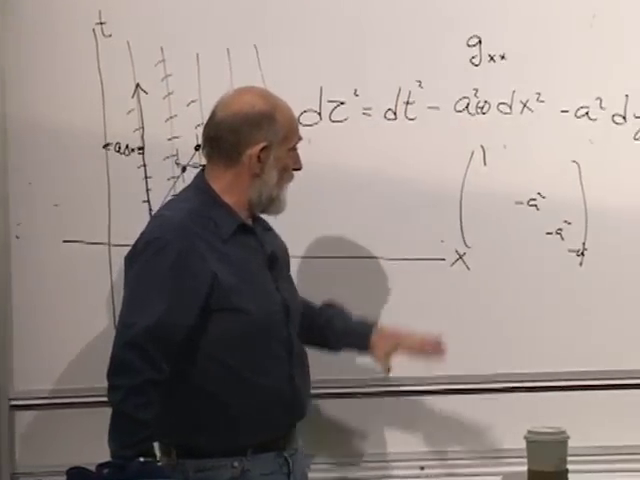
\includegraphics[width=0.82\textwidth]{lecture_01_figure_02.png}
\caption{Mitbewegte Weltlinien in einem expandierenden eindimensionalen Universum und das zugehörige Raumzeitintervall.}
\end{figure}

In drei räumlichen Dimensionen ergibt dasselbe Schema die vorsichtige Verallgemeinerung\footnote{Die Tafel ist teilweise verdeckt, und zwar im Bereich 00:56:38--00:58:51. Diese dreidimensionale Form folgt der mündlichen Verallgemeinerung von einer auf drei räumliche Dimensionen sowie dem sichtbaren diagonalen Muster auf der Tafel.}
\begin{equation}
d\tau^2=dt^2-a^2(t)\bigl(dx^2+dy^2+dz^2\bigr),
\end{equation}
mit der Diagonalmetrik
\begin{equation}
g_{\mu\nu}=\mathrm{diag}\bigl(1,-a^2,-a^2,-a^2\bigr).
\end{equation}
Die gemischten Terme verschwinden:
\begin{equation}
g_{tx}=g_{ty}=g_{tz}=0.
\end{equation}

Homogenität bedeutet, dass die Metrikkoeffizienten zwar von der Zeit, nicht aber vom Ort abhängen dürfen. Isotropie bedeutet, dass die drei räumlichen Richtungen auf dieselbe Weise eingehen.

\begin{classroomqa}
\audiencequestion{Sollen wir \(dx\) nicht als Abstand auffassen?}\lecturetimestamp{01:01:18}
\lecturerresponse{Nein. \(dx\) ist nicht der Abstand. \(a\,dx\) ist der Abstand. \(dx\) ist lediglich ein Koordinatenintervall. Man kann es sich so vorstellen: Zu einem bestimmten Zeitpunkt zeichnet jemand ein Koordinatennetz durch die Galaxien und sorgt dann dafür, dass das Netz ihnen folgt. Der Koordinatenabstand bleibt konstruktionsbedingt konstant, während sich der physikalische Abstand ändert. Man könnte die Längeneinheiten statt in \(a\) auch in \(x\) unterbringen; das ist eine Konvention. Entscheidend ist das Produkt \(a\,dx\).}
\end{classroomqa}

\begin{classroomqa}
\audiencequestion{Der Metrikkoeffizient von \(dt^2\) ist gleich \(1\). Ist auch das nur eine Konvention?}\lecturetimestamp{01:03:24}
\lecturerresponse{Ja. Für sich genommen steckt darin keine Physik. Hinge der Koeffizient nur von der Zeit ab, könnte man die Zeitvariable so ändern, dass er einfach \(dt^2\) wäre. Ebenso kann man Einheiten mit \(c=1\) wählen. Keine Konvention ist hier hingegen, dass der Koeffizient nicht vom Ort abhängt, auch wenn er von der Zeit abhängen kann.}
\end{classroomqa}

\begin{classroomqa}
\audiencequestion{Was ergibt sich für den Energie-Impuls-Tensor, wenn man dies in Einsteins Feldgleichungen einsetzt?}\lecturetimestamp{01:05:59}
\lecturerresponse{Das ist die nächste Art von Frage, gehört aber zur Dynamik und nicht zur gegenwärtigen Diskussion. Man kann diese Metrik in Einsteins Gleichungen einsetzen und fragen, welche Energie-Impuls-Verteilung sie zu einer Lösung machen würde. Das ist sehr wichtig, doch im Moment geht es um Geometrie, nicht um Dynamik.}
\end{classroomqa}

\section{Was der Horizont verbirgt}

Das Universum wird auf großen Skalen nur näherungsweise als homogen und isotrop behandelt. Auf der Skala von Sternen, Planeten oder auch einzelnen Galaxien ist es keineswegs homogen. Auch bei lokalen Beobachtungen ist es nicht exakt isotrop.

Ein Feld eines Bauern veranschaulicht die Abhängigkeit von der Skala. Auf einer Skala wirkt es regelmäßig; auf einer viel kleineren Skala ist das offensichtlich nicht der Fall; auf einer Skala, die größer ist als das ganze Feld, wirkt es wiederum nicht mehr homogen. In der Kosmologie ist es ähnlich. Mittelt man über viele Galaxien, erscheint die Verteilung auf großen Skalen ungefähr gleichmäßig. Auf hinreichend kleinen Skalen ist sie es nicht.

Das Universum ist größer als der Teil, den wir sehen können, und größer als der Teil, den wir jemals sehen können. Auf den Skalen, die tatsächlich beobachtbar sind, ist es abgesehen von lokalen Schwankungen isotrop und homogen. Jenseits davon gibt es keine unmittelbare Beobachtungsgarantie.

\begin{classroomqa}
\audiencequestion{Sie sagten, wir würden es nie wirklich direkt herausfinden. Heißt das, dass es vielleicht einen indirekten Weg gibt, es herauszufinden?}\lecturetimestamp{01:10:34}
\lecturerresponse{Vielleicht. Heute geht man meist davon aus, dass das Universum auf hinreichend großen Skalen nicht homogen ist, und ich selbst vermute das auch. Doch diese Vermutung kann ich weder bestätigt bekommen noch widerlegt sehen, denn aus grundlegenden Gründen werden wir nicht viel weiter blicken können als heute. Das liegt an der Existenz eines Horizonts.}
\end{classroomqa}

\begin{classroomqa}
\audiencequestion{Könnte man nicht die Gravitation nutzen, um nach Massen jenseits dessen zu suchen, was man sehen kann?}\lecturetimestamp{01:11:53}
\lecturerresponse{Nein. Eine weit entfernte Masse kann uns einfach in den freien Fall versetzen. In einem geschlossenen Raum befinden wir uns im Gravitationsfeld der Sonne und umkreisen sie. Doch ohne nach draußen zu sehen, gibt es keine einfache Möglichkeit zu erkennen, dass die Sonne da ist. Nur Gezeitenkräfte verraten es; ist die Quelle weit genug entfernt, können diese Gezeiteneffekte zu klein sein, um nachweisbar zu sein.}
\end{classroomqa}

Der Horizont ist somit eine unüberwindbare Grenze für unmittelbare Erkenntnis. Er sagt sogar mit praktisch völliger Gewissheit, dass das Universum ein mindestens tausendmal größeres Volumen hat als der Bereich, den wir jemals sehen können, und verschiebt die Begründung dieser Behauptung auf später.

\section{Begrenzt, aber ohne Rand}

Wenden wir uns nun geschlossenen Geometrien zu. Die unendliche Gerade ist offen und unbegrenzt. Eine Strecke ist insofern begrenzt, als sie nur eine endliche Ausdehnung hat. Begrenzt bedeutet nicht, dass es einen Rand gibt, sondern dass die Ausdehnung endlich ist.

Ein Würfel mit Wänden eignet sich nicht. Er verletzt die Homogenität, denn jemand in Wandnähe ist nicht gleichwertig mit jemandem weit von einer Wand entfernt. Zudem verletzt er die Isotropie, denn selbst jemand im Zentrum sieht in verschiedene Richtungen Unterschiedliches.

Auch das Innere eines Kreises oder einer Kugel eignet sich nicht. Jemand im Zentrum sieht in alle Richtungen dasselbe, doch diese Symmetrie gilt nur für einen einzigen ausgezeichneten Punkt. Bewegt man sich vom Zentrum weg, ist die Wand in einer Richtung nah und in einer anderen weit entfernt. Für beliebige Beobachter ist der Raum dann weder homogen noch isotrop.

Auf sehr großen Skalen lautet die Arbeitshypothese, dass das Universum homogen und isotrop ist. Das ist das kosmologische Prinzip. Es ist nützlich, aber nicht vor Revision geschützt.

\begin{classroomqa}
\audiencequestion{Folgt aus Isotropie überall auch Homogenität?}\lecturetimestamp{01:18:57}
\lecturerresponse{Ja. Wenn jeder Beobachter in alle Richtungen dasselbe sieht, folgt daraus Homogenität. Die Umkehrung gilt jedoch nicht. Homogenität allein bedeutet nicht Isotropie. Ein Universum kann homogen sein und dennoch eine ausgezeichnete Richtung haben, etwa wenn es von Pfeilen erfüllt wäre, die alle in dieselbe Richtung zeigen.}
\end{classroomqa}

Das passende begrenzte Modell ist die Oberfläche einer strukturfreien Kugel. Ein zweidimensionales Wesen, das auf diese Oberfläche beschränkt ist, findet jeden Ort lokal wie jeden anderen und jede Richtung wie jede andere, obwohl seine Welt endlich ist. Sie ist begrenzt, aber ohne Rand.

\section{Ein geschlossenes eindimensionales Universum auf einem Kreis}

Um die Algebra einfach zu halten, reduzieren wir das Kugelbeispiel auf eine räumliche Dimension: Leben auf einem Kreis. In einer Dimension bedeutet Isotropie, dass links und rechts gleichwertig sind. Ein Kreis weist genau diese Eigenschaft auf. Wir wählen einen Punkt und nennen ihn \(\theta=0\). Jeder andere Punkt wird durch eine Winkelkoordinate \(\theta\) bezeichnet, gemessen im Bogenmaß. Ein Punkt unmittelbar auf einer Seite des Ursprungs lässt sich entweder durch einen kleinen negativen Winkel oder durch einen Winkel knapp unter \(2\pi\) beschreiben. Diese Periodizität gehört zur Geometrie.

Den Bewohnern des Kreises steht der Umfang zur Verfügung, nicht aber ein äußerer Radius oder ein Zentrum. Sie können die gesamte Strecke ringsum messen, indem sie am Kreis entlanggehen, bis sie zum selben Punkt zurückkehren. Zeichnet man den Kreis in einer umgebenden Ebene, kann man auch eine radiusähnliche Größe einführen. Sie gehört jedoch zur Einbettung und nicht zu der intrinsischen Geometrie, die die Bewohner messen.

Die Tafelzeichnung ist hier hilfreich, weil sie die Winkelbezeichnungen und den Gesamtumfang in derselben Darstellung zeigt.
\begin{figure}[H]
\centering
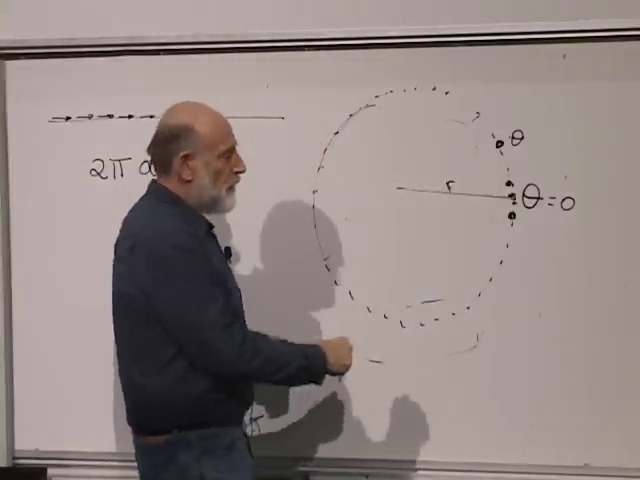
\includegraphics[width=0.82\textwidth]{lecture_01_figure_03.png}
\caption{Winkeldarstellung eines geschlossenen eindimensionalen Universums mit dem Gesamtumfang \(2\pi a\).}
\end{figure}

Eine praktische Konvention lautet\footnote{Zwischen 01:26:40--01:29:20 wechselt die Schreibweise kurz zwischen dem Gesamtumfang selbst als Skalenfaktor und der Darstellung als \(2\pi a\). Hier verwenden wir die spätere Konvention, weil sie in die Formel für die Bogenlänge übernommen wird.}
\begin{equation}
L=2\pi a,
\end{equation}
wobei \(L\) der Gesamtumfang ist.

Für einen kleinen Winkelabstand \(\Delta\theta\) ist der physikalische Abstand
\begin{equation}
d=a\,\Delta\theta.
\end{equation}
Im Grenzfall infinitesimaler Abstände erhalten wir
\begin{equation}
ds=a\,d\theta,
\end{equation}
und somit
\begin{equation}
ds^2=a^2\,d\theta^2.
\end{equation}
Das ist die lokale Metrik auf dem Kreis.

Hängt \(a\) von der Zeit ab, expandiert oder kontrahiert das geschlossene eindimensionale Universum. Für ein festes Galaxienpaar gilt
\begin{equation}
d(t)=a(t)\,\Delta\theta,
\end{equation}
also
\begin{equation}
\dot d=\dot a\,\Delta\theta
      =\frac{\dot a}{a}\,d.
\end{equation}
Auch hier gilt das Hubble-Gesetz, zumindest für Galaxienpaare, die nicht so weit voneinander entfernt sind, dass die andere Richtung um den Kreis herum mehrdeutig wird.

Die Raumzeitmetrik lautet dann
\begin{equation}
d\tau^2=dt^2-a^2(t)\,d\theta^2.
\end{equation}
Ist \(a\) konstant, ist das Raumzeitbild ein Zylinder. Gilt \(a\propto t\), ist es ein Kegel. Ändert sich \(a(t)\) unregelmäßiger, wird das Bild vasenförmig.

Lässt man das Bild rückwärts ablaufen, kommen sich die Galaxien immer näher. Gäbe es \(360\) Galaxien auf dem Kreis, wären sie zu späten Zeiten weit voneinander entfernt, zu früheren Zeiten sehr dicht beieinander und noch früher dichter zusammengedrängt. Schließlich wären sie keine getrennten Galaxien mehr und noch früher nicht einmal getrennte Atome. Dennoch gibt es weiterhin keinen ausgezeichneten Punkt im Raum.

Das ist die klarste Antwort auf die Frage, wo der Urknall in diesem Modell stattgefunden hat. Wenn \(a(t)\to 0\), geht jeder Abstand \(a(t)\,\Delta\theta\) gegen null. Das gesamte Universum schrumpft überall gleichzeitig. Die Galaxien fliegen nicht von einem ausgezeichneten Ort in einem äußeren Raum fort. Vielmehr ändert die Geometrie selbst ihren Maßstab. In diesem Sinn lautet die Antwort: überall.

\begin{classroomqa}
\audiencequestion{Sie sagten, die Raumzeit sei gekrümmt. Wäre sie auch gekrümmt, wenn sie ein Zylinder wäre?}\lecturetimestamp{01:38:04}
\lecturerresponse{Nein. Wäre sie ein Zylinder, wäre sie nicht gekrümmt. Das ist der Fall, in dem \(a\) zeitlich konstant ist. Gekrümmt wirkt der Zylinder nur, weil er in einem höherdimensionalen Raum gezeichnet wird. Schneidet man ihn auf, lässt er sich ohne Dehnung flach ausbreiten.}
\end{classroomqa}

Von dort führt die Diskussion zum Kegel. Wenn \(a\propto t\), ist das Raumzeitbild ein Kegel. Abseits seiner Spitze ist auch der Kegel im selben intrinsischen Sinn flach: Er lässt sich zu einer Ebene aufklappen. Die Spitze ist anders. Sie ist eine Kegelsingularität.

Als Nächstes folgen die Geometrie des sphärischen Universums und dann die Dynamik, die bestimmt, wie \(a(t)\) wächst oder schrumpft.

\chapter{Newtonsche Kosmologie und die Friedmann-Gleichung}

Letztes Mal haben wir über die Metrik des Raums gesprochen. Als Nächstes geht es um die Dynamik: Wie ändert sich der Skalenfaktor mit der Zeit? Zunächst betrachten wir ein wenig Geometrie und anschließend die Newtonsche Kosmologie. Die Friedmann-Gleichung wird hier noch nicht aus der allgemeinen Relativitätstheorie hergeleitet, sondern aus den Newtonschen Gleichungen.

\section{Homogenität, Isotropie und eine zeitabhängige Metrik}

Homogenität und Isotropie sind die grundlegenden Annahmen. Ist das Universum homogen und isotrop und verändert es sich mit der Zeit, dann gilt das Hubble-Gesetz stets. Zu jedem festgelegten Zeitpunkt ist die Fluchtgeschwindigkeit proportional zur Entfernung,
\begin{equation}
v = H(t)\,d.
\end{equation}
und zwar linear. Nicht die Zeit, sondern der Raum ist hier maßgeblich: Zu einem gegebenen Zeitpunkt gilt überall derselbe Proportionalitätsfaktor.

\begin{classroomqa}
\audiencequestion{Heißt das, dass die Proportionalität linear ist?}\lecturetimestamp{00:02:06}
\lecturerresponse{Ja. Zu einem festen Zeitpunkt ist die Fluchtgeschwindigkeit linear proportional zur Entfernung. Der Proportionalitätsfaktor ist die Hubble-Konstante. Im Allgemeinen hängt sie von der Zeit ab, variiert aber nicht von Ort zu Ort im Raum.}
\end{classroomqa}

Deshalb ist die Bezeichnung ``Hubble-Konstante'' irreführend. Sie ist bezüglich des Ortes im Raum konstant, nicht aber bezüglich der Zeit.

Eine naheliegende Frage lautet nun: Wenn sich der Raum ausdehnt, warum dehnen sich dann Meterstäbe nicht ebenfalls aus? Die Antwort lautet, dass Meterstäbe durch Kräfte zusammengehalten werden, die sehr viel stärker sind als alles, was mit der kosmologischen Expansion auf atomaren Skalen zusammenhängt. Gebundene Objekte bleiben gebunden. Was sich ausdehnt, ist der Abstand zwischen hinreichend voneinander getrennten Dingen, etwa zwischen Galaxien, die so weit auseinanderliegen, dass sie einander nicht stark zusammenhalten.

\begin{classroomqa}
\audiencequestion{Gibt es ein Problem damit, dass sich die Messstäbe ebenfalls ausdehnen?}\lecturetimestamp{00:04:00}
\lecturerresponse{Nein. Die Messstäbe dehnen sich nicht aus. Die Koordinaten dehnen sich aus. Die Kräfte, die Meterstäbe zusammenhalten, sind viel stärker als die Auswirkungen der Expansion. Daher dehnen sich gewöhnliche gebundene Objekte nicht mit dem Hintergrund aus. Galaxien, die weit genug voneinander entfernt sind, entfernen sich voneinander, Meterstäbe jedoch nicht.}
\end{classroomqa}

Man kann sich sogar einen winzigen zusätzlichen abstoßenden Effekt zwischen Atomen vorstellen. Auch der würde einen Stab nicht auseinanderreißen. Er würde lediglich den Gleichgewichtsabstand ein wenig verschieben, so wie eine kleine zusätzliche Kraft die Gleichgewichtslage einer steifen Feder verändert.

\begin{classroomqa}
\audiencequestion{Man kann es aber nicht als Kraft zwischen Punkten modellieren, stimmt das? Denn sonst wäre es eine Beschleunigung.}\lecturetimestamp{00:05:29}
\lecturerresponse{Eine kleine zusätzliche Kraft zwischen Atomen kann man sich vorstellen. Ist sie jedoch winzig im Vergleich zu den Bindungskräften, verschiebt sie nur geringfügig die Gleichgewichtslage. Die Expansion allein erzeugt kein gewöhnliches Kraftgesetz. Manche Arten der Expansion lassen sich durch eine Kraft modellieren, nämlich die beschleunigte Expansion; das ist aber eine Frage für später.}
\end{classroomqa}

Nützlich sind also Koordinaten, die in die expandierende Materieverteilung eingebettet sind. Galaxien ohne zusätzliche Pekuliarbewegung behalten dieselben Koordinatenwerte. Was sich mit der Zeit ändert, ist die Beziehung zwischen dem Koordinatenabstand und dem in Metern gemessenen physikalischen Abstand. Diese Beziehung wird durch den Skalenfaktor \(a(t)\) beschrieben.

Für einen flachen Raum lässt sich die räumliche Metrik schreiben als
\begin{equation}
ds^2 = a(t)^2\left(dx^2+dy^2+dz^2\right).
\end{equation}
Hier ist \(a\) der tatsächliche, in Metern gemessene Abstand zwischen benachbarten Punkten, die im Koordinatenraum eine Einheit voneinander entfernt sind. Dehnt sich das Universum aus, wird \(a\) zeitabhängig.

Um zur Raumzeit überzugehen, geht man von der speziell-relativistischen Form
\begin{equation}
d\tau^2 = dt^2 - ds^2,
\end{equation}
aus und setzt die räumliche Metrik ein. Das ergibt
\begin{equation}
d\tau^2 = dt^2 - a(t)^2\left(dx^2+dy^2+dz^2\right).
\end{equation}
Die Koeffizienten hängen nicht vom Ort im Raum ab, sondern nur von der Zeit. In der Sprache der Metrik ist das die Aussage der Homogenität. Die Diagonalmetrik hat die Form
\begin{equation}
g_{\mu\nu}=\mathrm{diag}\!\left(1,-a(t)^2,-a(t)^2,-a(t)^2\right).
\end{equation}
\editorialnote{Die hier angegebene vollständige Diagonalmatrix entspricht der mündlichen Beschreibung des Metriktensors um 00:14:33. Der Tafelrahmen zeigt das Linienelement deutlich, aber keine vollständig lesbare Matrix.}

Es gibt keine Nebendiagonaleinträge: weder \(dx\,dy\) noch \(dx\,dt\) noch andere gemischte Terme. Die Metrik ist fast so einfach wie die der flachen Raumzeit. Das Besondere ist, dass die Beziehung zwischen räumlichem Maß und Zeit selbst zeitabhängig ist.

\begin{figure}
\centering
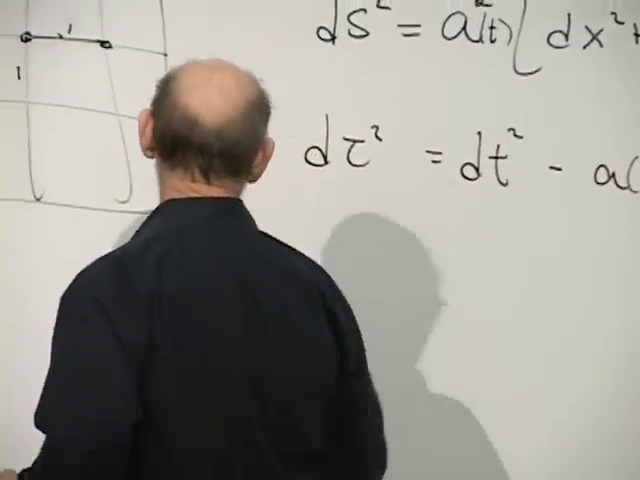
\includegraphics[width=0.62\textwidth]{lecture_02_figure_02.png}
\caption{Skizze eines mitbewegten Koordinatengitters und Raumzeitintervall mit zeitabhängigem Skalenfaktor.}
\end{figure}

Die Skizze verdeutlicht den entscheidenden Punkt. Alice und Bob bleiben in den mitbewegten Koordinaten eine Einheit voneinander entfernt, doch diese Koordinateneinheit entspricht mit der Zeit immer mehr Metern. Wäre \(a(t)\) zu einem Zeitpunkt in der Vergangenheit null gewesen, dann wären alle physikalischen Abstände null. Alles wäre zu einem einzigen Punkt zusammengedrängt. Deshalb entspricht \(a\to 0\) unendlicher Dichte. Wenn \(a\) wächst, wird das Universum immer diffuser.

Diese Form der Metrik gilt nicht in jedem Bezugssystem. Sie ist die Form im mit den Galaxien mitbewegten Bezugssystem.

\begin{classroomqa}
\audiencequestion{In dieser Gleichung: Die kleine Größe \(t\), \(a(t)\), wessen \(t\) ist das?}\lecturetimestamp{00:19:19}
\lecturerresponse{Das ist die Zeit, die von Uhren gemessen wird, die sich mit den Galaxien bewegen. Man stelle sich identische Uhren vor, die in derselben kosmischen Uhrenfabrik hergestellt und von den Galaxien mitgeführt werden. In diesem Bezugssystem entspricht die Zeitvariable genau dem, was diese Uhren messen. Entlang einer Galaxienweltlinie ist die Eigenzeit gleich dieser Koordinatenzeit.}
\end{classroomqa}

Tatsächlich gilt entlang der Weltlinie einer mitbewegten Galaxie
\begin{equation}
dx=dy=dz=0,
\end{equation}
also
\begin{equation}
d\tau^2 = dt^2,
\end{equation}
und damit
\begin{equation}
dt=d\tau.
\end{equation}

\begin{classroomqa}
\audiencequestion{Gibt es Transformationen, unter denen diese Form der Metrik invariant bleibt?}\lecturetimestamp{00:23:08}
\lecturerresponse{Ja, Rotationen, denn \(dx^2+dy^2+dz^2\) ist unter Rotationen invariant. Lorentz-Boosts erhalten diese Form dagegen nicht. Die Materie selbst zeichnet das mit den Galaxien mitbewegte Bezugssystem aus; in einem anderen Bezugssystem würde die Welt nicht isotrop erscheinen.}
\end{classroomqa}

\section{Ein Projektil in einem Gravitationsfeld}

Bevor wir die Newtonsche Mechanik auf das gesamte Universum anwenden, betrachten wir zunächst ein einfacheres Problem: eine große Masse \(M\), eine viel kleinere Masse \(m\) und einen anfänglichen Impuls nach außen. Nach diesem Impuls bewegt sich die kleine Masse einfach im Gravitationsfeld und verhält sich so, wie es Newtons Gesetze vorgeben.

Für die kosmologische Diskussion ist nicht das vollständige Bahnproblem entscheidend, sondern die Energieerhaltung. Die kinetische Energie lautet
\begin{equation}
\frac{1}{2}mv^2.
\end{equation}

\begin{figure}
\centering
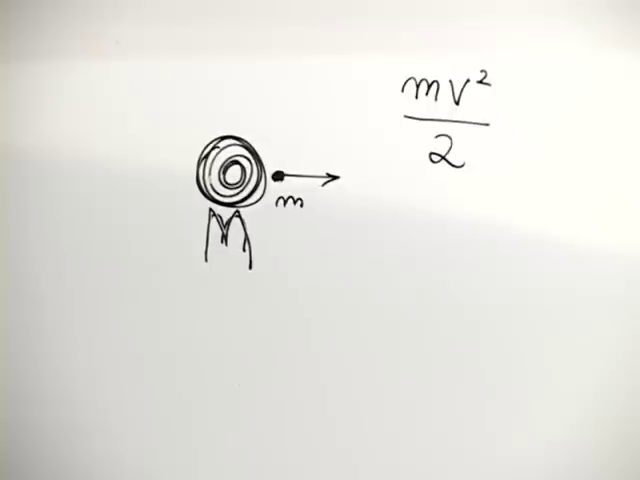
\includegraphics[width=0.42\textwidth]{lecture_02_figure_03.png}
\caption{Nach außen bewegte Testmasse und der Term für die kinetische Energie \(\frac{1}{2}mv^2\).}
\end{figure}

Die potenzielle Energie im Gravitationsfeld enthält das Produkt der Massen und der Newtonschen Gravitationskonstante; im Nenner steht eine Potenz des Abstands. Auf der Tafel stehen die Faktoren in der Reihenfolge \(mMG/D\), daher behalten wir diese Reihenfolge bei:
\begin{equation}
-\frac{mMG}{D}.
\end{equation}
Die Gesamtenergie ist somit
\begin{equation}
\frac{1}{2}mv^2-\frac{mMG}{D}.
\end{equation}
Die Energieerhaltung besagt lediglich, dass sich diese Größe für das betrachtete Teilchen nicht mit der Zeit ändert. Verschiedene Teilchen können unterschiedliche Energien haben.

\begin{figure}
\centering
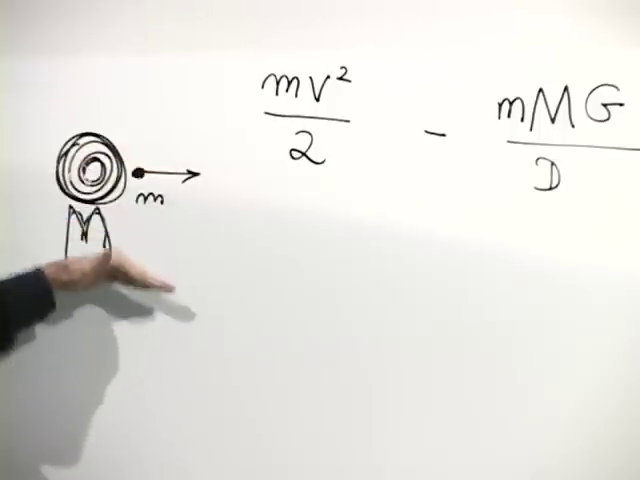
\includegraphics[width=0.62\textwidth]{lecture_02_figure_04.png}
\caption{Gesamte Newtonsche Energie einer radial bewegten Testmasse: kinetischer Term minus Gravitationspotenzial.}
\end{figure}

Das Minuszeichen ist entscheidend. Die potenzielle Energie im Gravitationsfeld ist negativ, weil die Gravitation anziehend wirkt. Nähert man das Teilchen an, nimmt die negative potenzielle Energie dem Betrag nach zu. Entfernt es sich, wird die potenzielle Energie weniger negativ.

\begin{classroomqa}
\audiencequestion{Nimmt die potenzielle Energie mit dem Abstand zu, statt abzunehmen?}\lecturetimestamp{00:34:13}
\lecturerresponse{Ja. Lassen wir die Konstanten außer Acht und betrachten die Graphen von \(1/D\) und \(-1/D\). Eine Kraft treibt das Teilchen in Richtung abnehmender potenzieller Energie. Eine anziehende Kraft entspricht daher der umgekehrten Kurve \(-1/D\): Die potenzielle Energie nimmt mit dem Abstand zu und wird negativer, wenn sich das Teilchen nach innen bewegt.}
\end{classroomqa}

\begin{figure}
\centering
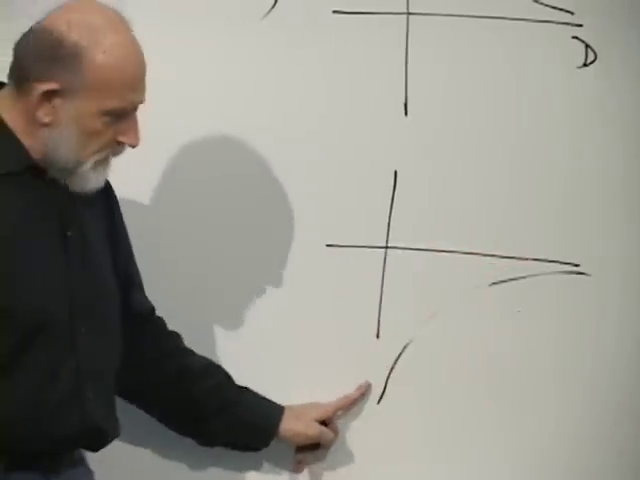
\includegraphics[width=0.46\textwidth]{lecture_02_figure_05.png}
\caption{Qualitativer Vergleich von \(1/D\) und \(-1/D\) zur Veranschaulichung des Vorzeichens der potenziellen Gravitationsenergie.}
\end{figure}

\section{Fluchtgeschwindigkeit}

Betrachten wir nun die möglichen Fälle. Die Energie kann positiv, negativ oder null sein. Andere Möglichkeiten gibt es nicht.

\begin{itemize}
\item Ist die Energie negativ, ist das Teilchen gebunden. Wirft man es mit zu geringer Geschwindigkeit nach oben, steigt es zunächst auf, wird langsamer, kehrt um und fällt zurück.
\item Ist die Energie positiv, entkommt das Teilchen. Die Gravitation bremst es zunächst ab, aber nicht genug, um es anzuhalten. Schließlich bewegt es sich mit einer asymptotisch nicht verschwindenden Geschwindigkeit nach außen.
\item Ist die Energie genau null, hat das Teilchen die Fluchtgeschwindigkeit. Das ist der Grenzfall zwischen Entkommen und Nichtentkommen.
\end{itemize}

Bei hinreichend kleiner Anfangsgeschwindigkeit dominiert von Anfang an der Potenzialterm, und die Energie ist negativ.

\begin{figure}
\centering
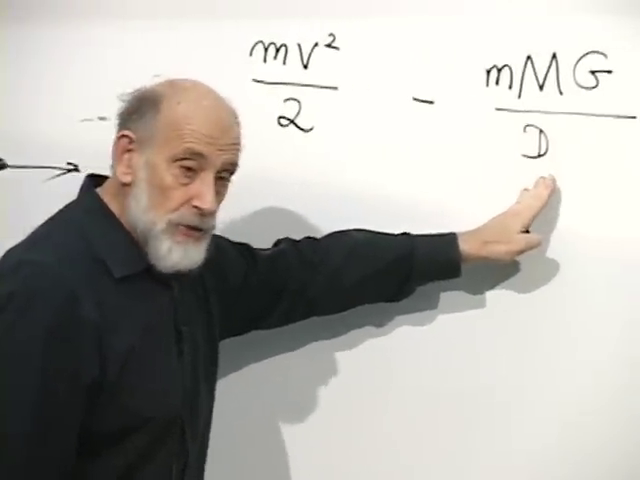
\includegraphics[width=0.62\textwidth]{lecture_02_figure_06.png}
\caption{Bei geringer Geschwindigkeit nach außen dominiert der negative Potenzialterm die Gesamtenergie.}
\end{figure}

Im Fall verschwindender Energie nimmt der Abstand weiterhin zu, während die Geschwindigkeit immer weiter abnimmt. Das Teilchen kann zu keiner endlichen Zeit zur Ruhe kommen. Denn dann würde es zurückfallen. Der Abstand ist also unbeschränkt, während die Geschwindigkeit gegen null geht.

Genau diese Analogie ist für die Kosmologie wichtig. Das Universum kann sich genauso verhalten. Ist die anfängliche Hubble-Expansion nach außen stark genug, entkommt alles allem anderen. Ist sie zu gering, setzt sich die Gravitation durch, und es kommt zu einem gewaltigen Kollaps. Dazwischen liegt der Grenzfall, der genau der Fluchtgeschwindigkeit entspricht.

\section{Newtonscher Satz}

Die kosmologische Vereinfachung beruht auf dem Newtonschen Satz für das inverse-quadratische Kraftgesetz.

Ist Materie kugelsymmetrisch um ein Zentrum verteilt, dann ist die Gravitationskraft auf ein Teilchen außerhalb der Verteilung genau dieselbe, als wäre die gesamte Masse im Zentrum konzentriert. Der Satz geht jedoch noch weiter: Befindet sich das Teilchen innerhalb der Verteilung, trägt nur die Masse innerhalb seines Radius bei. Die weiter außen liegende Masse übt insgesamt keine Kraft aus.

Die anschaulichste Fassung des Satzes betrifft eine dünne Kugelschale. Eine ideale Kugelschale übt auf ein Teilchen an jeder Stelle im Inneren keine Gravitationskraft aus, auch nicht abseits des Zentrums. Das mag zunächst überraschend sein, gilt aber für das Kraftgesetz \(1/r^2\).

\begin{classroomqa}
\audiencequestion{Bei dem Beispiel, das Sie gerade gegeben haben: Sollte es uns nicht ein wenig überraschen, dass die Kraft beim Überqueren der Grenze durch das Teilchen offenbar unstetig ist?}\lecturetimestamp{00:48:19}
\lecturerresponse{Ja. Bei einer idealen, unendlich dünnen Schale ist das überraschend und eine Besonderheit des Kraftgesetzes \(1/r^2\). Eine reale Schale hat eine Dicke, wodurch sich die Änderung glättet. Die scharfe Aussage für eine ideale Schale ist jedoch genau die bemerkenswerte Eigenschaft des Newtonschen Satzes.}
\end{classroomqa}

Eine anschauliche Analogie macht den Satz plausibel. Ersetzen wir eine Punktmasse durch eine punktförmige Wasserquelle. In drei Dimensionen nimmt die nach außen gerichtete Strömung wie \(1/r^2\) ab. Ordnet man solche Quellen lückenlos rings um eine Kugelschale an, sieht die Strömung außerhalb der Schale genauso aus, als wäre alles im Zentrum konzentriert. Innerhalb der Schale kann es keine Nettoströmung geben, denn im Zentrum befindet sich keine Quelle. Dieselbe Struktur liegt dem Gravitationssatz zugrunde.

Es geht hier nicht darum, den Satz erneut herzuleiten, sondern ihn anzuwenden.

\section{Ein homogenes Universum als Zweikörperproblem}

Kehren wir nun zur Kosmologie zurück. Betrachten wir einen kleinen Bereich des Universums, der von einem gleichmäßig verteilten Galaxiengas erfüllt ist. Man kann sich, wenn man möchte, ins Zentrum setzen. Das dient lediglich der Bequemlichkeit. Jeder kann sich selbst ins Zentrum setzen, und es muss dieselbe Gleichung herauskommen.

Wählen wir eine Galaxie auf der \(x\)-Achse mit der mitbewegten Koordinate \(x\). Da das Universum isotrop ist, spielt die Wahl der Achse keine Rolle. Zeichnen wir eine Kugel mit Mittelpunkt \(x=0\), die durch diese Galaxie verläuft. Nach Newtons Satz ist die Kraft auf die Galaxie genau dieselbe, als wäre die gesamte Masse innerhalb dieser Kugel im Zentrum konzentriert; alles außerhalb trägt nichts bei.

Die Kugel dehnt sich mit den Galaxien aus. Sie enthält stets dieselben Galaxien und damit dieselbe Gesamtmasse, obwohl sich ihr physikalischer Radius mit der Zeit verändert.

Die Bewegung dieser Galaxie erfüllt daher genau dieselbe Art von Energiegleichung wie das Projektil:
\begin{equation}
\frac{1}{2}mv^2-\frac{mMG}{D}=\text{constant}.
\end{equation}
Hier steht \(M\) nun für die Masse innerhalb der expandierenden Kugel, nicht für die zentrale Masse im einführenden Beispiel. Die Algebra vereinfacht sich, wenn man mit \(2\) multipliziert und durch \(m\) dividiert. Da eine Konstante dividiert durch \(m\) weiterhin eine Konstante ist, kann man schreiben:
\begin{equation}
v^2-\frac{2MG}{D}=\text{constant}.
\end{equation}
Auch hier bedeutet ``konstant'', dass die Größe für die betreffende Galaxie zeitlich konstant ist.

Nun setzen wir dies mit dem Skalenfaktor in Beziehung. Der physikalische Abstand zur Galaxie beträgt
\begin{equation}
D=ax,
\end{equation}
da \(x\) eine feste mitbewegte Koordinate ist. Ihre Geschwindigkeit ist
\begin{equation}
v=\dot D=\dot a\,x.
\end{equation}

Die Masse innerhalb der Kugel ist das Produkt aus Dichte und Volumen. Ist \(\rho\) die Massendichte, dann gilt
\begin{equation}
M=\frac{4\pi}{3}\rho D^3=\frac{4\pi}{3}\rho a^3x^3.
\end{equation}
Einsetzen in die Energiegleichung ergibt
\begin{equation}
\dot a^2x^2-\frac{2G}{ax}\left(\frac{4\pi}{3}\rho a^3x^3\right)=\text{constant},
\end{equation}
oder
\begin{equation}
\dot a^2x^2-\frac{8\pi G}{3}\rho a^2x^2=\text{constant}.
\end{equation}

Beide Terme auf der linken Seite sind proportional zu \(x^2\). Alles Übrige ist dort überall gleich. Daher muss auch die rechte Seite proportional zu \(x^2\) sein. Das widerspricht nicht der Bezeichnung als Konstante. Gemeint ist, dass die Größe bei festem \(x\) zeitlich konstant ist, aber von einer Galaxie zur anderen mit \(x^2\) skalieren kann. Das ist plausibel: Entferntere Galaxien bewegen sich schneller.

Kürzen wir also den gemeinsamen Faktor \(x^2\) heraus. Die verbleibende Konstante ist nun unabhängig von Zeit und Raum. Schreiben wir sie in der historisch üblichen Form als \(-k\):
\begin{equation}
\dot a^2-\frac{8\pi G}{3}\rho a^2=-k.
\end{equation}
Nach Division durch \(a^2\) gilt
\begin{equation}
\left(\frac{\dot a}{a}\right)^2=\frac{8\pi G}{3}\rho-\frac{k}{a^2}.
\end{equation}

Dies ist die berühmte Friedmann-Robertson-Walker-Gleichung, obwohl in der Vorlesung auch angemerkt wird, dass es eigentlich Friedmans Gleichung ist. Die Vorzeichenkonvention ist historisch bedingt. \(-k\) zu schreiben bedeutet nicht, dass \(k\) positiv sein muss. \(k\) kann positiv, negativ oder null sein. In Einheiten, in denen die Lichtgeschwindigkeit gleich \(1\) gesetzt wird, ist \(k\) dimensionslos.

\section{Dichte und die Gleichung für ein materiedominiertes Universum}

Die nächste Frage liegt auf der Hand: Was ist \(\rho\)? Sie ist nicht konstant. Mit der Expansion des Universums nimmt die Dichte ab.

Um diese Abhängigkeit auszudrücken, betrachten wir einen Einheitswürfel im Koordinatenraum: Er hat in \(x\), \(y\) und \(z\) jeweils eine Einheit Kantenlänge. Für alle Zeiten bleiben dieselben Galaxien in diesem Würfel, weil er sich mit den Koordinaten ausdehnt. Die Masse innerhalb dieses Koordinatenwürfels bleibt daher konstant.

\editorialnote{In der Vorlesung wird dasselbe Symbol \(M\) in mehreren Zusammenhängen verwendet. Hier steht \(M_{\Box}\) ausschließlich für die Masse in einem Koordinatenwürfel mit Einheitsvolumen, damit sie von der zuvor betrachteten zentralen Masse und der innerhalb der Kugel eingeschlossenen Masse unterschieden werden kann.}

Die physikalische Kantenlänge des Würfels ist \(a\), sein physikalisches Volumen also \(a^3\). Daher gilt
\begin{equation}
\rho=\frac{M_{\Box}}{a^3}.
\end{equation}
Dies ist der materiedominierte Fall: Auf der rechten Seite steht nur die Dichte gewöhnlicher, nichtrelativistischer Materie.

\begin{classroomqa}
\audiencequestion{Dieser Gleichung zufolge ist die Hubble-Konstante eine Funktion von \(\rho\). Sie ist also keine Konstante.}\lecturetimestamp{01:19:21}
\lecturerresponse{Genau. Die Hubble-Konstante ist nicht konstant. Sie hängt von der Dichte ab, und die Dichte verändert sich mit der Zeit. In der Vorlesung wird sogar scherzhaft vorgeschlagen, die Abschlussprüfung könnte aus einer einzigen Frage bestehen: Ist die Hubble-Konstante konstant?}
\end{classroomqa}

Setzt man \(\rho=M_{\Box}/a^3\) in die Friedmann-Gleichung ein, erhält man
\begin{equation}
\left(\frac{\dot a}{a}\right)^2=\frac{8\pi G M_{\Box}}{3a^3}-\frac{k}{a^2}.
\end{equation}

Damit sind die willkürlichen Festlegungen klar: Man benötigt die Masse in einem Koordinatenwürfel mit Einheitsvolumen und den Wert von \(k\). Die drei möglichen Vorzeichen von \(k\) entsprechen den drei Energiefällen des Projektilproblems.

\begin{itemize}
\item Wenn \(-k>0\), liegt die Energie gewissermaßen über der Fluchtgeschwindigkeit, und das Universum dehnt sich ewig aus.
\item Wenn \(-k<0\), setzt sich die Gravitation schließlich durch, und das Universum kollabiert wieder.
\item Wenn \(k=0\), entspricht das Universum genau der Fluchtgeschwindigkeit.
\end{itemize}

\begin{classroomqa}
\audiencequestion{Ist \(k=0\)? Nähert sich dann die Geschwindigkeit zwischen zwei Galaxien null?}\lecturetimestamp{01:21:12}
\lecturerresponse{Ja. Im kritischen Fall geht die Geschwindigkeit gegen null, der Abstand bleibt jedoch unbeschränkt. Die Galaxien entfernen sich weiterhin voneinander, aber immer langsamer. Kämen sie zu irgendeinem endlichen Zeitpunkt tatsächlich zum Stillstand, würden sie zurückfallen.}
\end{classroomqa}

\section{Der kritische Fall \(k=0\)}

Betrachten wir nun den einfachsten Fall, \(k=0\). Das ist genau der Fall der Fluchtgeschwindigkeit. Er ist nur deshalb einfacher, weil die Mathematik einfacher ist. Die Gleichung lautet
\begin{equation}
\left(\frac{\dot a}{a}\right)^2=\frac{8\pi G M_{\Box}}{3a^3}.
\end{equation}

Die rechte Seite ist stets positiv und niemals null. Daher kann \(\dot a/a\) nicht null werden. In diesem Fall kann das Universum nicht umkehren. Es dehnt sich entweder ständig aus oder zieht sich ständig zusammen. Betrachten wir den expandierenden Zweig.

Nehmen wir nun ein Potenzgesetz an:
\begin{equation}
a(t)=ct^p.
\end{equation}
Dann gilt
\begin{equation}
\dot a = cp\,t^{p-1},
\end{equation}
also
\begin{equation}
\frac{\dot a}{a}=\frac{p}{t}.
\end{equation}
Einsetzen in die Differentialgleichung ergibt
\begin{equation}
\frac{p^2}{t^2}=\frac{8\pi G M_{\Box}}{3c^3t^{3p}}.
\end{equation}
Damit die Potenzen von \(t\) übereinstimmen, muss gelten:
\begin{equation}
3p=2.
\end{equation}
Also
\begin{equation}
p=\frac{2}{3}.
\end{equation}
Dann müssen die Konstanten die Bedingung erfüllen
\begin{equation}
\frac{4}{9}=\frac{8\pi G M_{\Box}}{3c^3},
\end{equation}
daraus folgt
\begin{equation}
c^3=6\pi G M_{\Box}.
\end{equation}
Somit gilt
\begin{equation}
a(t)=\left(6\pi G M_{\Box}\right)^{1/3}t^{2/3}.
\end{equation}

Eine additive Verschiebung der Zeit ist weiterhin möglich. Sie wird berücksichtigt, indem man \(t\) durch \(t-t_0\) ersetzt. Wählt man den Zeitursprung so, dass \(a=0\) bei \(t=0\) gilt, entfällt diese verbleibende Konstante.

Das Universum dehnt sich also mit der Zeit hoch zwei Drittel aus:
\begin{equation}
a(t)\propto t^{2/3}.
\end{equation}
Die Expansion verläuft nicht linear mit der Zeit. Lineares Wachstum entspräche einer unbeschleunigten Bewegung. Hier verlangsamt sich die Expansion.

Extrapoliert man die Formel zurück bis \(t=0\), geht der Skalenfaktor gegen null und die Dichte wächst unbegrenzt. Die Aussage \(a=0\) ist eine extreme Idealisierung. Wir wissen nicht, was mit Materie geschieht, wenn sie zu dicht wird. Entscheidend ist, dass zu einem frühen Zeitpunkt alles so dicht gedrängt war, dass Atome, Atomkerne und Quarks in einem außergewöhnlich dichten Zustand zusammengepackt waren.

\section{Die Hubble-Konstante und das Alter des Universums}

Im kritischen Modell gilt
\begin{equation}
H(t)=\frac{\dot a}{a}=\frac{2}{3t}.
\end{equation}
Die Hubble-Konstante ist also näherungsweise der Kehrwert des Alters des Universums:
\begin{equation}
t=\frac{2}{3H}.
\end{equation}
Das ist eines der wichtigsten Ergebnisse der Rechnung. Misst man heute die Hubble-Konstante, erhält man eine Schätzung des Alters des Universums, zumindest bis zu dem Zeitpunkt zurück, an dem das Newtonsche Modell seine Gültigkeit verliert.

Das angegebene Alter beträgt ungefähr \(13\) bis \(14\) Milliarden Jahre. Im Text heißt es außerdem, dass \(k=0\) beobachtungsmäßig sehr realistisch ist: Bei der dort angegebenen Genauigkeit ist keine signifikante Abweichung von \(k=0\) bekannt.

\begin{classroomqa}
\audiencequestion{Ich bin etwas verwirrt darüber, was \(M\) und \(a\) sind.}\lecturetimestamp{01:39:16}
\lecturerresponse{Beide hängen von der willkürlichen Wahl des Koordinatengitters ab. Ändert man das Bezugsvolumen, ändert sich die darin enthaltene Materiemenge, und auch der Zahlenwert des Skalenfaktors ändert sich. Physikalisch sind die Dichte \(M/a^3\) oder äquivalent dazu Kombinationen wie \(a/M^{1/3}\), die nicht davon abhängen, wie das Koordinatengitter gewählt wurde. In der Lösung mit \(k=0\) kürzt sich die unbekannte Konstante vor \(t^{2/3}\) aus \(\dot a/a\) heraus. Deshalb hängt die Altersbeziehung \(t=2/3H\) nicht von der Masse im Bezugsvolumen ab.}
\end{classroomqa}

In der Lösung sieht man diese Kürzung unmittelbar. Ist
\begin{equation}
a(t)=Ct^{2/3},
\end{equation}
dann gilt
\begin{equation}
\dot a=\frac{2}{3}Ct^{-1/3},
\end{equation}
und damit
\begin{equation}
\frac{\dot a}{a}=\frac{2}{3t}.
\end{equation}
Die Konstante \(C\) fällt vollständig heraus.

\section{Warum die Newtonsche Herleitung funktioniert}

Gegen Ende stellt sich die Frage: Warum stimmt die Newtonsche Herleitung so gut mit der relativistischen überein?

\begin{classroomqa}
\audiencequestion{Das scheint alles von der Annahme eines offenen Universums abzuhängen.}\lecturetimestamp{01:45:44}
\lecturerresponse{Die Herleitung ist an dieser Stelle Newtonsch, und Newtonsche Physik setzt einen flachen Raum voraus. Die geometrische Deutung von \(k\) wird auf die nächste Vorlesung verschoben. Dort wird \(k=0\) einem flachen Raum entsprechen, während die anderen Vorzeichen mit einer gekrümmten räumlichen Geometrie verknüpft werden.}
\end{classroomqa}

\begin{classroomqa}
\audiencequestion{Hing die Länge von Meterstäben vor langer Zeit von \(a\) ab?}\lecturetimestamp{01:47:53}
\lecturerresponse{Weit genug zurück in der Zeit wäre die Materie so dicht gedrängt gewesen, dass es keine voneinander getrennten Meterstäbe mehr gegeben hätte. Zuvor wären sie zusammengedrückt worden. In der Vorlesung wird außerdem daran erinnert, dass die Relativitätstheorie vollkommen starre Körper ohnehin nicht zulässt: Wäre ein Körper vollkommen starr, würde ein Stoß auf der einen Seite augenblicklich ein Signal zur anderen Seite senden, also schneller als das Licht.}
\end{classroomqa}

\begin{classroomqa}
\audiencequestion{Warum glauben Sie, dass die Newtonsche und die relativistische Gleichung hier übereinstimmen?}\lecturetimestamp{01:49:03}
\lecturerresponse{Weil die Newtonsche Beschreibung nur auf einen hinreichend kleinen Bereich angewandt wird. Solange dieser Bereich klein gegenüber dem Krümmungsradius des gesamten Universums ist und die lokalen Hubble-Geschwindigkeiten darin deutlich unter der Lichtgeschwindigkeit liegen, ist die Newtonsche Mechanik eine gute Näherung. Die Vorlesung vergleicht dies mit der Untersuchung des Graswachstums auf der Erde: Man kann den lokalen Vorgang verstehen, ohne die Krümmung der gesamten Erde heranzuziehen.}
\end{classroomqa}

Das ist die Logik des lokalen Bereichs. Die Newtonsche Mechanik setzt erstens voraus, dass die Raumkrümmung für die betrachtete Frage keine wesentliche Rolle spielt, und zweitens, dass sich lokal nichts annähernd mit Lichtgeschwindigkeit bewegt. In der Kosmologie bedeutet das, einen Bereich zu wählen, der groß genug ist, um homogen zu sein, aber klein genug, dass Krümmungseffekte vernachlässigbar sind und die Hubble-Geschwindigkeiten nichtrelativistisch bleiben.

Vor diesem Hintergrund ist die Newtonsche Rechnung kein Zufall. Sie ist die lokale Näherung einer Gleichung, die sich auch relativistisch lesen lässt. Bringt man den Krümmungsterm auf die linke Seite, erhält man aus der Friedmann-Gleichung
\begin{equation}
\left(\frac{\dot a}{a}\right)^2+\frac{k}{a^2}=\frac{8\pi G}{3}\rho.
\end{equation}
Die linke Seite ist geometrischer Natur: Sie enthält den Skalenfaktor und, wie wir nächstes Mal sehen werden, die Raumkrümmung. Auf der rechten Seite steht die Energiedichte. Das ist genau die Art von Gleichung, die man von der allgemeinen Relativitätstheorie erwartet.

Nächstes Mal geht es um die Krümmung selbst, Einsteins Gleichungen und den Zusammenhang zwischen der relativistischen und der Newtonschen Herleitung.

\chapter{Friedmann-Expansion, Strahlung und Dunkle Materie}

\section{Rückblick auf die grundlegende kosmologische Gleichung}

Auf Skalen, die größer sind als Galaxienhaufen, wird das Universum als homogen angenommen. Wir wählen die Koordinaten so, dass wir uns bei \(x=0\) befinden, und setzen eine repräsentative Galaxie oder einfach ein imaginäres Teilchen, das sich mit der Hubble-Strömung bewegt, bei \(x=1\) an. Sein physikalischer Abstand von uns ist dann definitionsgemäß der Skalenfaktor \(a(t)\). Ein Punkt bei \(x=2\) hat den Abstand \(2a(t)\) und so weiter.

\begin{figure}[ht]\centering
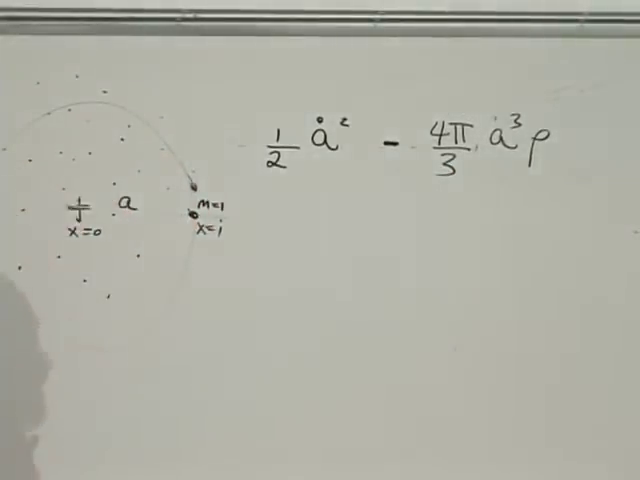
\includegraphics[width=0.78\textwidth]{lecture_03_figure_02.png}\caption{Homogene Kugel mit Mittelpunkt \(x=0\), eine komovierende Galaxie bei \(x=1\) und die Newtonsche Energiebilanz für \(a(t)\).}\end{figure}

Nur die Materie innerhalb der Kugel mit Radius \(a(t)\) trägt zur Gravitationskraft auf das Teilchen bei \(x=1\) bei. Wir setzen die Masse dieses Teilchens gleich eins. Seine kinetische Energie ist
\begin{equation}
\frac{1}{2}\dot a^2.
\end{equation}
Die innerhalb der Kugel eingeschlossene Masse beträgt
\begin{equation}
M_{\mathrm{enc}}=\frac{4\pi}{3}a^3\rho,
\end{equation}
Die gravitative potenzielle Energie ist daher
\begin{equation}
-\frac{G M_{\mathrm{enc}}}{a}
=
-\frac{4\pi G}{3}a^2\rho.
\end{equation}\editorialnote{Zum Vorlesungszeitpunkt 00:05:30 sind an der Tafel der kinetische Term und der von der Dichte abhängige Potenzialterm klar zu erkennen. Der hier notierte vollständige Koeffizient ergibt sich aus der mündlichen Herleitung.}

Aus der Energieerhaltung folgt
\begin{equation}
\frac{1}{2}\dot a^2-\frac{4\pi G}{3}a^2\rho=\text{const}.
\end{equation}
Die Konstante wird dann als \(-k\) geschrieben. Dabei gilt der übliche Vorbehalt: Die Standardnormierung legt diese Schreibweise streng genommen erst fest, nachdem die Gleichung mit \(2\) multipliziert wurde. In der Standardform lautet sie
\begin{equation}
\dot a^2=\frac{8\pi G}{3}a^2\rho-k,
\end{equation}
und Division durch \(a^2\) ergibt
\begin{equation}
\left(\frac{\dot a}{a}\right)^2=\frac{8\pi G}{3}\rho-\frac{k}{a^2}.
\end{equation}
Dies ist die Friedmann-Gleichung in der Form, die in der gesamten Diskussion verwendet wird.

\begin{figure}[ht]\centering
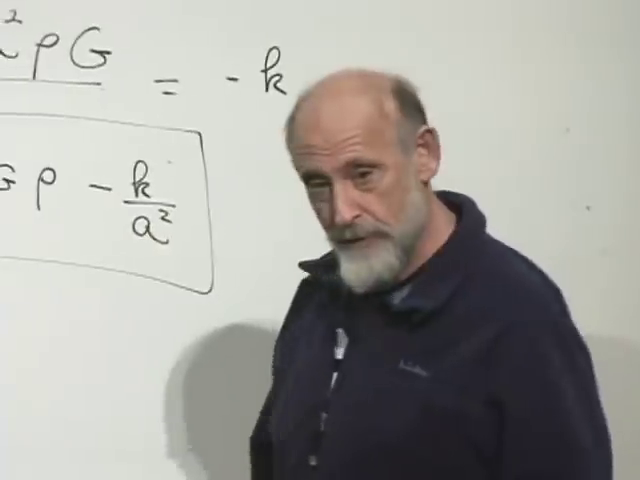
\includegraphics[width=0.56\textwidth]{lecture_03_figure_03.png}\caption{Der Krümmungsbeitrag \(-k/a^2\), isoliert in der Friedmann-Gleichung.}\end{figure}

Der Krümmungsterm ist empirisch sehr nahe bei null; so nahe, dass es auf dieser Betrachtungsebene eine sehr gute Näherung ist, ihn einfach zu vernachlässigen. Er hängt zwar mit der Krümmung des Raumes zusammen, ist hier aber beobachtungsseitig zu klein, als dass sich auch nur sein Vorzeichen bestimmen ließe.

Dieselbe Gleichung ergibt sich auch aus der allgemeinen Relativitätstheorie. Schematisch lautet die Zeit-Zeit-Komponente der Einsteinschen Gleichung
\begin{equation}
R_{00}-\frac{1}{2}g_{00}R \propto T_{00}.
\end{equation}
\editorialnote{Hier wird nur die Tensorstruktur angegeben, nicht der genaue numerische Gesamtkoeffizient.}
Bei einer expandierenden homogenen Metrik ergibt die geometrische Seite die Kombination aus \(\dot a/a\) und \(k/a^2\), während die Materieseite die Energiedichte liefert. An dieser Stelle sagen das Newtonsche Argument und die Einsteinsche Gleichung dasselbe aus.

Damit ändert sich auch die Bedeutung von \(\rho\). Von nun an ist es besser, \(\rho\) als Energiedichte zu bezeichnen. Für langsam bewegte Materie im komovierenden Bezugssystem ist das einfach die Ruheenergiedichte.

\section{Materiedominierte Epoche}

Nehmen wir nun an, dass die Energiedichte von Materie getragen wird, die im komovierenden Bezugssystem ruht. Betrachten wir einen Würfel mit einer Koordinatenlänge von einer Einheit. Seine physikalischen Seitenlängen betragen \(a(t)\), sein physikalisches Volumen also \(a^3(t)\). Wenn die Masse-Energie in diesem komovierenden Würfel \(M\) beträgt und sich die Materie mit der Strömung bewegt, statt die Begrenzung zu überqueren, gilt
\begin{equation}
\rho_m=\frac{M}{a^3}.
\end{equation}

Dies ist der materiedominierte Fall. In dieser Idealisierung ruhen die Teilchen in der Box, daher setzen wir die Temperatur und den Druck gleich null. Druck würde Teilchen erfordern, die die Begrenzung der Box überqueren.

Mit \(k\approx 0\) wird die Gleichung zu
\begin{equation}
\left(\frac{\dot a}{a}\right)^2=\frac{8\pi G}{3}\frac{M}{a^3}.
\end{equation}
Wir versuchen einen Potenzansatz:
\begin{equation}
a(t)=Ct^p.
\end{equation}
Dann gilt
\begin{equation}
\frac{\dot a}{a}=\frac{p}{t},
\end{equation}
Die linke Seite skaliert also wie \(t^{-2}\), die rechte Seite dagegen wie \(t^{-3p}\). Der Vergleich der Potenzen ergibt
\begin{equation}
3p=2,
\qquad
p=\frac{2}{3}.
\end{equation}
Folglich gilt
\begin{equation}
a(t)\propto t^{2/3}.
\end{equation}
Mit dem Koeffizienten erhält man
\begin{equation}
C^3=6\pi G M.
\end{equation}

Entscheidend an der Lösung ist das Potenzgesetz. Ein materiedominiertes Universum expandiert mit der Zweidrittelpotenz der Zeit, nicht linear. Dieses Gesetz beschreibt eine lange Zwischenphase, die ungefähr \(10^5\) Jahre nach dem Urknall beginnt und einige Milliarden Jahre später endet. Das heutige Universum ist nicht im wörtlichen Sinn materiedominiert, denn inzwischen dominiert die Dunkle Energie. Gewöhnliche Materie und ein großer Abschnitt der kosmischen Geschichte lassen sich jedoch so beschreiben.

\section{Strahlungsdominierte Epoche}

Zu noch früheren Zeiten wurde die Energiedichte von Strahlung dominiert. Der Grund ist einfach: Das Universum enthält enorm viele Photonen, ungefähr \(10^9\) Photonen auf jedes Proton. Wird das Universum komprimiert, gewinnen diese Photonen an Energie.

Ein Photon hat keine Ruhemasse, aber es besitzt Energie. Seine Energie ist
\begin{equation}
E_\gamma=h\nu=\frac{hc}{\lambda}.
\end{equation}
Entscheidend ist die Annahme, dass sich die Photonenwellenlängen bei der Expansion des Universums mit ausdehnen:
\begin{equation}
\lambda\propto a.
\end{equation}
Eine Welle in einer Box veranschaulicht das gut. Wenn die Box größer wird, wächst die Wellenlänge der Mode mit ihr. Dieselbe Vorstellung wenden wir hier auf das expandierende Universum an.

Da \(\lambda\propto a\), skaliert die Energie jedes Photons wie
\begin{equation}
E_\gamma\propto a^{-1}.
\end{equation}
Betrachten wir erneut eine komovierende Einheitsbox. Photonen treten ein und aus, aber im Mittel bleibt ihre Anzahl darin konstant. Daher skaliert auch die gesamte Photonenergie in der Box wie \(a^{-1}\). Teilt man durch das physikalische Volumen \(a^3\), so skaliert die Energiedichte der Strahlung wie
\begin{equation}
\rho_r\propto a^{-4}.
\end{equation}

Dieser zusätzliche Faktor \(a^{-1}\) macht den ganzen Unterschied aus. Materie verdünnt sich durch die Expansion des Universums. Strahlung verdünnt sich aus demselben Grund und zusätzlich dadurch, dass jedes Photon rotverschoben wird.

Die Friedmann-Gleichung für ein strahlungsdominiertes Universum lautet daher
\begin{equation}
\left(\frac{\dot a}{a}\right)^2=\frac{8\pi G}{3}\frac{M_r}{a^4}.
\end{equation}\editorialnote{In der mündlichen Diskussion wird das Symbol \(M\) für diese neue Konstante wiederverwendet. Der Index \(r\) wird hier nur hinzugefügt, um Verwechslungen mit dem Materiefall zu vermeiden.}

Wir verwenden denselben Ansatz \(a(t)=Ct^p\). Die linke Seite skaliert erneut wie \(t^{-2}\), die rechte Seite dagegen wie \(t^{-4p}\). Der Vergleich der Potenzen ergibt
\begin{equation}
4p=2,
\qquad
p=\frac{1}{2}.
\end{equation}
Also gilt
\begin{equation}
a(t)\propto t^{1/2}.
\end{equation}
Mit dem Koeffizienten erhält man
\begin{equation}
C^4=\frac{32\pi G}{3}M_r.
\end{equation}

\begin{classroomqa}\lecturetimestamp{00:35:41}\audiencequestion{Warum steht da ein \(G\)}\lecturerresponse{Weil die Energiedichte gravitativ wirkt, nicht allein die Ruhemasse. Bei langsam bewegter Materie ist der Unterschied leicht zu übersehen, aber Photonen machen ihn deutlich: Sie haben keine Ruhemasse und wirken trotzdem gravitativ.}\end{classroomqa}

Eine Box voller Strahlung veranschaulicht den Punkt. Drückt man auf eine mit Photonen gefüllte Box, so wird nach deren Beschleunigung die Wand, die sich auf die Photonen zubewegt, stärker getroffen als die Wand, die sich von ihnen entfernt. Daher muss man stärker gegen den Strahlungsdruck drücken. Die Box hat somit zusätzliche Trägheit, und nach dem Äquivalenzprinzip bedeutet diese zusätzliche Trägheit auch zusätzliche gravitative Masse. Darauf beruht hier das Argument mit der Photonenbox: Energie wirkt gravitativ.

\begin{classroomqa}\lecturetimestamp{00:38:11}\audiencequestion{Lässt sich eine dieser Gleichungen mit einem \(a\) lösen, das mit der Zeit abnimmt?}\lecturerresponse{Ja. Nimmt man den Krümmungsterm \(k/a^2\) wieder hinzu, gibt es Lösungen, bei denen das Universum zunächst expandiert und sich anschließend wieder zusammenzieht. Das scheint unserem Universum nicht zu entsprechen, aber die Gleichung lässt eine solche Entwicklung zu.}\end{classroomqa}

\begin{classroomqa}\lecturetimestamp{00:38:44}\audiencequestion{Was ist aus der Energieerhaltung geworden?}\lecturerresponse{Nimmt man den Term \(k\) wieder hinzu und multipliziert die Gleichung mit \(a^2\) zurück, ist die kosmologische Gleichung genau das Erhaltungsgesetz. Materie oder Strahlung auf der einen Seite ist nur ein Teil der Bilanz. Die Expansion trägt den kinetischen und gravitativen Anteil bei, und die Gesamtbilanz bleibt erhalten.}\end{classroomqa}

\section{Materie und Strahlung zusammen}

In der realen Kosmologie gibt es sowohl Materie als auch Strahlung. Ihre Dichten skalieren unterschiedlich:
\begin{equation}
\rho_m\propto a^{-3},
\qquad
\rho_r\propto a^{-4}.
\end{equation}
Bei kleinen \(a\) dominiert also die Strahlung. Bei großen \(a\) dominiert die Materie. Rückwärts betrachtet muss das frühe Universum daher strahlungsdominiert gewesen sein.

\begin{figure}[ht]\centering
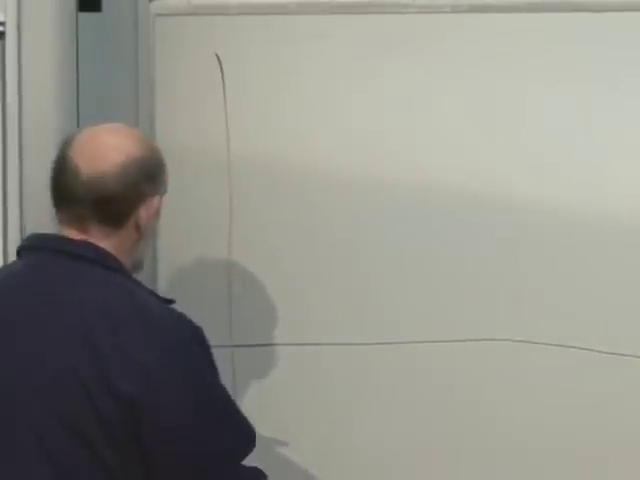
\includegraphics[width=0.68\textwidth]{lecture_03_figure_05.png}\caption{Achsen zum Vergleich der Materie- und Strahlungsenergiedichte als Funktionen des Skalenfaktors.}\end{figure}

\editorialnote{Zum Vorlesungszeitpunkt 00:44:45 sind zu Beginn der Vergleichsdiagramms an der Tafel nur die Achsen zu sehen. Die unmittelbar danach besprochenen Materie- und Strahlungskurven werden im Text beschrieben, aber hier nicht erneut eingezeichnet.}

Die Materiekurve fällt wie \(a^{-3}\). Die Strahlungskurve fällt wie \(a^{-4}\). Beide divergieren für \(a\to 0\), aber dort steigt die Strahlungskurve schneller an, sodass sich die beiden Kurven bei einem Gleichheits-Skalenfaktor schneiden. Eine grobe Schätzung datiert diesen Übergang auf ungefähr \(10^4\) Jahre, vielleicht etwas später.

Derselbe Sachverhalt lässt sich in einem Diagramm von \(a(t)\) gegen \(t\) darstellen. Früh verhält sich die Expansion wie \(t^{1/2}\), später wie \(t^{2/3}\). Der Übergang erfolgt nicht sprunghaft, sondern kontinuierlich über einen relativ engen Zeitbereich.

\begin{classroomqa}\lecturetimestamp{00:44:04}\audiencequestion{Geht die Potenz \(p\) mit dem Alter des Universums kontinuierlich von \(1/2\) zu \(2/3\) über?}\lecturerresponse{Ja. Sie springt nicht. Der Übergang ist kontinuierlich, obwohl er sich über einen ziemlich engen Zeitbereich erstreckt.}\end{classroomqa}

\section{Temperatur, Rekombination und letzte Streuung}

Als Nächstes betrachten wir die Temperatur. Wenn die Energie eines typischen Photons wie \(a^{-1}\) skaliert, dann tut dies auch die Temperatur des Strahlungsbads:
\begin{equation}
T\propto a^{-1}.
\end{equation}
Verdoppelt sich \(a\), halbiert sich die Temperatur.

Setzen wir die heutige Photonentemperatur mit etwa \(3\,\mathrm K\) und die Ionisierungstemperatur mit etwa \(3000\,\mathrm K\) an, ungefähr der Temperatur der Sonnenoberfläche. Dann gilt
\begin{equation}
\frac{a_{\mathrm{today}}}{a_{\mathrm{ion}}}\sim 10^3.
\end{equation}
Mit dem Gesetz \(a\propto t^{2/3}\) für die materiedominierte späte Epoche ergibt sich
\begin{equation}
\left(\frac{t_{\mathrm{today}}}{t_{\mathrm{ion}}}\right)^{2/3}\sim 10^3,
\end{equation}
also
\begin{equation}
\frac{t_{\mathrm{today}}}{t_{\mathrm{ion}}}\sim 1000^{3/2}\sim 3\times 10^4.
\end{equation}
Setzen wir für diese Abschätzung das Alter des Universums mit \(10^{10}\) Jahren an, erhalten wir
\begin{equation}
t_{\mathrm{ion}}\sim 3\times 10^5\ \mathrm{years}.
\end{equation}

Dies ist die Epoche, in der Wasserstoff und Helium aufhören, vollständig ionisiert zu sein. Davor ist das Universum ein heißes Plasma. Warum ist ein Plasma undurchsichtig? Weil freie Ladungen stark auf elektromagnetische Wellen reagieren. Das elektrische Feld treibt die Ladungen hin und her; das Medium verhält sich wie ein Leiter, und Leiter sind undurchsichtig. Darin liegt die einschlägige Analogie zur Sonnenoberfläche.

Sobald das Universum so weit abgekühlt ist, dass Elektronen mit Atomkernen rekombinieren, entstehen gewöhnliche neutrale Atome und das Universum wird deutlich transparenter. Der Übergang ist nicht unendlich scharf. Es handelt sich um einen unscharfen Ort oder ein unscharfes Zeitintervall, aber für die Kosmologie ist er scharf genug, um als Oberfläche der letzten Streuung bezeichnet zu werden.

Wer nach außen blickt, blickt in der Zeit zurück. Nahe Galaxien zeigen die jüngere Vergangenheit. Weiter entfernte Galaxien zeigen frühere Zeiten. Weit genug entfernt trifft jede Sichtlinie auf die Epoche, in der das Universum noch ionisiert und undurchsichtig war. Elektromagnetische Strahlung kann nichts zeigen, was davor liegt.

Andere Boten könnten prinzipiell noch frühere Zeiten sondieren. Neutrinos sind elektrisch neutral und würden früher entkoppeln. Gravitonen würden, falls sie sich je beobachten ließen, aus noch früheren Epochen stammen. Doch dieselbe schwache Wechselwirkung, die es ihnen ermöglichen würde, das frühe Plasma zu durchdringen, macht sie auch extrem schwer nachweisbar.

Wenn das Universum einst in alle Richtungen so heiß wie die Sonnenoberfläche war, warum blendet uns der Himmel dann nicht? Weil sich die Oberfläche der letzten Streuung von uns entfernt und die von dort eintreffenden Photonen ungefähr um denselben Faktor \(10^3\) rotverschoben wurden, der \(3000\,\mathrm K\) von \(3\,\mathrm K\) unterscheidet. Bei uns kommt Mikrowellenstrahlung an, kein sichtbares Sonnenlicht.

\begin{classroomqa}\lecturetimestamp{01:03:51}\audiencequestion{Können unsere Teleskope also nicht weiter zurückblicken als bis ungefähr \(300{,}000\) Jahre?}\lecturerresponse{Mit elektromagnetischen Teleskopen nicht. Davor war das Universum ionisiert und undurchsichtig. Andere Boten könnten zumindest prinzipiell frühere Epochen sondieren.}\end{classroomqa}

\begin{classroomqa}\lecturetimestamp{01:08:43}\audiencequestion{Wenn Sie von der Temperatur eines Photons sprechen, meinen Sie die Temperatur eines schwarzen Körpers mit diesem Strahlungsmaximum. Aber die hängt doch nicht linear von der Wellenlänge ab, oder?}\lecturerresponse{Richtig. Die Temperatur entspricht im Wesentlichen der Energie eines typischen Photons; für ein Photon skaliert sie daher umgekehrt proportional zur Wellenlänge. Das Gesetz \(T^4\) bezieht sich auf die Energiedichte, nicht auf die Energie eines einzelnen Photons. Es berücksichtigt sowohl die Energie pro Photon als auch die Anzahl der Photonen pro Volumeneinheit; die Teilchendichte skaliert wie \(T^3\).}\end{classroomqa}

Somit gilt
\begin{equation}
n_\gamma\propto T^3,
\qquad
\rho_\gamma\propto T^4.
\end{equation}

\section{Dunkle Materie aus Rotationskurven}

Dunkle Materie kommt über galaktische Rotationskurven ins Spiel. Sie wurde nicht aus der großräumigen Friedmann-Gleichung abgeleitet, sondern aus astronomischen Beobachtungen auf galaktischen Skalen.

Beginnen wir mit dem einfachsten Newtonschen Problem: Ein leichter Körper der Masse \(m\) umläuft eine zentrale Masse \(M\) im Abstand \(r\). Die Gravitationskraft beträgt
\begin{equation}
\frac{GMm}{r^2},
\end{equation}
und die Zentripetalbeschleunigung ist \(v^2/r\). Nach dem Newtonschen Gesetz gilt
\begin{equation}
m\frac{v^2}{r}=\frac{GMm}{r^2}.
\end{equation}
Kürzen wir \(m\) und multiplizieren mit \(r\), erhalten wir
\begin{equation}
v(r)=\sqrt{\frac{GM}{r}}.
\end{equation}
Wenn sich die gravitative Masse also nahe dem Zentrum konzentriert, nimmt die Umlaufgeschwindigkeit wie \(r^{-1/2}\) ab.

Das wäre zu erwarten, wenn die Masse der Lichtverteilung folgte. Der größte Teil der sichtbaren Materie einer Galaxie liegt nahe ihrem Kern, sodass sich äußere Sterne dann ähnlich wie Planeten in den äußeren Bereichen des Sonnensystems verhalten würden. Astronominnen und Astronomen bestimmen die Umlaufgeschwindigkeiten, indem sie die Dopplerverschiebungen auf gegenüberliegenden Seiten einer nahen Galaxie messen und dabei die sich auf uns zubewegende Seite mit der sich von uns wegbewegenden vergleichen, nachdem sie die gemeinsame Rezessionsbewegung der ganzen Galaxie herausgerechnet haben. Die gemessenen Umlaufgeschwindigkeiten bleiben bis zu großen Radien ungefähr konstant.

Ersetzen wir also die zentrale Masse \(M\) durch die eingeschlossene Masse \(M(r)\):
\begin{equation}
\frac{v^2}{r}=\frac{G M(r)}{r^2}.
\end{equation}
Ist \(v(r)\) annähernd konstant, dann gilt
\begin{equation}
M(r)\propto r.
\end{equation}
Mit anderen Worten: Die gravitative Masse nimmt mit dem Radius weiter zu, selbst dort, wo das sichtbare Licht es nicht tut.

Nehmen wir nun, der Einfachheit halber wie in der Diskussion, an, dass die Massenverteilung ungefähr kugelsymmetrisch ist. Dann gilt
\begin{equation}
M(R)=\int_0^R 4\pi r^2\rho(r)\,dr.
\end{equation}
Wenn \(M(R)\propto R\), ergibt die Ableitung nach \(R\)
\begin{equation}
4\pi R^2\rho(R)\propto 1,
\end{equation}
und somit
\begin{equation}
\rho(r)\propto \frac{1}{r^2}.
\end{equation}

\begin{classroomqa}\lecturetimestamp{01:28:18}\audiencequestion{Es sieht so aus, als müsste die Dichte wie \(1/r^2\) abnehmen. Gibt es dafür einen Grund?}\lecturerresponse{Aus der beobachteten flachen Rotationskurve folgt \(M(R)\propto R\); durch Ableiten erhält man dann \(\rho(r)\propto 1/r^2\). Darüber hinaus wird hier keine einfache Erklärung aus ersten Prinzipien beansprucht; detaillierte Simulationen leisten einen großen Teil der Arbeit.}\end{classroomqa}

Die belastbare Schlussfolgerung lautet, dass eine Galaxie wesentlich mehr gravitative Masse enthält, als allein die leuchtende Materie vermuten ließe: mehrere Male mehr, in der hier verwendeten Schätzung ungefähr eine Größenordnung mehr. Die sichtbare Galaxie liegt in einem viel größeren dunklen Halo.

Was hindert gewöhnliches Gas daran, in einem solchen diffusen Zustand zu verbleiben? Dissipation. Eine Gaswolke zieht sich zusammen, weil Stöße, reibungsähnliche Prozesse und Strahlung ihr Energie entziehen können. Dunkle Materie strahlt offenbar kaum und ist nahezu kollisionsfrei. Die Gravitation kann sie nach innen ziehen und potenzielle Energie in kinetische Energie umwandeln, doch ohne effiziente Dissipation kollabiert sie nicht zu den kompakten leuchtenden Strukturen, die gewöhnliche Materie bildet. Die kinetische Energie hält den Halo ausgedehnt.

Anschließend werden einige Alternativen mit Vorsicht erörtert. Neutrinos seien zu schnell, um sich auf galaktischen Skalen auf diese Weise zu verhalten. Ein Halo aus gewöhnlichem Wasserstoff würde die Nukleosynthese im frühen Universum erheblich stören. Auch Schwarze Löcher aus gewöhnlicher Materie werden als problematisch erwähnt, denn sie würden zu viel gewöhnliche Materie im frühen Universum voraussetzen und Fragen zur Gravitationslinsenwirkung aufwerfen. Mehr wird an dieser Stelle nicht behauptet.

Der Halo wird weder als dünne Schale noch als Torus beschrieben. Er ist eine ungefähr kugelförmige, inhomogene Materieverteilung: dichter zum Zentrum hin und nach außen allmählich abfallend.

\begin{classroomqa}\lecturetimestamp{01:53:12}\audiencequestion{Meinen Sie den Bullet-Cluster?}\lecturerresponse{Ja. Das Röntgengas zeigt die gewöhnliche Materie, während Gravitationslinsen die gesamte gravitative Masse sichtbar machen. Bei der Kollision trennen sich diese beiden Verteilungen voneinander. Das ist ein starker Beleg für reale Dunkle Materie und gegen eine bloße Modifikation der Gravitation, die allein an die sichtbare Materie gebunden ist.}\end{classroomqa}

Das ist der abschließende Beobachtungsbefund. Über die genaue Beschaffenheit der Dunklen Materie ist nur sehr wenig bekannt, doch nichts von dem hier Gesagten erfordert ein radikal neues Prinzip. Die konservative Möglichkeit ist schlicht, dass es in der Natur zusätzliche schwach wechselwirkende Teilchen gibt, die bislang nicht identifiziert wurden.

\chapter{Horizonte, Zustandsgleichung und Vakuumenergie}

\section{Bevorzugtes Bezugssystem, überlichtschnelle Entfernung und Horizont}

Der kosmische Mikrowellenhintergrund zeichnet tatsächlich ein spezielles Bezugssystem aus. In dem Bezugssystem, in dem diese Strahlung isotrop erscheint, sind im Mittel auch die nahen Galaxien in Ruhe. Bewegen wir uns durch den Hintergrund, werden Photonen in Bewegungsrichtung zu höheren Energien und Photonen in Gegenrichtung zu niedrigeren Energien Doppler-verschoben. Das bevorzugte Bezugssystem ist dasjenige, in dem der Mikrowellenhintergrund isotrop erscheint; zugleich ist es im Mittel das Bezugssystem, in dem die lokalen Galaxien in Ruhe sind.

\begin{classroomqa}\lecturetimestamp{00:00:25}\audiencequestion{Hängt die scheinbare Wellenlänge der kosmischen Strahlung von der Bewegung des Beobachters ab, und bedeutet das, dass es ein bevorzugtes Bezugssystem gibt?}\lecturerresponse{Ja. Die Bewegung durch den Mikrowellenhintergrund erzeugt eine Doppler-Anisotropie. Daher gibt es ein bevorzugtes kosmologisches Bezugssystem: dasjenige, in dem der Mikrowellenhintergrund isotrop erscheint. Zugleich ist es im Mittel das Bezugssystem, in dem die lokalen Galaxien in Ruhe sind.}\end{classroomqa}

Eine zweite Frage betrifft die Fluchtgeschwindigkeiten. Nach dem Hubble-Gesetz entfernen sich hinreichend weit entfernte Galaxien voneinander gemäß
\begin{equation}
v = H d .
\end{equation}
Für hinreichend große \(d\) übersteigt diese Fluchtgeschwindigkeit die Lichtgeschwindigkeit. Das widerspricht der Relativitätstheorie nicht, denn das Verbot gilt lokal: Kein Objekt kann unmittelbar vor uns schneller als das Licht an einem anderen vorbeiziehen. Die Aussage über weit entfernte Galaxien betrifft die Geometrie zwischen weit voneinander entfernten Orten.

\begin{classroomqa}\lecturetimestamp{00:04:48}\audiencequestion{Können zwei Galaxien eine Relativgeschwindigkeit haben, die größer ist als \(c\)?}\lecturerresponse{Ja, wenn sie weit genug voneinander entfernt sind. Die Hubble-Flucht kann die Lichtgeschwindigkeit überschreiten, ohne der lokalen Relativitätstheorie zu widersprechen. Der Ort, an dem die Fluchtgeschwindigkeit \(c\) erreicht, ist ein Horizont.}\end{classroomqa}

Sobald die Fluchtgeschwindigkeit die Lichtgeschwindigkeit erreicht, machen Signale, die auf uns zu gesendet werden, keinen Nettfortschritt mehr. Der Lichtstrahl bewegt sich lokal weiterhin mit der Grenzgeschwindigkeit, aber die zu überwindende Entfernung wächst zu schnell.

\begin{classroomqa}\lecturetimestamp{00:07:03}\audiencequestion{Würde ein Lichtstrahl, der in die entgegengesetzte Richtung ausgesandt wird, sich nicht trotzdem auf uns zubewegen?}\lecturerresponse{Lokal tut er das, aber der Raum wächst schneller, als der Strahl die Entfernung überwinden kann. Der Strahl bewegt sich relativ zu benachbarten Punkten mit der Grenzgeschwindigkeit, während die Gesamtentfernung zu uns weiter zunimmt.}\end{classroomqa}

\section{Die expandierende Metrik und die Analogie mit einer Linie}

Ein anschauliches Bild ergibt sich in einer Dimension. Stellen wir uns eine Linie aus Atomen vor. Dehnen wir eine gewöhnliche materielle Linie, reißt sie irgendwann. Ändern wir nun das Bild: Immer wenn sich benachbarte Atome zu weit voneinander entfernen, fügen wir ein weiteres Atom dazwischen ein. Die Linie wächst weiter, aber ihre lokalen Eigenschaften dünnen nicht aus.

\begin{figure}\centering
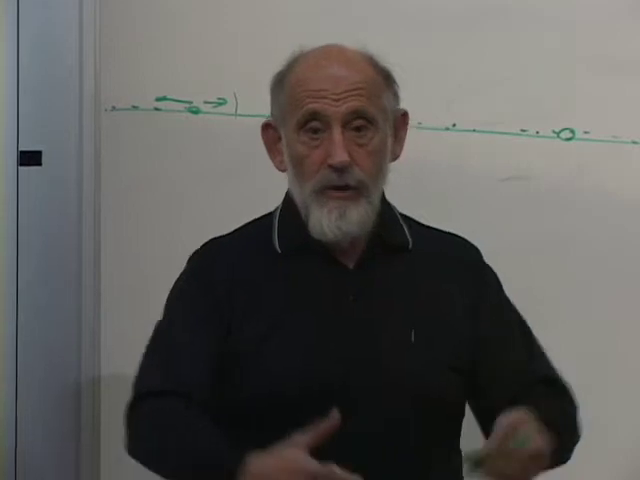
\includegraphics[width=0.60\textwidth]{lecture_04_figure_02.png}\caption{Eindimensionale Linie zur Veranschaulichung einer expandierenden Metrik.}\end{figure}

In diesem Bild gibt es weiterhin eine lokale Grenzgeschwindigkeit für Signale, so wie Schall auf einer gewöhnlichen Linie eine Grenzgeschwindigkeit hat. Die Regel gilt lokal: Eine Störung kann sich relativ zu benachbarten Punkten nicht schneller ausbreiten. Ist die Linie jedoch lang genug und werden schnell genug neue Punkte eingefügt, entfernen sich weit genug voneinander entfernte Teile so rasch, dass ein Signal niemals zurückgelangen kann.

Die relativistische Geschwindigkeitsaddition ist daher nur ein Teil der Geschichte. Sie gilt lokal, wenn Beobachter am selben Ort aneinander vorbeiziehen. Für weit voneinander entfernte Galaxien in einer expandierenden Geometrie ist sie nicht das geeignete Werkzeug.

\begin{classroomqa}\lecturetimestamp{00:09:42}\audiencequestion{Gilt in dieser Situation weiterhin das gewöhnliche relativistische Gesetz für die Addition von Geschwindigkeiten?}\lecturerresponse{Lokal, an einem Ort, ja. Ziehen Beobachter nacheinander aneinander vorbei, gilt die gewöhnliche spezielle relativistische Regel. Sie eignet sich jedoch nicht zur Beschreibung der Flucht weit voneinander entfernter Galaxien mit mehr als \(c\); dafür muss man auf die Geometrie des expandierenden Raums zurückgreifen.}\end{classroomqa}

Dasselbe Bild liefert eine einfache Erklärung der Rotverschiebung. Zeichnet man eine Welle auf die Linie, wächst ihre Wellenlänge mit der Linie mit, wenn diese expandiert. In einer expandierenden Geometrie ist das nicht bloß ein anschauliches Bild. Wellengleichungen in der expandierenden Raumzeit ergeben tatsächlich gestreckte Wellenlängen.

\begin{classroomqa}\lecturetimestamp{00:14:42}\audiencequestion{Ist die Aussage, dass sich eine Welle mit dem Universum ausdehnt, theoretisch, empirisch oder beides?}\lecturerresponse{Sie folgt theoretisch aus der Wellenausbreitung in der expandierenden Raumzeit und wird außerdem durch astronomische Beobachtungen gestützt.}\end{classroomqa}

Dieses Bild ist kein Gummiband. Ein Gummiband wird beim Dehnen dünner, und jemand, der in einem solchen Medium lebt, würde Veränderungen der lokalen Eigenschaften feststellen. Hier bleiben die lokalen Eigenschaften gleich, während der globale Maßstab der Entfernungen wächst.

\section{Letzte Streuung und das beobachtbare Universum}

Der Horizont ist der Ort, an dem die Fluchtgeschwindigkeit die Lichtgeschwindigkeit erreicht. Die Oberfläche der letzten Streuung liegt knapp innerhalb davon. Ein Signal, das vom Horizont ausgesandt würde, wäre unbeschränkt rotverschoben; die Strahlung der letzten Streuung weist eine enorme, aber endliche Rotverschiebung auf.

\begin{classroomqa}\lecturetimestamp{00:17:53}\audiencequestion{Wie hängen überlichtschnelle Flucht, die Oberfläche der letzten Streuung und das beobachtbare Universum zusammen?}\lecturerresponse{Der Horizont ist der Ort, an dem die Fluchtgeschwindigkeit die Lichtgeschwindigkeit erreicht. Die Oberfläche der letzten Streuung liegt knapp innerhalb davon, da ihre Rotverschiebung enorm, aber endlich ist. Praktisch gesehen markiert sie den Rand des beobachtbaren Universums.}\end{classroomqa}

Die Rotverschiebung der Strahlung von der letzten Streuung beträgt ungefähr den Faktor \(10^3\). Dieser Wert ist bereits so groß, dass die Oberfläche der letzten Streuung für viele Zwecke sehr nahe am Horizont liegt. Das beobachtbare Universum ist der Teil des Universums, aus dem Licht uns erreichen kann.

Zu späten Zeiten nähert sich die Expansion dem vakuumdominierten Regime. Dann strebt die Hubble-Größe einem konstanten Wert zu, der Horizont nähert sich einer festen Größe, und sowohl Galaxien als auch Mikrowellenstrahlung verschwinden nach und nach aus unserem Blickfeld.

\begin{classroomqa}\lecturetimestamp{00:22:43}\audiencequestion{Da sich \(H\) mit der Zeit ändert, ändert sich dann auch die Horizontentfernung, und wird der Mikrowellenhintergrund irgendwann verschwinden?}\lecturerresponse{Zu späten Zeiten strebt \(H\) einem konstanten Wert zu, sodass sich der Horizont einer festen Entfernung nähert. Der Mikrowellenhintergrund wird weiterhin gedehnt, kühlt ab und verblasst. Auch weit entfernte Galaxien überschreiten den Horizont und verschwinden aus unserem Blickfeld.}\end{classroomqa}

Sichtbar bleiben nur Strukturen, die bereits gravitativ gebunden sind. Das Sonnensystem fliegt nicht auseinander, und auch die Galaxie fliegt nicht auseinander, doch das Universum wird im großen Maßstab zu einer isolierten Insel.

\section{Die grundlegende Expansionsgleichung und die drei Komponenten}

Die grundlegende Expansionsgleichung lautet nun
\begin{equation}
\left(\frac{\dot a}{a}\right)^2 = \frac{8\pi G}{3}\rho ,
\qquad c=1 .
\end{equation}
Dabei ist \(a(t)\) der Skalenfaktor und \(\rho\) die Gesamtenergiedichte.

\begin{figure}\centering
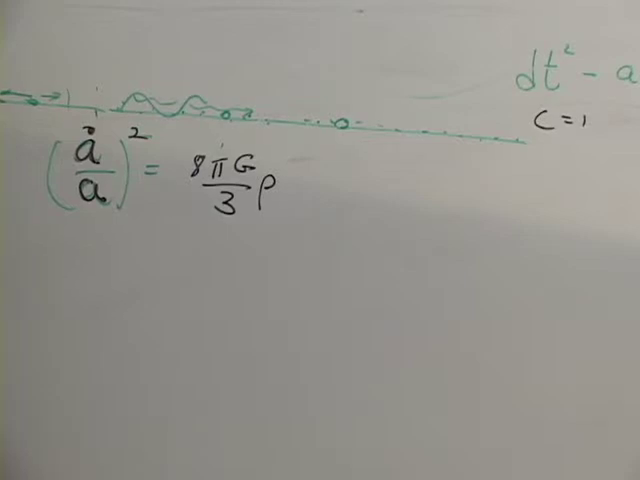
\includegraphics[width=0.74\textwidth]{lecture_04_figure_03.png}\caption{Grundlegende Expansionsgleichung und Analogie mit der eindimensionalen Linie.}\end{figure}

Drei Komponenten sind dynamisch bedeutsam.

Für Materie gilt
\begin{equation}
\rho=\frac{\text{const.}}{a^3},
\qquad
a(t)\sim t^{2/3}.
\end{equation}
Das ist der Fall massiver Objekte, die sich mit der Gesamtexpansion bewegen und im mitbewegten Bezugssystem im Wesentlichen in Ruhe sind.

Für Strahlung gilt
\begin{equation}
\rho=\frac{\text{const.}}{a^4},
\qquad
a(t)\sim t^{1/2}.
\end{equation}
Die zusätzliche Potenz von \(a\) ergibt sich daraus, dass jedes Photon bei der Expansion des Universums rotverschoben wird.

Außerdem gibt es
\begin{equation}
\rho_0=\text{constant},
\end{equation}
die Vakuumenergie, auch dunkle Energie genannt oder, bis auf übliche numerische Faktoren, die kosmologische Konstante. Diese Komponente verdünnt sich überhaupt nicht.

Als Nächstes muss die Energiedichte mit dem Druck in Beziehung gesetzt werden.

\section{Strahlungsdruck und kalte Materie}

Beginnen wir mit Strahlung. Betrachten wir einen eindimensionalen Kasten, also einfach ein Liniensegment der Länge \(L\), in dem Photonen hin und her reflektiert werden. In einer Dimension sind Kraft und Druck praktisch dasselbe.

Betrachten wir ein Photon mit dem Impulsbetrag \(p\). Bei der Reflexion an einer Wand ändert sich sein Impuls um
\begin{equation}
\Delta p = 2p.
\end{equation}
Die Zeit zwischen zwei aufeinanderfolgenden Stößen an derselben Wand beträgt
\begin{equation}
\Delta t = \frac{2L}{c}.
\end{equation}
Die mittlere Kraft auf die Wand ist daher
\begin{equation}
F=\frac{\Delta p}{\Delta t}=\frac{pc}{L}.
\end{equation}
Für ein Photon gilt
\begin{equation}
E=pc,
\end{equation}
also
\begin{equation}
F=\frac{E}{L}.
\end{equation}
Die Energie geteilt durch die Länge ist die eindimensionale Energiedichte. In diesem eindimensionalen Fall gilt
\begin{equation}
P=\rho .
\end{equation}

Bei vielen Photonen bleibt derselbe Zusammenhang nach der Mittelung erhalten. Die Gesamtkraft entspricht einfach der Gesamtenergie pro Längeneinheit.

Gehen wir nun zu drei Dimensionen über. Bewegten sich alle Photonen nur entlang einer Achse, würden sie Druck auf ein Paar von Flächen ausüben und auf die übrigen Flächen keinen. Das ist bewusst falsch angesetzt, zeigt aber unmittelbar, was korrigiert werden muss. In einem isotropen Strahlungsbad ist der Impuls auf alle Richtungen verteilt. Im Mittel trägt ein Drittel der Energiedichte zu jeder Druckkomponente bei. Das Ergebnis lautet
\begin{equation}
P=\frac{\rho}{3}.
\end{equation}

Für kalte Materie fällt das Ergebnis anders aus. Betrachten wir einen mitbewegten Kasten, also ein kleines Gebiet, das sich mit der Strömung des Universums bewegt. Die Teilchen darin tragen Energie, aber wenn sie relativ zum Kasten in Ruhe sind, stoßen sie nicht gegen seine Wände. Der Druck ist daher
\begin{equation}
P=0.
\end{equation}

\begin{figure}\centering
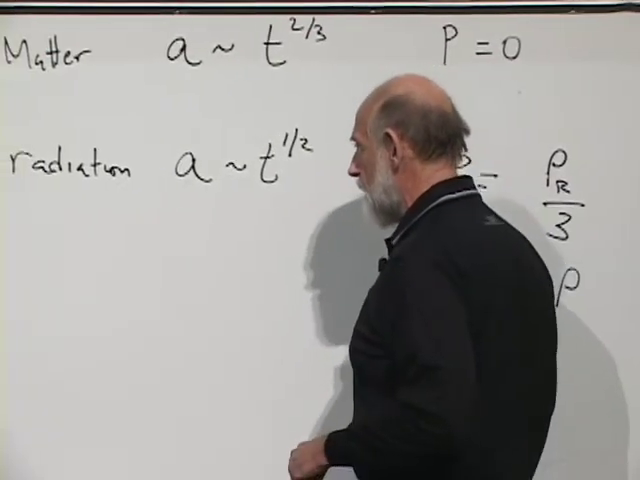
\includegraphics[width=0.74\textwidth]{lecture_04_figure_04.png}\caption{Materie und Strahlung: \(a\sim t^{2/3}\), \(P=0\) und \(a\sim t^{1/2}\), \(P=\rho/3\).}\end{figure}

Die Zusammenfassung an der Tafel lautet
\begin{align}
\text{matter:}\qquad & a(t)\sim t^{2/3}, \qquad P=0,\\
\text{radiation:}\qquad & a(t)\sim t^{1/2}, \qquad P=\frac{\rho}{3}.
\end{align}

\begin{classroomqa}\lecturetimestamp{00:54:27}\audiencequestion{Bewegen sich die Teilchen im expandierenden Universum nicht tatsächlich voneinander weg?}\lecturerresponse{Ja, aber die Druckbetrachtung bezieht sich auf einen infinitesimal kleinen mitbewegten Kasten. Auf dieser lokalen Skala gilt die thermodynamische Argumentation weiterhin.}\end{classroomqa}

\section{Die Zustandsgleichung}

Der Druck wird als proportional zur Energiedichte angenommen:
\begin{equation}
P=w\rho .
\end{equation}
An der Tafel wird derselbe Parameter mit \(\omega\) bezeichnet. Für die beiden grundlegenden Fälle gilt
\begin{equation}
w=0 \quad \text{for cold matter},
\qquad
w=\frac{1}{3} \quad \text{for radiation}.
\end{equation}

Auch Zwischenfälle sind möglich. Werte zwischen \(0\) und \(1/3\) beschreiben Materie, die weder vollständig kalt noch voll relativistisch ist. Als Beispiel wird hier warme dunkle Materie genannt.

\begin{figure}\centering
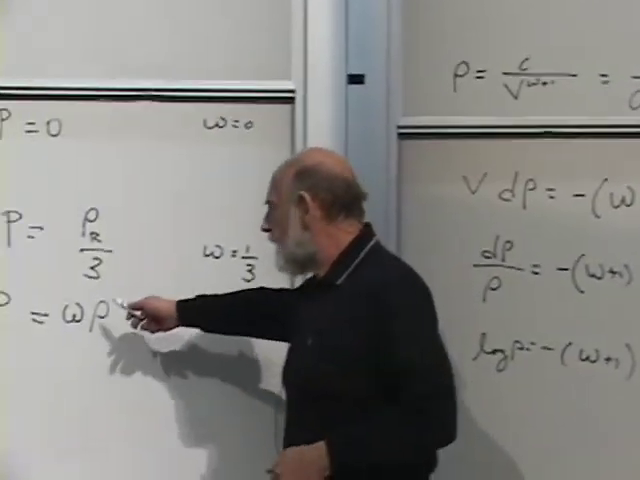
\includegraphics[width=0.74\textwidth]{lecture_04_figure_05.png}\caption{Zustandsgleichung \(P=\omega\rho\) zusammen mit der Herleitung der Skalierung der Dichte.}\end{figure}

Als Nächstes stellt sich die Frage, ob \(w\) die Abhängigkeit von \(\rho\) von \(a\) bestimmt. Die Antwort ergibt sich aus einer thermodynamischen Identität.

Betrachten wir einen Kasten mit Volumen \(V\). Übt der Inhalt einen Druck \(P\) aus, so verrichtet er bei einer Volumenzunahme des Kastens um \(dV\) an den Wänden die Arbeit
\begin{equation}
dE=-P\,dV.
\end{equation}
Schreiben wir nun die Energie als
\begin{equation}
E=\rho V.
\end{equation}
Ihr Differential lautet
\begin{equation}
dE=\rho\,dV+V\,d\rho .
\end{equation}
Setzt man die beiden Ausdrücke gleich, erhält man
\begin{equation}
\rho\,dV+V\,d\rho=-P\,dV,
\end{equation}
oder
\begin{equation}
V\,d\rho=-(\rho+P)\,dV.
\end{equation}
Mit \(P=w\rho\) folgt
\begin{equation}
V\,d\rho=-(1+w)\rho\,dV.
\end{equation}
Teilen wir durch \(\rho V\):
\begin{equation}
\frac{d\rho}{\rho}=-(1+w)\frac{dV}{V}.
\end{equation}
Durch Integration ergibt sich
\begin{equation}
\rho \propto V^{-(1+w)}.
\end{equation}
Für einen kosmologischen, mitbewegten Kasten gilt
\begin{equation}
V\propto a^3,
\end{equation}
und damit
\begin{equation}
\rho \propto a^{-3(1+w)}.
\end{equation}

Damit erhält man unmittelbar die zuvor betrachteten Fälle zurück:
\begin{align}
w=0 &\Longrightarrow \rho \propto a^{-3},\\
w=\frac{1}{3} &\Longrightarrow \rho \propto a^{-4}.
\end{align}

Deshalb ist \(w\) von Bedeutung. Sobald \(\rho(a)\) bekannt ist, kann man es wieder in die Friedmann-Gleichung einsetzen. Dann nimmt man ein Potenzgesetz \(a\sim t^\alpha\) an und bestimmt, wie sich das Universum für diese Zustandsgleichung ausdehnt.

\section{Vakuumenergie und negativer Druck}

Ein besonderer Fall verhält sich anders:
\begin{equation}
w=-1.
\end{equation}
Dann gilt
\begin{equation}
1+w=0,
\end{equation}
Der Exponent verschwindet also, und es gilt
\begin{equation}
\rho=\rho_0=\text{constant}.
\end{equation}
Der zugehörige Druck ist
\begin{equation}
P=-\rho .
\end{equation}

Negativer Druck ist an sich nicht rätselhaft. Positiver Druck drückt die Wände eines Kastens nach außen. Negativer Druck zieht sie nach innen. Er entspricht einer Spannung. Ein gedehntes Gummiband ist ein alltägliches Beispiel: Es speichert positive Energie, zieht seine Enden aber zusammen.

Setzen wir die konstante Dichte \(\rho_0\) in die Friedmann-Gleichung ein:
\begin{equation}
\left(\frac{\dot a}{a}\right)^2=\frac{8\pi G}{3}\rho_0.
\end{equation}
Die rechte Seite ist einfach eine Zahl, also gilt
\begin{equation}
\frac{\dot a}{a}=\sqrt{\frac{8\pi G}{3}\rho_0}.
\end{equation}
In diesem besonderen Fall ist die Hubble-Größe tatsächlich konstant. Die Gleichung lässt sich schreiben als
\begin{equation}
\dot a=\sqrt{\frac{8\pi G}{3}\rho_0}\,a,
\end{equation}
und die Lösung lautet
\begin{equation}
a(t)\propto \exp\!\left(\sqrt{\frac{8\pi G}{3}\rho_0}\,t\right).
\end{equation}

Das ist exponentielle Expansion. Die maßgebliche Zeitskala ist die \(e\)-fache Zeit, nicht die Verdopplungszeit; die hier verwendete grobe Abschätzung ordnet sie in die Größenordnung des Alters des Universums ein. Vakuumenergie und kosmologische Konstante bezeichnen denselben physikalischen Bestandteil, abgesehen von historischen Konventionen für numerische Faktoren.

\begin{classroomqa}\lecturetimestamp{01:27:16}\audiencequestion{Wenn Vakuumenergie exponentielle Expansion antreibt, wird dann nicht irgendwann alles auseinandergerissen?}\lecturerresponse{Nicht unbedingt. Gebundene Systeme können ihr widerstehen. Eine Galaxie, ein Sonnensystem oder ein Atom muss nicht auseinandergerissen werden, während hinreichend große und dünn verteilte Strukturen an der Expansion teilhaben und sich schließlich voneinander entfernen.}\end{classroomqa}

\begin{classroomqa}\lecturetimestamp{01:31:43}\audiencequestion{Hat das negative Vorzeichen beim Ziehen der Quadratwurzel aus der Friedmann-Gleichung eine interessante Bedeutung?}\lecturerresponse{Ja. Die Quadratwurzel liefert zwei Zweige. Einer ist die expandierende Lösung, der andere die zeitumgekehrte kontrahierende Lösung. Die Gleichungen selbst lassen beide zu.}\end{classroomqa}

\section{Drei Epochen und die beobachtete Expansionsgeschichte}

Alle drei Komponenten sind vorhanden und skalieren unterschiedlich:
\begin{equation}
\begin{aligned}
\rho_{\text{radiation}}&\propto a^{-4},\\
\rho_{\text{matter}}&\propto a^{-3},\\
\rho_0&=\text{constant}.
\end{aligned}
\end{equation}
Daraus folgen unmittelbar drei Epochen.

Bei sehr kleinem \(a\) dominiert die Strahlung. Später dominiert Materie. Bei hinreichend großem \(a\) dominiert die Vakuumenergie. Die zugehörigen Expansionsgesetze lauten
\begin{equation}
a(t)\sim t^{1/2},
\qquad
a(t)\sim t^{2/3},
\qquad
a(t)\sim e^{Ht}.
\end{equation}

Die hier genannten ungefähren Zeitpunkte sind folgende: Nach etwa \(10^4\) Jahren geht die Strahlungsdominanz in die Materiedominanz über. Später, nach etwa \(10^5\) Jahren, wird das Universum durchsichtig. Der Übergang von der Materiedominanz zur beschleunigten Expansion erfolgt viel später, nach mehreren Milliarden Jahren, in der hier verwendeten Größenordnungsschätzung ungefähr zur Halbzeit der kosmischen Geschichte.

Wie lässt sich diese Geschichte erschließen? Die Zukunft können wir nicht sehen, wohl aber die Vergangenheit. Größere Entfernung bedeutet, dass wir weiter in die Vergangenheit blicken. Indem man weit entfernte Galaxien beobachtet, misst, wie ihre Bewegung mit ihrer Entfernung zusammenhängt, und die Hubble-Größe als Funktion der Rückblickzeit rekonstruiert, lässt sich der zeitliche Verlauf des Skalenfaktors bestimmen. Die strahlungsdominierte Epoche liegt zu früh, um sie direkt mit gewöhnlicher Galaxienastronomie zu beobachten. Die materiedominierte Epoche und der Übergang zur Vakuumdominanz sind jedoch in der rekonstruierten Kurve sichtbar.

\section{Letzte Streuung in ferner Zukunft}

Der Mikrowellenhimmel in ferner Zukunft erzählt eine andere Geschichte als Galaxien, die den Horizont überschreiten. Die Strahlung, die wir zu späteren Zeiten sehen, stammt von weiter entfernter Materie. Der Effekt besteht also darin, weiter und kühler in die Tiefe des Universums zu blicken, und nicht darin, dass dieselben Atome einfach immer weiter davonfliegen.

\begin{classroomqa}\lecturetimestamp{01:48:07}\audiencequestion{Wenn die Oberfläche der letzten Streuung im Horizont verblasst, ist das dasselbe wie Galaxien, die sich über den Horizont hinausbewegen?}\lecturerresponse{Nein. Die spätere Strahlung stammt nicht von denselben Atomen wie die Strahlung, die wir jetzt sehen. Sie stammt von Atomen, die weiter entfernt waren. Es ist, als blickte man immer tiefer in das Universum, während die Strahlung immer kühler erscheint.}\end{classroomqa}

\section{Krümmung, das Bild des Big Crunch und der Horizont zu späten Zeiten}

Bislang wurde der Krümmungsterm weggelassen. Nimmt man ihn wieder hinzu, ergibt sich
\begin{equation}
\left(\frac{\dot a}{a}\right)^2
=
\frac{8\pi G}{3}\rho
-
\frac{K}{a^2}.
\end{equation}
Numerisch scheint dieser Term klein zu sein, begrifflich ist er jedoch wichtig. In der älteren Newtonschen Sprache unterscheidet er Fälle positiver, verschwindender und negativer Gesamtenergie. In der relativistischen Sprache unterscheidet er die räumlichen Geometrien.

Bevor Vakuumenergie ernst genommen wurde, stellte man sich häufig ein materiedominiertes Universum vor, in dem sich die Expansion schließlich umkehren würde. Daraus ergab sich das alte Bild des Big Crunch: Expansion nach dem Urknall, gefolgt von einer erneuten Kontraktion. Die Mathematik gilt weiterhin, scheint aber unser Universum nicht mehr zu beschreiben.

\begin{classroomqa}\lecturetimestamp{01:53:51}\audiencequestion{Hängt diese Vakuumenergie mit der quantenmechanischen Vakuumenergie zusammen?}\lecturerresponse{Ja, oder zumindest glaubt man das.}\end{classroomqa}

Die ungefähre Zusammensetzung heute ist
\begin{equation}
\frac{\rho_0}{\rho_{\text{total}}}\sim 0.7,
\qquad
\frac{\rho_{\text{matter}}}{\rho_{\text{total}}}\sim 0.3.
\end{equation}
Von der Materiekomponente entfallen etwa \(0.05\) der Gesamtmenge auf leuchtende Materie und etwa \(0.25\) auf dunkle Materie. Strahlung ist heute vernachlässigbar. Dunkle und leuchtende Materie skalieren gleich, daher bleibt ihr Verhältnis konstant, auch wenn sich die relativen Anteile von Materie, Strahlung und Vakuum von Epoche zu Epoche ändern.

Im vakuumdominierten Grenzfall gilt
\begin{equation}
H=\sqrt{\frac{8\pi G}{3}\rho_0}.
\end{equation}
Dann wird das Hubble-Gesetz zu
\begin{equation}
v=Hd.
\end{equation}
Der Horizont ist durch \(v=1\) definiert, seine Entfernung beträgt also
\begin{equation}
d_H=\frac{1}{H}
=
\frac{1}{\sqrt{8\pi G\rho_0/3}}.
\end{equation}
Die hier genannte grobe Größenordnung liegt bei \(10\) bis \(12\) Milliarden Lichtjahren.

Entscheidend ist das Verhalten zu späten Zeiten. Sobald die Expansion exponentiell verläuft, wird die Horizontentfernung konstant. Galaxien überschreiten ihn weiterhin und verschwinden, indem sie immer stärker rotverschoben werden. Auch der Mikrowellenhintergrund wird immer weiter rotverschoben. In ferner Zukunft bleiben nur die nahen gravitativ gebundenen Strukturen sichtbar, und das Universum erscheint wie eine isolierte Insel.

\section{Geometrie anhand der Oberfläche der letzten Streuung}

Schließlich lässt sich die Geometrie anhand der Oberfläche der letzten Streuung prüfen. Nehmen wir an, die Entfernung zu dieser Oberfläche sei bekannt. Nehmen wir außerdem an, man könne dort eine Verdichtung ausmachen, deren physikalische Größe hinreichend genau bekannt ist. Dann kann man diese Größe und Entfernung mit der beobachteten Winkelausdehnung vergleichen.

In einem flachen Raum entspricht der Winkel dem euklidischen Wert. In einem positiv gekrümmten Raum erschiene das Objekt größer, in einem negativ gekrümmten kleiner. Die Analogie ist eine gewöhnliche Vermessung: Man nimmt ein Objekt bekannter Größe in bekannter Entfernung und vergleicht den gemessenen Winkel mit dem Wert, den die euklidische Geometrie vorhersagt.

\begin{classroomqa}\lecturetimestamp{02:08:09}\audiencequestion{Was ist ein Beispiel für ein Objekt dort draußen, dessen Größe wir kennen?}\lecturerresponse{Die größten Verdichtungen im Mikrowellenhintergrund. Wir glauben, ihre Größe aus der Zeit, die sie für ihre Entwicklung benötigten, und aus der Schallgeschwindigkeit zu kennen.}\end{classroomqa}

Hier geht es um die größten Verdichtungen im Mikrowellenhintergrund. Ihre beobachtete Winkelausdehnung stimmt bis auf wenige Prozent mit der euklidischen Geometrie überein. Auf dieser Grundlage erscheint der Raum flach.

\section{Gemessenes \(w\) und eine abschließende Frage}

Die Beobachtungsbedeutung von \(w\) ist nun klar. Wenn Astronomen berichten, dass \(w\) sehr nahe bei \(-1\) liegt, sagen sie damit, dass die Vakuumenergiekomponente nahezu konstant ist. Genau das ist der hier dargelegte Punkt.

Das bedeutet nicht, dass die allgemeine Relativitätstheorie \(w\) zwingend genau auf \(-1\) festlegt. Hier geht es um eine empirische Aussage. In der Vorlesung wird kurz erwähnt, dass grundsätzlich auch radikalere Möglichkeiten nicht ausgeschlossen sind. Für den Fall einer nahezu konstanten Vakuumenergie gibt es jedoch gute Gründe, ihn für plausibel zu halten.

\begin{classroomqa}\lecturetimestamp{02:11:04}\audiencequestion{Haben wir bei der Berechnung der Dichte für Materie und Strahlung angenommen, dass die Energie konstant ist, und dann den Skalenfaktor angepasst, um die Formel zu bestimmen? Und falls das für die ersten beiden Fälle gilt: Was geschieht dann im Fall der Vakuumenergie, bei der die Dichte konstant bleibt?}\lecturerresponse{Nein. Ich habe nicht angenommen, dass sie konstant ist. Wir haben verwendet, dass sich die Energie um \(-P\,dV\) ändert. Bei einem gedachten mitbewegten Kasten, der sich zusammen mit der Expansion bewegt, wird an den Wänden Arbeit verrichtet; das erklärt die Energieänderung. Der Fall der Vakuumenergie wirft die Frage auf andere Weise auf. Zum Abschluss sei dazu gesagt, dass die Rede von Energieerhaltung in der Kosmologie nicht viel aussagt, weil die Gesamtenergie des Universums null ist.}\end{classroomqa}
\chapter{Kugeln, hyperbolischer Raum und die Bedeutung von \(k\)}

Betrachten wir ein wenig Mathematik, einfache Mathematik. Kugeln in beliebig vielen Dimensionen sind besondere Geometrien: Sie sind homogen, und homogen bedeutet hier konstante Krümmung. Zuerst betrachten wir positive Krümmung, dann homogene negative Krümmung und anschließend den Zusammenhang mit den Einsteinschen Feldgleichungen.

Ein kugelförmiges Universum bedeutet, dass \emph{der Raum} kugelförmig ist, nicht die Raumzeit. Es gibt auch die andere Möglichkeit: homogene negative Krümmung. Stellt man diese Fälle einander gegenüber, wird die Rolle der allgemeinen Relativitätstheorie deutlich.

\section{Kugeln und homogene Geometrie}

Eine eindimensionale Kugel ist einfach ein Kreis. Am einfachsten beschreibt man ihn, indem man ihn in einen zweidimensionalen Hilfsraum einbettet und schreibt:
\begin{equation}
x^2+y^2=R^2.
\end{equation}
Die eindimensionale Einheitskugel ist gegeben durch
\begin{equation}
x^2+y^2=1.
\end{equation}

Eine zweidimensionale Kugel wird genauso beschrieben, nun mit drei Hilfskoordinaten:
\begin{equation}
x^2+y^2+z^2=R^2,
\end{equation}
Im Einheitsfall gilt
\begin{equation}
x^2+y^2+z^2=1.
\end{equation}

Diese Koordinaten sind lediglich eine Krücke. Die Geometrie, um die es geht, ist nicht der umgebende \(x,y,z\)-Raum. Sie ist die Oberfläche selbst. Ein Lebewesen, das auf einer eindimensionalen Kugel lebt, lebt auf einem Kreis; es hat keinen Zugang zu einem Inneren oder einem Äußeren. Dasselbe gilt für eine zweidimensionale Kugel. Das Kugelinnere und der Außenraum gehören nur zum Hilfsbild.

Mit derselben Konstruktion erhält man eine dreidimensionale Kugel. Man führt eine weitere Koordinate ein, etwa \(w\), und schreibt:
\begin{equation}
x^2+y^2+z^2+w^2=R^2,
\end{equation}
Im Einheitsfall gilt
\begin{equation}
x^2+y^2+z^2+w^2=1.
\end{equation}
Eine dreidimensionale Kugel lässt sich schwerer veranschaulichen, denn die Krücke wäre nun vierdimensional. Die Mathematik ist jedoch kaum schwieriger.

Die übliche Schreibweise für die \(n\)-dimensionale Kugel ist \(\Omega_n\). Somit ist \(\Omega_1\) die eindimensionale, \(\Omega_2\) die zweidimensionale und \(\Omega_3\) die dreidimensionale Kugel.

\section{Metriken auf der Kugel}

Nützlicher ist eine intrinsische Beschreibung. Dabei beschreibt man die Kugel durch Koordinaten, die auf der Kugel selbst liegen.

Für die eindimensionale Einheitskugel genügt eine Koordinate \(\phi\) mit \(0\leq \phi \leq 2\pi\). Ihre Metrik lautet
\begin{equation}
ds^2=d\phi^2.
\end{equation}
Man schreibt auch
\begin{equation}
d\Omega_1^2=d\phi^2.
\end{equation}

Die zweidimensionale Einheitskugel lässt sich als Folge eindimensionaler Kugeln beschreiben. Ein Winkel \(\phi\) läuft weiterhin einmal um jeden Kreis, während ein zweiter Winkel \(\theta\) von einem Ende der Kugel zum anderen verläuft. Dieser zweite Winkel reicht von \(0\) bis \(\pi\). Eine Bewegung in \(\theta\)-Richtung trägt den Term \(d\theta^2\) bei. Die Bewegung in \(\phi\)-Richtung erfolgt auf einem Kreis mit dem Radius \(\sin\theta\). Somit gilt
\begin{equation}
d\Omega_2^2=d\theta^2+\sin^2\theta\,d\phi^2
\end{equation}
oder
\begin{equation}
d\Omega_2^2=d\theta^2+\sin^2\theta\,d\Omega_1^2.
\end{equation}

Die dreidimensionale Kugel erhält man auf dieselbe Weise, nun als Folge zweidimensionaler Kugeln. Dazu führt man eine weitere Koordinate \(\alpha\) ein. Dann gilt
\begin{equation}
d\Omega_3^2=d\alpha^2+\sin^2\alpha\,d\Omega_2^2.
\end{equation}
Ausmultipliziert ergibt sich
\begin{equation}
d\Omega_3^2=d\alpha^2+\sin^2\alpha\left(d\theta^2+\sin^2\theta\,d\phi^2\right).
\end{equation}
Hier läuft \(\alpha\) von einem Ende mit verschwindender Größe zum anderen, also gilt \(0\leq \alpha \leq \pi\).\editorialnote{Bei 00:17:24 klingt es in der Audioaufnahme kurz wie „``null bis zwei Pi''“. Die umgebende Konstruktion und der ausdrückliche Faktor \(\sin^2\alpha\) erfordern jedoch, dass die neue Koordinate von einem Ende der Familie niedrigerdimensionaler Kugeln mit verschwindender Größe zum anderen läuft.}

Die allgemeine rekursive Form lautet
\begin{equation}
d\Omega_n^2=d\alpha^2+\sin^2\alpha\,d\Omega_{n-1}^2.
\end{equation}

Hat man diese Sichtweise übernommen, kann man das Einbettungsbild vergessen. Eine eindimensionale Kugel wird durch eine Koordinate beschrieben, eine zweidimensionale durch zwei, eine dreidimensionale durch drei und so weiter. Die Geometrie besteht für sich.

Diese Geometrie ist besonders, weil sie homogen ist. Man könnte die Metrik verformen, indem man \(\sin^2\theta\) durch eine andere Funktion ersetzte, die an beiden Enden weiterhin verschwindet. So erhielte man eine verformte geschlossene Fläche, etwa ein Ellipsoid. Sie wäre dann aber nicht mehr homogen. Die Kugel ist homogen, weil jeder Punkt jedem anderen gleicht.

Soll eine Kugel den Radius \(A\) statt Einheitsradius haben, multipliziert man die Einheitsmetrik mit \(A^2\):
\begin{equation}
ds^2=A^2\,d\Omega_3^2.
\end{equation}
Das Quadrat ist erforderlich, weil die Metrik das Abstandsquadrat misst.

Ein kurzer Einschub betrifft die nulldimensionale Kugel. Geht man einen Schritt zurück, erhält man
\begin{equation}
x^2=1,
\end{equation}
mit den beiden Lösungen \(x=\pm 1\). Die nulldimensionale Einheitskugel besteht also einfach aus zwei Punkten.

\section{Ein kugelförmiges FRW-Universum}

Nun geht es nicht mehr nur um den Raum, sondern um die Raumzeit. Das relevante Bild ist eine dreidimensionale Kugel, deren Radius sich mit der Zeit ändert.

Dabei ist durchgehend eine Warnung zu beachten: Die Zeit ist etwas anderes. Man sollte sich das expandierende Universum nicht als höherdimensionale Kugel vorstellen, bei der die Zeit die Rolle einer weiteren Einbettungskoordinate spielt.

Mit diesem Vorbehalt lautet das Raumzeitintervall
\begin{equation}
d\tau^2=dt^2-a(t)^2\,d\Omega_3^2.
\end{equation}
Dies ist die FRW-Metrik für ein räumlich kugelförmiges Universum. Gegenüber der statischen Kugel besteht die einzige Neuerung darin, dass der Radius nun eine zeitabhängige Funktion \(a(t)\) ist.

Praktisch ist es, die Koordinaten so zu wählen, dass wir uns an einem Pol befinden. Dieser Punkt ist nicht besonders; die Wahl ist lediglich eine Konvention. Dann lässt sich \(\alpha\) als radiale Koordinate auf der Einheitskugel, ausgehend von uns, auffassen. Es ist keine radiale Entfernung in Kilometern. Es ist ein dimensionsloses Winkelmaß auf der Einheitskugel, das in der Geometrie jedoch die Rolle einer radialen Entfernung spielt.

Abgesehen von lokalen Ansammlungen wie Galaxien und Sternen ist dies die gesamte Geometrie eines räumlich kugelförmigen FRW-Universums. Seine räumliche Krümmung ist positiv; die Vorzeichenkonvention lautet
\begin{equation}
k=+1.
\end{equation}
Das bedeutet nicht, dass irgendetwas selbst „``plus eins''“ ist. Es bedeutet lediglich, dass die räumliche Krümmung positiv ist.

\section{Blick von einer Kugel nach außen}

Wie sieht eine solche Kugel aus, wenn man von einem ihrer Punkte nach außen blickt? Hier kommt die stereografische Projektion ins Spiel.

Man betrachte eine zweidimensionale Kugel, die eine unendliche Ebene am Südpol berührt. Wählt man einen Punkt auf der Kugel, zieht man eine Gerade vom Nordpol durch diesen Punkt und verlängert sie, bis sie die Ebene trifft. So wird jedem Punkt auf der Kugel ein Punkt in der Ebene zugeordnet. Der Südpol wird auf den Ursprung der Ebene abgebildet. Der Nordpol ist der Ausnahmefall: Nähert man sich ihm aus verschiedenen Richtungen, wandert sein Bild richtungsabhängig ins Unendliche. Daher behandelt man ihn als den Punkt im Unendlichen.

Platziert man gleich große ``Kontinente'' an verschiedenen Stellen auf der Kugel, werden ihre Bilder auf der Ebene größer, je näher man dem Nordpol kommt. Ein Beobachter am Südpol würde also weit entfernte Objekte unter größeren Winkeln sehen als im flachen Raum. Bei positiver Krümmung erscheint ein Objekt bekannter Größe im Vergleich zur euklidischen Geometrie zu groß.

Das ist der grundlegende Beobachtungspunkt. Auf Krümmung schließt man aus dem Zusammenhang zwischen Entfernung, Größe und Winkelausdehnung. Galaxien eignen sich für sehr große Entfernungen nicht als gute Standardmaßstäbe, aber die Logik ist genau diese.

\begin{classroomqa}
\lecturetimestamp{00:45:54}
\audiencequestion{Muss man neben der Winkelausdehnung auch die Entfernung kennen?}
\lecturerresponse{Ja. Der Winkel allein reicht nicht aus. Man braucht den Winkel und die Entfernung.}
\end{classroomqa}

\begin{classroomqa}
\lecturetimestamp{00:46:18}
\audiencequestion{Werden Kreise auf der Kugeloberfläche als Kreise projiziert?}
\lecturerresponse{Ja. Kreise werden als Kreise projiziert. Das ist eine der besonderen Eigenschaften der stereografischen Projektion.}
\end{classroomqa}

\begin{classroomqa}
\lecturetimestamp{00:47:02}
\audiencequestion{Behält ein Kontinent bei der Projektion seine Form?}
\lecturerresponse{Hier sind zwei verschiedene Aussagen zu unterscheiden. Die eine besagt, dass Kreise als Kreise projiziert werden. Die andere, schwächere Aussage besagt, dass hinreichend kleine Formen ihre lokale Form behalten, weil die Winkel erhalten bleiben. Die Abbildung ist konform: Sie erhält die Winkel, aber nicht die relativen Größen.}
\end{classroomqa}

\section{Homogene negative Krümmung}

Der Fall homogener negativer Krümmung wird über seine Metrik eingeführt.

Das Analogon zur Kugel bei negativer Krümmung ist der hyperbolische Raum. Im selben rekursiven Sinn wie zuvor erhält man seine Metrik, indem man \(\sin\alpha\) durch \(\sinh\alpha\) ersetzt:
\begin{equation}
d\mathcal H_n^2=d\alpha^2+\sinh^2\alpha\,d\Omega_{n-1}^2.
\end{equation}
Der niedrigerdimensionale Winkelanteil bleibt die Metrik der Einheitskugel \(d\Omega_{n-1}^2\).

\begin{classroomqa}
\lecturetimestamp{00:55:51}
\audiencequestion{Ist das niedrigerdimensionale Differential in der Metrik weiterhin das der Kugel?}
\lecturerresponse{Ja. Dieser niedrigerdimensionale Anteil ist die gewöhnliche Metrik der Einheitskugel. Geändert hat sich der davorstehende Faktor \(\sinh^2\alpha\).}
\end{classroomqa}

Der hyperbolische Sinus ist
\begin{equation}
\sinh\alpha=\frac{e^\alpha-e^{-\alpha}}{2}.
\end{equation}
Das Minuszeichen ist wichtig; in der Vorlesung wird es sogleich von einem Studenten korrigiert.

Ein entscheidender Unterschied besteht auch im Wertebereich der Koordinate. Bei der Kugel läuft die neue Koordinate von einem Ende zum anderen und endet bei \(\pi\). Hier gilt
\begin{equation}
0\leq \alpha<\infty.
\end{equation}
Der gewöhnliche Sinus steigt zunächst an und fällt dann wieder auf null. Der hyperbolische Sinus beginnt bei \(\alpha=0\) auf dieselbe Weise, wächst dann aber exponentiell.

Das bedeutet, dass die niedrigerdimensionalen Kugeln um uns herum immer größer werden, je weiter wir uns nach außen bewegen. In dieser Geometrie wächst der Himmel mit zunehmendem Radius zunächst nicht und schrumpft dann wieder. Er wächst immer weiter.

In drei räumlichen Dimensionen lautet die entsprechende FRW-Form
\begin{equation}
d\tau^2=dt^2-a(t)^2\,d\mathcal H_3^2,
\end{equation}
und die Vorzeichenangabe lautet
\begin{equation}
k=-1.
\end{equation}

\section{Das Bild der Kreisscheibe und seine Bedeutung}

Negative Krümmung wird im durch Escher berühmt gewordenen Bild der Kreisscheibe anschaulich, besonders in \emph{Grenzkreis IV}. Die Analogie zur stereografischen Projektion ist hilfreich, aber das Verhalten ist umgekehrt.

Bei der Kugel sieht die Projektion unendlich aus, obwohl die tatsächliche Geometrie endlich ist. Bei negativer Krümmung sieht das Bild der Kreisscheibe endlich aus, obwohl die tatsächliche Geometrie unendlich ist. Gleich große ``Kontinente'' oder ``Galaxien'' erscheinen immer kleiner, je näher man sich dem Rand nähert; geometrisch sind sie jedoch alle gleich groß. Misst man die Entfernung, indem man zählt, wie viele gleich große Abschnitte man durchquert, liegt der Rand unendlich weit entfernt.

Ein Objekt bekannter Größe erscheint bei negativer Krümmung also im Vergleich zum flachen Raum zu klein. Es nimmt einen zu kleinen Winkel ein.

Die Geometrie ist weiterhin homogen. Auch wenn im Bild die äußeren Abschnitte winzig erscheinen, würde jeder Beobachter an einem anderen Ort dieselbe intrinsische Geometrie sehen.

\begin{classroomqa}
\lecturetimestamp{01:06:42}
\audiencequestion{Würde ein Beobachter in einem beliebigen dieser Kreise ein ähnliches Muster sehen?}
\lecturerresponse{Ja, genau dasselbe. Der Raum ist homogen.}
\end{classroomqa}

\begin{classroomqa}
\lecturetimestamp{01:07:03}
\audiencequestion{Im kugelförmigen Fall erscheinen weit entfernte Dinge also zu groß, hier dagegen zu klein?}
\lecturerresponse{Ja. Bei positiver Krümmung nimmt ein Objekt bekannter Größe im Vergleich zum flachen Raum einen zu großen Winkel ein. Bei negativer Krümmung nimmt es einen zu kleinen Winkel ein.}
\end{classroomqa}

\begin{classroomqa}
\lecturetimestamp{01:08:09}
\audiencequestion{Besteht die Bedeutung der Projektion nach Art der stereografischen Projektion darin, dass ein Astronom sie aus Beobachtungen rekonstruieren kann?}
\lecturerresponse{Ja. Der Astronom ist im Grunde ein Vermesser, der Dreiecke am Himmel vermisst. Um den unmittelbaren geometrischen Punkt zu betrachten, kann man von der Zeitabhängigkeit absehen und sich auf Winkel und Entfernungen konzentrieren.}
\end{classroomqa}

Es gibt auch ein nützliches Bild für den lokalen Bereich. Eine kleine Fläche negativer Krümmung lässt sich als Sattelfläche im gewöhnlichen dreidimensionalen Raum zeichnen. Auf kleine Flächen ist das jedoch beschränkt; die gesamte hyperbolische Ebene lässt sich nicht global als eine schöne gewöhnliche Fläche im dreidimensionalen euklidischen Raum einbetten.

\section{Der flache Fall}

Zwischen den Fällen positiver und negativer Krümmung liegt der flache Raum. Man kann ihn als Grenzfall betrachten; es genügt aber, ihn einfach als gewöhnlichen flachen euklidischen Raum aufzufassen.

Seine FRW-Form lautet
\begin{equation}
d\tau^2=dt^2-a(t)^2\left(dx^2+dy^2+dz^2\right),
\end{equation}
mit
\begin{equation}
k=0.
\end{equation}

Dies sind die drei homogenen FRW-Geometrien:
\begin{align}
k=+1 &: \text{positive spatial curvature},\\
k=0 &: \text{flat space},\\
k=-1 &: \text{negative spatial curvature}.
\end{align}

\begin{classroomqa}
\lecturetimestamp{01:15:07}
\audiencequestion{Wenn man die Geometrie auf eine Ebene projiziert und einem Signal folgt, würde sich dann die projizierte Lichtgeschwindigkeit von Ort zu Ort ändern?}
\lecturerresponse{Ja, in der Projektion würde sie sich ändern. In der Kugelprojektion schiene das Licht weiter außen immer schneller zu werden; auf der Scheibe mit negativer Krümmung schiene es sich am Rand immer langsamer zu bewegen. Diese Änderung gehört zum Bild, nicht zur zugrunde liegenden Physik.}
\end{classroomqa}

\begin{classroomqa}
\lecturetimestamp{01:17:05}
\audiencequestion{Hat man tatsächlich schon einmal weit entfernte Objekte auf diese Weise betrachtet, um festzustellen, ob der Raum flach ist?}
\lecturerresponse{Ja, aber dabei nutzt man tatsächlich die Winkelinformation. Man bestimmt die Flachheit nicht, indem man zu messen versucht, wie schnell sich Licht in der Projektion zu bewegen scheint.}
\end{classroomqa}

\section{Zurück zu den kosmologischen Gleichungen}

Nach der Pause folgt der Zusammenhang zwischen den bereits behandelten kosmologischen Gleichungen und den Einsteinschen Feldgleichungen. Zu diesem Zeitpunkt ist an der Tafel noch der Ausschnitt der flachen räumlichen Metrik zu sehen.

\begin{figure}[htbp]
\centering
\includegraphics[width=0.72\textwidth]{lecture_05_figure_02.png}
\caption{Ausschnitt der flachen FRW-Metrik.}
\lectureframe{01:18:18}
\end{figure}

Zunächst eine sehr kurze Wiederholung der Newtonschen Betrachtung. Wir befinden uns im Zentrum und betrachten eine Galaxie, die sich gemäß dem Hubble-Gesetz von uns entfernt. Nach dem Newtonschen Theorem für eine kugelsymmetrische Verteilung trägt nur die Masse innerhalb der Kugel, deren Radius der Entfernung der Galaxie entspricht, zur auf sie wirkenden Kraft bei. Dann gibt es drei Möglichkeiten: Die Galaxie bewegt sich mit mehr als der Fluchtgeschwindigkeit, mit weniger als der Fluchtgeschwindigkeit oder genau mit der Fluchtgeschwindigkeit.

Als Nächstes sei in Erinnerung gerufen: Bei gewöhnlicher nichtrelativistischer Materie ist die Dichte proportional zur Masse dividiert durch \(a^3\), bei Strahlung ist sie proportional zu \(1/a^4\), und bei Vakuumenergie ändert sie sich nicht, wenn sich die Kugel verändert.

In der früheren Newtonschen Behandlung enthielt die kosmologische Gleichung einen Dichteterm und, sofern man nicht genau den Fall der Fluchtgeschwindigkeit betrachtete, zusätzlich einen konstanten Term proportional zu \(1/a^2\). In der früheren Diskussion wurde dieser Term meist gleich null gesetzt. Empirisch ist er klein, aber begrifflich gibt es keinen Grund, ihn wegzulassen.

\section{Die Einsteinschen Feldgleichungen und die \(00\)-Komponente}

Als Nächstes kommen die Einsteinschen Feldgleichungen. Auf der linken Seite steht die Geometrie, die durch die Raumzeitkrümmung bestimmt ist. Auf der rechten Seite steht der Energie-Impuls-Tensor, die Quelle des Gravitationsfelds. In der Normierung der Vorlesung schreibt man
\begin{equation}
R^{\mu\nu}-\frac{1}{2}g^{\mu\nu}R=4\pi G\,T^{\mu\nu}.
\end{equation}
\editorialnote{Der Faktor \(\tfrac12\) ist in der sichtbaren Zeile an der Tafel nicht lesbar, wird aber bei 01:33:36 in der gesprochenen Korrektur wieder eingesetzt. Die Gleichung hier enthält diese Korrektur und behält zugleich die Normierung \(4\pi G\) der Vorlesung bei.}

Hier werden nicht alle zehn unabhängigen Komponenten benötigt. Inzwischen wurde bereits so viel vorausgesetzt --- Homogenität, die FRW-Form und ein einziger zeitabhängiger Skalenfaktor ---, dass nur noch eine freie Funktion übrig ist, nämlich \(a(t)\). Naheliegend ist die Wahl der Zeit-Zeit-Komponente, denn \(T^{00}\) ist die Energiedichte \(\rho\).

\begin{figure}[htbp]
\centering
\includegraphics[width=0.62\textwidth]{lecture_05_figure_05.png}
\caption{Einsteinsche Feldgleichung und ihre \(00\)-Komponente.}
\lectureframe{01:30:54}
\end{figure}

Wir konzentrieren uns also auf
\begin{equation}
R^{00}-\frac{1}{2}g^{00}R=4\pi G\,\rho.
\end{equation}

Die rechte Seite ist die Energiedichte. Die linke Seite ist die Geometrie.

\begin{classroomqa}
\lecturetimestamp{01:39:09}
\audiencequestion{Was ist mit den anderen Komponenten des Energie-Impuls-Tensors?}
\lecturerresponse{Sie verschwinden im Allgemeinen nicht. Die Raum-Raum-Komponenten können den Druck darstellen. Im materiedominierten Fall ist der Druck null, im strahlungsdominierten Fall beträgt er ein Drittel der Energiedichte, und für Vakuumenergie schreibt man \(P=w\rho\) mit \(w=-1\).}
\end{classroomqa}

\begin{classroomqa}
\lecturetimestamp{01:40:24}
\audiencequestion{Würden also bei ausschließlichem Vorhandensein von Materie die anderen Komponenten von \(T^{\mu\nu}\) verschwinden?}
\lecturerresponse{Bei druckloser Materie verschwinden die Druckkomponenten, ja.}
\end{classroomqa}

\section{Was die Einsteinsche Rechnung ergibt}

Die vollständige Krümmungsrechnung wird an der Tafel nicht durchgeführt. Entscheidend ist, was sich ergibt, wenn man eine FRW-Metrik in den Einsteintensor einsetzt.

Ein Term entsteht allein dadurch, dass der Skalenfaktor von der Zeit abhängt. Selbst wenn der Raum flach wäre, würde ein zeitabhängiger Skalenfaktor weiterhin Raumzeitkrümmung erzeugen. Dieser Beitrag ist proportional zu
\begin{equation}
\left(\frac{\dot a}{a}\right)^2.
\end{equation}

Der zweite Term entsteht durch die räumliche Krümmung selbst. Selbst wenn der Skalenfaktor zeitlich konstant wäre, würde der gekrümmte Raum zur Raumzeitkrümmung beitragen. Bei einer einfachen Geometrie mit konstanter Krümmung ist die Krümmung proportional zum Kehrwert des Krümmungsradius zum Quadrat. Daher trägt sie einen Term proportional zu
\begin{equation}
\frac{k}{a^2},
\end{equation}
bei: mit positivem Vorzeichen für die Kugel, negativem Vorzeichen für den hyperbolischen Fall und null für den flachen Raum.

\begin{classroomqa}
\lecturetimestamp{01:36:53}
\audiencequestion{Müsste es nicht auch einen Faktor wie etwa einen Krümmungsradius geben?}
\lecturerresponse{Dieser steckt bereits im Faktor \(1/a^2\). Bei diesen einfachen Geometrien mit konstanter Krümmung ist die Krümmung einfach der Kehrwert des Krümmungsradius zum Quadrat.}
\end{classroomqa}

Die Koeffizienten werden während der Rechnung mitgeführt und teilweise anhand des früheren Newtonschen Ergebnisses überprüft. Am Ende erhält man\footnote{Diese angegebene Friedmann-Form fasst die mündliche, selbst korrigierte Diskussion der Koeffizienten und den Vergleich mit dem früheren Newtonschen Ergebnis bei 01:32:35--01:36:53 zusammen.}
\begin{equation}
\left(\frac{\dot a}{a}\right)^2+\frac{k}{a^2}=\frac{8\pi G}{3}\rho,
\end{equation}
oder äquivalent
\begin{equation}
\left(\frac{\dot a}{a}\right)^2=\frac{8\pi G}{3}\rho-\frac{k}{a^2}.
\end{equation}

Diese Form verknüpft die drei FRW-Geometrien mit der zuvor behandelten kosmologischen Dynamik.

\begin{classroomqa}
\lecturetimestamp{01:37:52}
\audiencequestion{Könnte \(k\) durch eine Neudefinition von \(a\) jeden beliebigen Wert annehmen?}
\lecturerresponse{Im flachen Fall gibt es für \(a\) keine ausgezeichnete natürliche Skala, daher kann man es skalieren; \(k\) bleibt dabei jedoch null. In den Fällen positiver und negativer Krümmung gibt es eine natürliche Krümmungsskala. Setzt man \(a(t)\) gleich diesem natürlichen Krümmungsradius, so ist \(k\) einfach \(+1\) oder \(-1\).}
\end{classroomqa}

\begin{classroomqa}
\lecturetimestamp{01:41:00}
\audiencequestion{Ist \(k\) in der endgültigen Gleichung gleich \(+1\), \(-1\) oder \(0\)?}
\lecturerresponse{Ja. Für die Kugel ist es \(+1\), für den hyperbolischen Fall \(-1\) und für den flachen Raum \(0\).}
\end{classroomqa}

Die Newtonsche Behandlung hat uns nicht in die Irre geführt; sie ergab dieselbe grundlegende Gleichung. Was die allgemeine Relativitätstheorie hinzufügt, ist die Interpretation. Aus Newtonscher Sicht unterscheidet die zusätzliche Konstante, ob die Geschwindigkeit über oder unter der Fluchtgeschwindigkeit liegt oder genau dem Grenzfall entspricht. Aus Einsteinscher Sicht gibt dasselbe Vorzeichen die Geometrie des Raums selbst an.

\begin{classroomqa}
\lecturetimestamp{01:42:46}
\audiencequestion{Wie funktionierte das, bevor man eine kosmologische Konstante einführte?}
\lecturerresponse{Vor Einführung der kosmologischen Konstante bestand ein enger Zusammenhang zwischen dem Verhalten bezüglich der Fluchtgeschwindigkeit und der räumlichen Geometrie. Für \(k=+1\) ist der Raum positiv gekrümmt und die Bewegung liegt unter der Fluchtgeschwindigkeit, sodass das Universum expandieren und anschließend wieder kontrahieren kann. Für \(k=-1\) ist der Raum negativ gekrümmt und die Bewegung liegt über der Fluchtgeschwindigkeit, sodass das Universum immer weiter expandiert. Für \(k=0\) liegt der marginale Grenzfall vor.}
\end{classroomqa}

Dasselbe Vorzeichen \(k\) lässt sich daher auf zwei Arten deuten: als dynamische Klassifikation der Bewegung und als Vorzeichen der räumlichen Krümmung.
\chapter{Letzte Streuung und Baryogenese}

\section{Weiter hinauszuschauen heißt, in die Vergangenheit zu blicken}

In verschiedenen Entfernungen sehen wir das Universum zu verschiedenen Zeiten. In unserer Nähe ist die Rückblickzeit nicht besonders wichtig. Das Universum vor einem Jahr oder vor hundert Jahren unterschied sich kaum vom heutigen. Doch weit genug entfernt sehen wir das Universum in einem jüngeren Zustand. Ein jüngeres Universum ist dichter, und ein dichteres Universum ist heißer.

In einer hinreichend großen Entfernung war das Universum ungefähr so heiß wie die Sonnenoberfläche. Für uns sieht es nicht so aus, weil die Photonen auf ihrem Weg hierher rotverschoben wurden. Ein Rotverschiebungsfaktor von etwa tausend bedeutet, dass die beobachtete Temperatur um denselben Faktor niedriger ist:
\[
T_{\mathrm{obs}} \sim \frac{T_{\mathrm{emit}}}{1+z},
\qquad
1+z \sim 10^3.
\]\footnote{Diese Darstellung ist eine kompakte redaktionelle Transkription des mündlichen Arguments zur Rotverschiebung bei 00:02:20--00:02:39.}

Dort wurde das Universum undurchsichtig. Es bestand hauptsächlich aus Wasserstoff und zu einem kleinen Teil aus Helium. Bei Temperaturen von mehreren tausend Grad ist Wasserstoff ionisiert. Jenseits dieser Oberfläche gibt es also keine neutralen Atome, sondern Ionen: vor allem Protonen und Elektronen, die sich frei bewegen. Auch die Photonen sind dort energiereicher, im Wesentlichen Röntgenstrahlung. Falls sich zufällig ein Atom bildet, wird es durch Stöße oder ein Photon rasch wieder ionisiert.

Ein ionisiertes Gas ist elektrisch leitfähig, und ein Leiter lässt Strahlung nicht ungehindert hindurch. Ladungen reagieren auf elektrische Felder, bewegen sich hin und her und emittieren erneut Strahlung. Jenseits dieser Entfernung ist das Universum für uns also undurchsichtig. Die Oberfläche der letzten Streuung ähnelt der sichtbaren Oberfläche der Sonne: Sie ist keine materielle Wand, sondern eine Stelle, an der das Medium ziemlich abrupt von undurchsichtig zu durchsichtig wird.

Die meisten Teilchen dort sind Photonen, und zwar um etwa den Faktor \(10^8\). Heute gilt dasselbe, obwohl die Photonen inzwischen so energiearm sind, dass sie keinen bedeutenden Beitrag zur heutigen Energiedichte leisten. Sobald die Temperatur unter die Ionisationstemperatur des Wasserstoffs fällt, wird das Universum durchsichtig, und wir können hindurchsehen.

Dort endet der direkte Blick. Als Nächstes stellt sich die Frage, wie weit uns die bekannte Atom-, Kern- und Teilchenphysik noch in die Vergangenheit zurückführt.

\section{Noch weiter zurück}

Unmittelbar innerhalb der Oberfläche der letzten Streuung sind neben Photonen vor allem Protonen und Elektronen vorhanden, außerdem einige Heliumkerne und wenige Deuteronen. Antiprotonen und Positronen gibt es praktisch keine. Doch weiter zurück wird die Temperatur schließlich so hoch, dass zwei Photonen zusammenstoßen und ein Elektron und ein Positron erzeugen können:
\[
\gamma + \gamma \leftrightarrow e^- + e^+.
\]

Die grundlegende Schwelle ist erreicht, wenn die Photonen mindestens die Ruheenergie des Paares bereitstellen:
\[
E \ge 2m_e c^2.
\]
Unterhalb dieser Schwelle reicht gewöhnliches Licht dafür nicht aus. Oberhalb davon können Elektron--Positron-Paare entstehen, und auch die umgekehrte Reaktion kann stattfinden. Ein heißer Topf mit Materie bei dieser Temperatur enthielte Teilchenreaktionen, die dort die Rolle chemischer Reaktionen in gewöhnlicher Materie übernehmen.

Knapp oberhalb der Schwelle gibt es immer noch mehr Photonen als Elektronen und Positronen. Die Ruhemasse der Elektronen ist energetisch kostspielig. Steigt die Temperatur jedoch weit über die Schwelle, wird die Ruheenergie der Elektronen gegenüber ihrer kinetischen Energie unbedeutender, und die Dichten werden vergleichbar. Dann haben Elektronen, Positronen und Photonen ungefähr dieselbe Dichte und stoßen wie wild miteinander zusammen.

\begin{figure}[ht]
\centering
\includegraphics[width=0.62\textwidth]{lecture_06_figure_02.png}
\caption{Skizze der Schwelle für Paarerzeugung im Vergleich der Massenskalen von Elektron und Proton.}
\lectureframe{00:18:47}
\end{figure}

Als Nächstes stellt sich die Frage, was mit den Protonen geschieht. Sie sind bereits vorhanden und zu diesem Zeitpunkt sehr dicht, aber die thermische Energie reicht noch nicht aus, um Proton--Antiproton-Paare in großer Zahl zu erzeugen. Der Grund ist einfach:
\[
m_p \approx 2000\,m_e,
\qquad
E \ge 2m_p c^2
\]
Das ist eine viel höhere Schwelle.\editorialnote{In der Abbildung ist die Beschriftung der niedrigeren Masse weniger deutlich zu erkennen als die der oberen \(2m_e c^2\); im mündlichen Vergleich geht es jedoch ausdrücklich um die Schwellen für Elektronen und Protonen.}

Das ist bereits viel heißer als das Innere eines Sterns, in dem Antiteilchen nicht in nennenswerter Zahl vorkommen.

Doch auch das ist nur eine vorläufige Beschreibung. Sobald die Temperatur hoch genug ist, um Protonen und Antiprotonen frei zu erzeugen, reicht sie auch aus, um Protonen in Quarks zu zerlegen. Die wirklich heiße Suppe lässt sich daher besser als eine Suppe aus Elektronen, Positronen, Quarks, Antiquarks, Photonen, Neutrinos, Gluonen und weiteren Teilchensorten beschreiben. Eine einfache schematische Reaktion von der Tafel lautet:
\[
e^- + e^+ \to \gamma \to q + \bar q.
\]

\begin{classroomqa}
\lecturetimestamp{00:20:05}
\audiencequestion{Sind Mesonen gemeint oder Vorquarks?}
\lecturerresponse{Mesonen bestehen aus Quarks. Ist die Temperatur hoch genug, um ein Proton zu zerlegen, zerlegt sie auch die Mesonen.}
\end{classroomqa}

Bis hierhin haben wir die Entwicklung rückwärts in der Zeit verfolgt. Drehen wir sie nun um und fragen, was geschieht, wenn die heiße symmetrische Suppe abkühlt.

\section{Elektrische Neutralität und ein symmetrisches heißes Universum}

Bei hinreichend hoher Temperatur enthält das Universum gewaltige Dichten von Teilchen und Antiteilchen. Elektronen und Positronen treten paarweise auf, Quarks und Antiquarks ebenfalls, und naheliegend ist die Annahme, dass jede Teilchensorte und ihr Antiteilchen nahezu gleich häufig vorkommen.

Bei der elektrischen Neutralität ist eine kleine Präzisierung nötig. Das Universum ist heute elektrisch neutral. Als Eselsbrücke kann man sich nicht unser tatsächliches Universum vorstellen, sondern eines, das geschlossen und endlich ist, etwa eine Dreisphäre. Betrachten wir zunächst als Modell eine zweidimensionale Kugeloberfläche. Elektrische Feldlinien können nur an Ladungen beginnen oder enden. Eine positive Ladung sendet Feldlinien aus; eine negative Ladung nimmt sie auf. Auf einer geschlossenen Kugeloberfläche können diese Linien nicht einfach ins Unendliche entweichen. Sie bündeln sich auf der gegenüberliegenden Seite wieder. Als Eselsbrücke gilt daher: Ein geschlossenes und endliches Universum kann keine Nettoladung tragen. Ob unser tatsächliches Universum buchstäblich geschlossen ist, ist hier nicht entscheidend. Entscheidend ist, dass sich positive und negative Ladungen auf großen Skalen offenbar außerordentlich genau aufheben.

Elektrische Neutralität bedeutet \emph{nicht}, dass es gleich viele Protonen und Antiprotonen gibt. Sie bedeutet, dass die Gesamtladung aller positiven Teilchen der Gesamtladung aller negativen Teilchen entspricht. Protonen, Positronen und alle weiteren positiv geladenen Teilchensorten gleichen gemeinsam die Ladung der Elektronen und aller weiteren negativ geladenen Teilchensorten aus.

Soweit wir der bekannten Physik vertrauen können, und vielleicht noch ein wenig darüber hinaus, war das Universum heiß genug, um Teilchen und Antiteilchen in großer Zahl hervorzubringen. Zu jedem Beschleunigerexperiment, das man sich vorstellen kann, gab es irgendwann im frühen Universum ein Gegenstück. Ein nahezu symmetrischer Anfang ist die naheliegende Vermutung: gleich viele Elektronen und Positronen, gleich viele Quarks und Antiquarks und, wenn Protonen und Antiprotonen als Stellvertreter für Baryonen und Antibaryonen dienen,
\[
N_p = N_{\bar p}.
\]

Diese Vermutung ist attraktiv, weil die physikalischen Gesetze zwischen Teilchen und Antiteilchen nahezu symmetrisch sind. Ein Positron verhält sich fast genauso wie ein Elektron, nicht ganz, aber sehr ähnlich. Genau diese nahezu bestehende Symmetrie ist das Problem.

\section{Den Film vorwärts abspielen}

Nehmen wir an, das Universum beginnt in einem heißen Zustand mit gleich vielen oder nahezu gleich vielen Teilchen und Antiteilchen und kühlt dann ab.

Solange die Temperatur hoch genug ist, können Protonen und Antiprotonen bei energiereichen Stößen entstehen und wieder zu Photonen annihilieren. Doch irgendwann fällt die Temperatur unter die Schwelle für Protonen. Dann können Proton--Antiproton-Paare weiterhin zu Photonen annihilieren, aber nach einer kurzen weiteren Expansion haben diese Photonen so viel Energie verloren, dass sie keine Proton--Antiproton-Paare mehr erzeugen können. Das ist eine Einbahnstraße. Später geschieht dasselbe mit Elektronen und Positronen, bei einer viel niedrigeren Temperatur als der Schwelle für Protonen, aber immer noch weit oberhalb von Sterntemperaturen.

Da die Expansion im Vergleich zu mikroskopischen Reaktionsraten langsam verläuft, bleibt das Universum währenddessen größtenteils nahe am thermischen Gleichgewicht. Das ist hier mit adiabatischer Expansion gemeint. Genauer gesagt ändert sich die Entropie dabei nur sehr wenig. In einer heißen Teilchensuppe entspricht die Entropie im Wesentlichen der Teilchenzahl, bis auf Faktoren der Größenordnung eins. Die annihilierenden Protonen, Antiprotonen, Elektronen und Positronen werden also ungefähr durch Photonen ersetzt.

Wären Protonen und Antiprotonen genau gleich häufig, würden sie vollständig annihilieren. Dasselbe geschähe mit Elektronen und Positronen. Übrig blieben Photonen. Gäbe es jedoch auch nur einen winzigen Überschuss an Protonen gegenüber Antiprotonen, würden die entsprechenden Paare annihilieren und der nicht gepaarte Überschuss bliebe bestehen. Ein konkretes Beispiel macht das deutlich: Gäbe es hundert Protonen und fünfzig Antiprotonen, würden die fünfzig Antiprotonen jeweils ein Proton finden und mit ihm annihilieren; fünfzig Protonen blieben übrig. Die Ladungsneutralität erfordert dann einen entsprechenden verbleibenden Überschuss an Elektronen gegenüber Positronen.

Aus der heutigen Photonenzahl lässt sich so auf die frühe Asymmetrie schließen. Heute ist die Zahl der Photonen etwa \(10^9\) bis \(10^{10}\) Mal so groß wie die Zahl der Protonen oder Elektronen:
\[
\frac{N_\gamma}{N_p} \sim 10^9\text{--}10^{10}.
\]
In der frühen heißen Suppe gab es also nur etwa ein überschüssiges Proton pro Milliarde Proton--Antiproton-Paare. Dieses winzige Ungleichgewicht ist der ganze Grund dafür, dass es überhaupt noch Atome gibt.

\begin{classroomqa}
\lecturetimestamp{00:42:25}
\audiencequestion{Warum sollte man den Überschuss nicht statistisch verstehen, als etwas, das beim Abkühlen mit einer winzigen Wahrscheinlichkeit entsteht?}
\lecturerresponse{Um aus einem anfangs symmetrischen Zustand ein zusätzliches Proton zu erhalten, müsste man ein Proton erzeugen, ohne zugleich ein Antiproton zu erzeugen. Außerdem müsste man damit eine negative Ladung erzeugen, etwa ein Elektron. Das bekannte Standardmodell enthält keinen solchen Prozess bei niedrigen Energien. Bei den untersuchten Energien bleibt die Baryonenzahl erhalten; gewöhnliches Abkühlen erzeugt daher keinen Nettobaryonenüberschuss.}
\end{classroomqa}

Die elektrische Ladung ist also kein Hindernis. Ein schematisches Beispiel wäre
\[
\gamma + \gamma \to p + e^-.
\]\footnote{Diese Darstellung ist eine redaktionelle Transkription des mündlichen Beispiels bei 00:44:16--00:46:35. Sie soll verdeutlichen, dass die elektrische Ladung erhalten bleiben könnte, während die Baryonenzahl verletzt wird.}
Insgesamt wäre dies elektrisch neutral. Es verletzt jedoch eine andere empirische Regel. Im untersuchten Standardmodell kann man kein Proton erzeugen, ohne zugleich ein Antiproton zu erzeugen. Für unsere Zwecke ist die relevante Erhaltungsgröße die Baryonenzahl:
\[
B=(N_p+N_n)-(N_{\bar p}+N_{\bar n}).
\]\footnote{Diese kompakte Formel präzisiert die mündliche Definition bei 00:45:18--00:45:40.}
Bei den bekannten Energien ist diese Größe erhalten. Die Asymmetrie kann daher während des späten, gut untersuchten Abschnitts der Abkühlung nicht entstehen.

\section{Baryogenese}

Darum geht es bei der sogenannten Baryogenese. Nehmen wir an, das Universum hätte tatsächlich mit gleich vielen Baryonen und Antibaryonen begonnen. Was müssten die physikalischen Gesetze zulassen, damit aus diesem symmetrischen Zustand der winzige beobachtete Überschuss entsteht?

An der Tafel wurde dies auf zwei symbolische Ausdrücke reduziert,
\[
N_p=N_{\bar p},
\qquad
N_p-N_{\bar p},
\]
und anschließend auf eine Liste von Bedingungen, die den ersten Ausdruck mit dem zweiten verknüpfen.

\begin{figure}[ht]
\centering
\includegraphics[width=0.72\textwidth]{lecture_06_figure_04.png}
\caption{Bedingungen für die Erzeugung einer Baryonenasymmetrie aus einem anfangs symmetrischen Zustand.}
\lectureframe{01:22:26}
\end{figure}

\editorialnote{In dieser Aufnahme sind die Wörter der nummerierten Liste nur teilweise lesbar. Die folgenden drei Punkte entsprechen der begleitenden mündlichen Erläuterung.}

Die erste Bedingung ist die Verletzung der Baryonenzahl. Ist die Baryonenzahl eine exakte Erhaltungsgröße, bleibt sie in einem Universum, das mit einer Nettobaryonenzahl von null beginnt, auch weiterhin null.

Die zweite Bedingung ist eine Bevorzugung von Teilchen gegenüber Antiteilchen oder umgekehrt. Eine Verletzung der Baryonenzahl allein genügt nicht. Lässt die Natur einen protonenerzeugenden Prozess und den entsprechenden spiegelbildlichen antiprotonenerzeugenden Prozess mit gleicher Wahrscheinlichkeit zu, ist das mittlere Ungleichgewicht weiterhin null. Die Reaktionsraten müssen sich unterscheiden.

Gewöhnliche statistische Fluktuationen sind ebenfalls viel zu klein. Ist die Gesamtzahl der Teilchen, einschließlich der Photonen, ungefähr \(10^{90}\), dann ergibt eine Fluktuation der Größenordnung \(\sqrt{N}\) nur etwa \(10^{45}\). Das reicht bei Weitem nicht aus, um die ungefähr \(10^{80}\) Protonen im Universum zu erklären.

Die dritte Bedingung lautet, dass sich das Universum irgendwann hinreichend weit vom Gleichgewicht entfernt haben muss. Hier stützt sich das Argument auf den CPT-Satz. Wenn ein heißes Gas schon immer im Gleichgewicht war, sieht ein rückwärts abgespielter Film genauso aus wie ein vorwärts abgespielter. In dieser Situation wird die Symmetrie zwischen Teilchen und Antiteilchen durch die exakte Symmetrie, die Ladungskonjugation, Parität und Zeitumkehr verbindet, effektiv wiederhergestellt. Damit eine tatsächliche Asymmetrie bestehen bleibt, muss der reale Verlauf auf mikroskopischen Zeitskalen vorwärts und rückwärts unterschiedlich aussehen. Zu einem ausreichend frühen Zeitpunkt war die Expansion des Universums schnell genug, um das zu bewirken.

Die drei Bedingungen lauten also:
\begin{enumerate}
\item Verletzung der Baryonenzahl;
\item Verletzung der Symmetrie zwischen Teilchen und Antiteilchen, genauer gesagt CP-Verletzung;
\item eine Phase außerhalb des thermischen Gleichgewichts.
\end{enumerate}

\begin{classroomqa}
\lecturetimestamp{01:09:08}
\audiencequestion{Ordnet man diese Bedingungen CPT zu: Bezieht sich Bedingung 2 tatsächlich auf CP und Bedingung 3 auf die Zeitrichtung?}
\lecturerresponse{Ja. Bedingung 2 sollte eigentlich als CP-Verletzung formuliert werden. Bedingung 3 bezeichnet den Umstand, dass der tatsächliche Verlauf außerhalb des Gleichgewichts lag; sie ist weder ein eigenes Erhaltungsgesetz noch dasselbe wie eine Verletzung der Baryonenzahl.}
\end{classroomqa}

Sind diese drei Bedingungen erfüllt, kann auch ein Universum, das mit gleich vielen Protonen und Antiprotonen beginnt, in die eine oder andere Richtung verschoben werden. Ungewiss bleibt, ob die Natur die Baryonenzahl tatsächlich verletzt und, falls ja, auf welche Weise.

\section{Was bekannt ist und was nicht}

Der offene Teil der Geschichte betrifft die Verletzung der Baryonenzahl. Wir haben noch nie in der Natur eine Reaktion direkt beobachtet, bei der sich
\[
(N_p+N_n)-(N_{\bar p}+N_{\bar n}).
\]
ändert. Das könnte lediglich bedeuten, dass die betreffenden Reaktionen viel höhere Temperaturen erfordern, als im Labor direkt untersucht werden können, oder dass sie bei niedrigen Energien äußerst unwahrscheinlich sind. Bislang bleibt dies jedoch die offene Frage.

Darum ist der Protonenzerfall in dieser Diskussion so wichtig. Ist die Baryonenzahl nicht exakt erhalten, müsste das Proton prinzipiell instabil sein. Tatsächlich ist es aber außerordentlich stabil. Die hier angegebene Untergrenze liegt in der Größenordnung von
\[
\tau_p \gtrsim 10^{34}\ \text{years}.
\]
Sie stammt aus riesigen Experimenten, bei denen sehr große Wasservolumina mit Lichtdetektoren ausgestattet und tief unter der Erde platziert wurden. Sie widerlegt eine Verletzung der Baryonenzahl nicht. Sie bedeutet lediglich, dass jede solche Verletzung bei niedrigen Energien außerordentlich stark unterdrückt sein muss.

In der Diskussion kommt auch eine weitere Bemerkung zur bekannten Physik vor. Bei etwa \(100\) bis \(250\,\mathrm{GeV}\) ähneln die schwachen Wechselwirkungen den elektromagnetischen Wechselwirkungen deutlich stärker. Das könnte in detaillierten Modellen eine Rolle spielen, ist aber nicht der entscheidende Schritt im vorliegenden Argument.

Dunkle Materie ändert an der grundlegenden Logik nicht viel. In den meisten Theorien wechselwirkt sie so schwach mit gewöhnlicher Materie, dass sie für diese Frage praktisch nur eine Nebenrolle spielt.

\begin{classroomqa}
\lecturetimestamp{01:24:49}
\audiencequestion{Wie beeinflusst die Gravitation all das?}
\lecturerresponse{Vor allem auf zweierlei Weise. Erstens gäbe es ohne die Expansion des Universums keine Phase außerhalb des Gleichgewichts. Zweitens liefert die Verdampfung Schwarzer Löcher einen starken Grund für die Vermutung, dass die Baryonenzahl nicht für alle Zeiten eine exakte Erhaltungsgröße sein kann. Davon abgesehen sind gewöhnliche Gravitationswechselwirkungen zwischen Teilchen hier zu schwach, um eine große Rolle zu spielen.}
\end{classroomqa}

Anschließend stellt sich eine weitere Frage zur elektrischen Ladung. Würde dasselbe Argument mit Schwarzen Löchern auch die Ladungserhaltung infrage stellen? Nein. Ein geladenes Schwarzes Loch trägt elektrische Flusslinien, die nach außen reichen und die Ladung kenntlich machen. Ein solches Schwarzes Loch verdampft nicht vollständig; stattdessen nähert es sich einem extremalen Überrest. Das Argument mit Schwarzen Löchern stellt also die Baryonenzahl infrage, nicht die elektrische Ladung.

Eine weitere Frage lautet, ob man die sehr dichte frühe Quarksuppe einfach als Schwarzes Loch auffassen sollte. Nein. Es geht nicht um einen statischen, dichten Klumpen. Das Universum expandierte. Die Geschichte mit Schwarzen Löchern ist ein Gedankenexperiment zur Frage, was aus der Baryonenzahl wird, und keine wörtliche Beschreibung des frühen Universums als eingeschlossenes Gebiet.

\begin{classroomqa}
\lecturetimestamp{01:31:14}
\audiencequestion{Wüsste man, wie man das Standardmodell um solche Reaktionen ergänzen könnte?}
\lecturerresponse{Das Problem ist eher das Gegenteil. Man kann leicht zu starke Verletzungen der Baryonenzahl hinzufügen und dadurch den Protonenzerfall viel zu schnell machen. Die eigentliche Schwierigkeit besteht darin, das Proton so stabil zu halten, wie es tatsächlich ist, und zugleich die gewünschten Prozesse im frühen Universum zu ermöglichen.}
\end{classroomqa}

\section{Entropie und die späteren Fragen zu Neutronen}

Kehren wir nun zur Bilanz zurück. In einem adiabatisch expandierenden Universum bleibt die Entropie annähernd erhalten. In einer heißen Suppe aus Elementarteilchen entspricht die Entropie im Wesentlichen der Teilchenzahl, bis auf Faktoren der Größenordnung eins. Deshalb muss man keine gewaltige späte Erzeugung von Photonen aus dem Nichts annehmen. Bei den Annihilationen wird der Inhalt der Suppe größtenteils zu Strahlung umverteilt.

In der älteren Fassung des Problems war die Geschichte auf den Kopf gestellt. Statt zu fragen, warum im Verhältnis zu den Photonen so wenige Protonen überlebt haben, fragte man umgekehrt, warum es im Vergleich zu den Protonen so viele Photonen gibt. Die präzisere Frage lautet jedoch nicht, warum das Universum spät im Verlauf so viel Entropie erzeugt hat. Vielmehr geht es darum, warum die Asymmetrie zwischen Teilchen und Antiteilchen von Anfang an so winzig war: nur etwa ein überschüssiges Proton pro Milliarde Proton--Antiproton-Paare.

Ein freies Neutron zerfällt zwar, doch dieser Prozess \emph{verletzt nicht} die Baryonenzahl:
\[
n \to p + e^- + \bar\nu.
\]
Das Neutron trägt dieselbe Baryonenzahl wie das Proton.

Bei einem freien Neutron ist die verfügbare Zerfallsenergie sehr klein, weil die Neutronenmasse nur geringfügig über der Masse des Endzustands liegt. Das ist einer der Gründe, weshalb der Zerfall gemessen an den Maßstäben der Elementarteilchenphysik so langsam verläuft. Ist ein Neutron in einem Kern gebunden, kann die Bindungsenergie diese geringe verfügbare Energie vollständig aufzehren; dann kann das gebundene Neutron stabil sein.

\begin{classroomqa}
\lecturetimestamp{01:43:03}
\audiencequestion{Verschwinden Neutronen einfach aus dem Universum, oder entstehen auch neue?}
\lecturerresponse{Zunächst lautet die Antwort, dass freie Neutronen durch Zerfall verloren gehen. Das ist aber nicht die ganze Geschichte. Es gibt tatsächliche Quellen für die Entstehung von Neutronen, darunter Kernreaktionen in Sternen und die Bildung von Neutronensternen. Die Gesamtzahl der Neutronen nimmt also nicht einfach fortwährend ab.}
\end{classroomqa}
\chapter{Vakuumenergie, Inflation und primordialen Fluktuationen}

\section{Vakuumenergie und de-Sitter-Raum}

Im flachen Raum lautet die Friedmann-Gleichung
\begin{equation}
\left(\frac{\dot A}{A}\right)^2=\frac{8\pi G}{3}\rho.
\end{equation}
Für Materie nimmt \(\rho\) wie \(A^{-3}\) ab. Für Strahlung nimmt \(\rho\) wie \(A^{-4}\) ab. Vakuumenergie dagegen verdünnt sich nicht:
\begin{equation}
\rho=\rho_0=\text{constant}.
\end{equation}
Enthält das Universum ausschließlich diese Vakuumenergie, ist die rechte Seite eine Konstante. Bezeichnen wir diese Konstante mit \(H^2\),
\begin{equation}
H^2=\frac{8\pi G}{3}\rho_0,
\qquad
H=\sqrt{\frac{8\pi G}{3}\rho_0}.
\end{equation}
Dann ist die Hubble-Konstante tatsächlich konstant:
\begin{equation}
\frac{\dot A}{A}=H.
\end{equation}
Also gilt
\begin{equation}
\dot A=HA,
\end{equation}
und die Lösung ist exponentiell:
\begin{equation}
A(t)=C e^{Ht}.
\end{equation}
Der Abstand zwischen weit voneinander entfernten, ungebundenen Galaxien wächst exponentiell. Das ist der de-Sitter-Raum.

In diesen Koordinaten lautet die Geometrie
\begin{equation}
d\tau^2=dt^2-e^{2Ht}\left(dx^2+dy^2+dz^2\right).
\end{equation}
Die Vakuumenergie ist hier positiv. Im flachen Raum muss sie positiv sein, denn die linke Seite der Friedmann-Gleichung ist nichtnegativ. Negative Vakuumenergie kann nur auftreten, wenn Krümmungsterme berücksichtigt werden; das ist hier jedoch nicht der betrachtete Fall.

Einstein führte die kosmologische Konstante zu einem anderen Zweck ein: Sie sollte gewöhnliche Materie ausgleichen und das Universum statisch halten.

\section{Das gegenwärtig beschleunigt expandierende Universum}

Der de-Sitter-Raum beschreibt auch die Tendenz des gegenwärtigen Universums zu späten Zeiten. Früher folgte der Skalenfaktor dem für Materie dominierenden Verlauf
\begin{equation}
A(t)\propto t^{2/3}.
\end{equation}
Vor einigen Milliarden Jahren bog die Kurve nach oben ab und begann, schneller anzusteigen. Noch ist der Verlauf nicht exakt exponentiell, weil weiterhin andere Energieformen vorhanden sind; die Entwicklung geht jedoch in diese Richtung.

Beschleunigung bedeutet hier
\begin{equation}
\ddot A>0.
\end{equation}
Dies ist eine beobachtete Eigenschaft der Expansion zu späten Zeiten.

Betrachten wir nun den Horizont. Das Hubble-Gesetz lautet
\begin{equation}
v=HD.
\end{equation}
Bei dem Abstand, bei dem die Rezessionsgeschwindigkeit die Lichtgeschwindigkeit erreicht,
\begin{equation}
D=\frac{c}{H}.
\end{equation}
kann man dies gleichwertig als \(HD=c\) schreiben.\editorialnote{Dies ist eine redaktionelle algebraische Umformulierung der mündlich angegebenen Beziehung \(D=c/H\). Die obere Zeile auf der rechten Tafel in Abbildung~\ref{fig:lecture07-horizon} ist nur teilweise lesbar.}

\begin{figure}[ht]
\centering
\includegraphics[width=0.62\textwidth]{lecture_07_figure_02.png}
\caption{Kosmische Horizontbeziehung \(D=c/H\) bei der de-Sitter-Expansion.}
\label{fig:lecture07-horizon}
\lectureframe{00:30:37}
\end{figure}

Dieser Abstand beträgt etwa zehn bis fünfzehn Milliarden Lichtjahre. Damit liegt er zahlenmäßig nahe am Alter des Universums, wenn man dieses mithilfe von \(c\) in einen Abstand umrechnet.

\begin{classroomqa}
\lecturetimestamp{00:14:10}
\audiencequestion{Ist die ungefähre Gleichheit von Horizontskala und Alter des Universums nicht einfach das, was passiert, wenn die Tangente zufällig durch den Ursprung geht?}
\lecturerresponse{Für \(A(t)\propto t\) wäre das genau richtig. Allgemein gilt es nicht. Im de-Sitter-Raum bleibt \(H\) konstant, während das Alter weiter zunimmt. Die gegenwärtige ungefähre Gleichheit ist also keine mathematische Identität.}
\end{classroomqa}

\section{Was Vakuumenergie bedeutet}

Vakuumenergie wird hier mit den Begriffen der gewöhnlichen Quantenmechanik beschrieben. Für einen harmonischen Oszillator lautet die Energie schematisch
\begin{equation}
E\sim p^2+x^2.
\end{equation}
Klassisch ist der Grundzustand der Gleichgewichtspunkt,
\begin{equation}
x=0,\qquad p=0,\qquad E=0.
\end{equation}
doch die Quantenmechanik erlaubt nicht, dass \(x\) und \(p\) beide exakt auf null festgelegt sind. Die Unschärferelation erzwingt Fluktuationen, sodass die Grundzustandsenergie positiv ist. Für den Oszillator ergibt sich
\begin{equation}
E_0=\frac{1}{2}\hbar\omega.
\end{equation}

Dasselbe Prinzip wird nun auf Felder übertragen. Das Universum ist voller harmonischer Oszillatoren: Schwingungen des elektromagnetischen Feldes und ebenso jedes anderen Feldes. Jedes Feld besitzt Nullpunktsenergie. Für das elektromagnetische Feld lautet die Energiedichte schematisch
\begin{equation}
u_{\mathrm{EM}}\sim E^2+B^2.
\end{equation}
Auch wenn keine realen Photonen vorhanden sind, bleiben irreduzible Nullpunktsfluktuationen bestehen. Das ist eine Erklärung für die Vakuumenergie. Hier kommt es allein darauf an, dass diese Energie vorhanden ist und sich bei der Expansion des Universums nicht verdünnt.

\begin{classroomqa}
\lecturetimestamp{00:16:15}
\audiencequestion{Was ist diese Vakuumenergie, und warum sollte etwas übrig bleiben, wenn Materie und Strahlung entfernt würden?}
\lecturerresponse{Weil das Vakuum der Grundzustand der Quantenfelder ist und ein quantenmechanischer Grundzustand nicht unbedingt die Energie null hat. Harmonische Oszillatoren haben eine positive Grundzustandsenergie, und Felder verhalten sich wie Ansammlungen von Oszillatoren. Selbst wenn keine realen Teilchen vorhanden sind, bleibt also Nullpunktsenergie zurück.}
\end{classroomqa}

Das ist nicht die Hintergrundstrahlung bei drei Grad. Die kosmische Mikrowellenhintergrundstrahlung ist gewöhnliche Strahlung. Ihre Energiedichte nimmt ab, weil die Photonen sich verdünnen und jedes Photon rotverschoben wird. Vakuumenergie ist die verbleibende Nullpunktsenergie, die nach Entfernung der realen Photonen zurückbleibt.

\section{Was \(H^{-1}\) bedeutet}

Kehren wir nun zur Beziehung zwischen dem Kehrwert der Hubble-Konstanten und dem Alter des Universums zurück. Wenn
\begin{equation}
A(t)\propto t,
\end{equation}
dann gilt
\begin{equation}
H=\frac{\dot A}{A}=\frac{1}{t}.
\end{equation}
Allgemeiner gilt, wenn
\begin{equation}
A(t)\propto t^p,
\end{equation}
dann
\begin{equation}
H=\frac{p}{t}.
\end{equation}
Für den materiedominierten Fall \(p=2/3\) gilt
\begin{equation}
H=\frac{2}{3t}.
\end{equation}
In Kosmologien mit Potenzgesetz ist \(H^{-1}\) also von derselben Größenordnung wie das Alter, aber nicht genau gleich dem Alter.

Der de-Sitter-Raum ist anders. Dort gilt
\begin{equation}
A(t)=C e^{\gamma t},
\end{equation}
und damit
\begin{equation}
H=\frac{\dot A}{A}=\gamma,
\end{equation}
eine echte Konstante. Hier ist \(H^{-1}\) nicht das Alter des Universums. Es ist die Zeitkonstante des exponentiellen Wachstums: die Zeit, in der sich der Skalenfaktor mit \(e\) multipliziert. In der mündlichen Erklärung heißt es wiederholt ``verdoppeln'', bevor dies korrigiert wird; präzise ausgedrückt ist es eine Multiplikation mit \(e\). Heute liegt diese Zeitkonstante in der Größenordnung von zehn Milliarden Jahren.

\begin{classroomqa}
\lecturetimestamp{00:23:46}
\audiencequestion{Könnten Sie den Zusammenhang zwischen dem Alter des Universums und dem Kehrwert der Hubble-Konstanten noch einmal erklären?}
\lecturerresponse{Für Potenzgesetze erhält man \(H=p/t\), sodass \(H^{-1}\) bis auf einen Faktor der Größenordnung eins dem Alter folgt. Im de-Sitter-Raum ist \(H\) dagegen konstant, während das Alter weiter zunimmt. Daher ist \(H^{-1}\) nur die exponentielle Zeitkonstante, nicht das Alter.}
\end{classroomqa}

\section{Energie und der kosmische Horizont}

Wenn die Vakuumenergiedichte bei der Expansion des Universums konstant bleibt, liegt die Frage nahe, ob die gesamte Vakuumenergie zunimmt. Die Antwort hier ist eingeschränkt. In der allgemeinen Relativitätstheorie umfasst die Energiebilanz auch einen Gravitationsanteil, weshalb der Begriff der Gesamtenergie schwieriger zu fassen ist als in der elementaren Mechanik. Für die praktische Betrachtung kommt es auf den Horizont an.

Im exakten de-Sitter-Raum hat der kosmische Horizont eine feste Größe,
\begin{equation}
D=\frac{c}{H}
=\frac{c}{\sqrt{8\pi G\rho_0/3}}.
\end{equation}
Das Volumen innerhalb dieses Horizonts ist daher ebenfalls fest. Die Vakuumenergie in diesem Volumen beträgt
\begin{equation}
E_{\mathrm{hor}}=\frac{4\pi}{3}D^3\rho_0.
\end{equation}
\editorialnote{Dies fasst die mündliche Rechnung bei 00:31:06--00:32:23 zusammen: Man nimmt die Horizontgröße, berechnet das Volumen der Kugel und multipliziert mit \(\rho_0\).}
Da sowohl \(D\) als auch \(\rho_0\) konstant sind, ändert sich diese Größe nicht mit der Zeit. Im exakten de-Sitter-Raum bleibt die für einen bestimmten Beobachter jemals sichtbare Vakuumenergie des Universums konstant.

Auch im kosmischen Horizont können Dinge hindurchtreten, ähnlich wie beim Horizont eines Schwarzen Lochs. Sobald sie sich außerhalb befinden, sind sie kausal nicht mehr mit uns verbunden.

\begin{classroomqa}
\lecturetimestamp{00:29:27}
\audiencequestion{Wenn die Vakuumenergiedichte bei der Expansion des Universums konstant bleibt, woher kommt dann die zusätzliche Energie?}
\lecturerresponse{Die Vorlesung beantwortet die Frage im Rahmen der allgemeinen Relativitätstheorie, nicht mit dem Newtonschen Bild eines Kastens. Im exakten de-Sitter-Raum bleibt die Horizontgröße konstant, sodass auch die Vakuumenergie in dem Bereich konstant bleibt, der jemals sichtbar sein kann.}
\end{classroomqa}

\section{Warum die Inflation eingeführt wurde}

Derselbe de-Sitter-Mechanismus wird nun in die ferne Vergangenheit zurückverlegt, allerdings mit einer viel kürzeren Zeitkonstante in der Größenordnung von
\begin{equation}
H^{-1}\sim 10^{-32}\,\mathrm{s}.
\end{equation}
Das ist die Idee der Inflation: Vor allem direkt Beobachtbaren durchlief das Universum eine Phase exponentieller Expansion.

Die grundlegende Motivation sind die Flachheit und Glattheit des Universums. Die räumlichen Schnitte erscheinen sehr flach. Auf großen Skalen ist das Universum außerdem sehr homogen. Noch bemerkenswerter ist, dass die Oberfläche der letzten Streuung bereits glatt war; die Glättung kann also nicht erst während der späteren, sichtbaren Entwicklung stattgefunden haben.

Ein Luftballon, aus dem die Luft abgelassen wurde, ist zerknittert. Bläst man ihn ausreichend auf, wird jeder sichtbare Ausschnitt glatt. Die Analogie mit einer Rosine oder Backpflaume veranschaulicht dasselbe: Ein zerknittertes Objekt erscheint auf jedem sichtbaren Ausschnitt glatt, wenn es enorm gedehnt wird. Genau das soll die Inflation bewirkt haben.

Damit wird auch das Horizontproblem in der hier verwendeten Form beantwortet. Weit voneinander entfernte Bereiche der Oberfläche der letzten Streuung sind für uns beide sichtbar, doch während der späteren, sichtbaren Entwicklung hatte das Licht nicht genug Zeit, um von einem zum anderen zu gelangen. Ihre nahezu einheitliche Dichte und Temperatur legen daher eine Vorgeschichte nahe, in der ein kleinerer Bereich enorm gedehnt wurde.

Die Inflation hat eine zwiespältige Eigenschaft. Sie beseitigt die Abhängigkeit von den Anfangsbedingungen und aus demselben Grund einen großen Teil der Informationen darüber, wie das Universum begonnen hat.

Hier stellt sich die Frage nach der Flachheit in zugespitzter Form erneut. Beobachtungsmäßig scheint der Krümmungsparameter \(k\) null zu sein, und zwar auf etwa ein Prozent genau oder besser. Über den sichtbaren Bereich hinweg erscheint die Geometrie euklidisch. Die Inflation erklärt dies damit, dass der Krümmungsradius viel größer wird als der Bereich, den wir sehen können.

\begin{classroomqa}
\lecturetimestamp{00:40:05}
\audiencequestion{Nehmen wir vor der Inflation ein Gleichgewicht an?}
\lecturerresponse{Nein. Die Idee der Inflation ist fast das Gegenteil. Jede vorher vorhandene Struktur wird so stark gedehnt, dass der sichtbare Bereich die Erinnerung an die früheren Einzelheiten verliert.}
\end{classroomqa}

\section{Ein Skalarfeld und sein Potenzial}

Um zu erklären, wie die effektive Vakuumenergie im frühen Universum viel größer gewesen sein könnte als heute, führen wir ein Skalarfeld ein. Anders als elektrische und magnetische Felder, die Vektoren sind, hat ein Skalarfeld keine Richtung. Es besitzt an jedem Punkt lediglich einen Wert:
\begin{equation}
\phi=\phi(x,y,z,t).
\end{equation}
Dieses Feld ist hypothetisch. Es wird mit keinem bekannten Feld in der Natur identifiziert, und seine Quanten werden mit keinen bekannten Teilchen identifiziert.

Der für uns relevante Anteil seiner Energie ist eine potenzielle Energie,
\begin{equation}
V(\phi).
\end{equation}
Mit ``potenzieller Energie'' ist Energie gemeint, die mit dem Feldwert selbst zusammenhängt, nicht mit der zeitlichen Ableitung des Feldes. Verschiedene Werte von \(\phi\) können verschiedene Energien haben.

\begin{figure}[ht]
\centering
\includegraphics[width=0.68\textwidth]{lecture_07_figure_03.png}
\caption{Qualitatives Skalarpotenzial \(V(\phi)\), das zeigt, dass verschiedenen Feldwerten unterschiedliche potenzielle Energien entsprechen.}
\label{fig:lecture07-generic-potential}
\lectureframe{00:47:08}
\end{figure}

\begin{classroomqa}
\lecturetimestamp{00:46:34}
\audiencequestion{Was stellt die horizontale Achse in der Zeichnung von \(V(\phi)\) dar?}
\lecturerresponse{Die horizontale Achse zeigt den Feldwert \(\phi\), die vertikale Achse die potenzielle Energie \(V\).}
\end{classroomqa}

Ist das Feld räumlich und zeitlich konstant oder im betrachteten Bereich annähernd konstant, dann verhält sich \(V(\phi)\) genau wie Vakuumenergie. Sie verdünnt sich nicht. Daher lassen sich die früheren de-Sitter-Formeln wiederverwenden, indem man \(\rho_0\) durch \(V(\phi)\) ersetzt. Insbesondere gilt
\begin{equation}
H=\sqrt{\frac{8\pi G}{3}V(\phi)}.
\end{equation}

Wenn \(\phi\) von Ort zu Ort variiert, blähen sich verschiedene Bereiche mit unterschiedlichen Zeitkonstanten auf. Ist die Dehnung jedoch groß genug, wird jeder sichtbare Ausschnitt annähernd homogen.

\begin{classroomqa}
\lecturetimestamp{01:05:11}
\audiencequestion{Wirkt \(\phi\) hier wie ein Zeitparameter?}
\lecturerresponse{In dieser Diskussion ja, insofern das Feld beim Herabrollen entlang des Potenzials eine monotone Funktion der Zeit ist.}
\end{classroomqa}

\section{Ein Plateau, eine Klippe und Wiederaufheizung}

Das für diese Erklärung erforderliche Potenzial wird sehr flach, wenn auch nicht vollkommen flach, erreicht dann den Rand einer Klippe, fällt steil ab, erreicht aber nicht ganz null und steigt anschließend wieder an.

\begin{figure}[ht]
\centering
\includegraphics[width=0.68\textwidth]{lecture_07_figure_04.png}
\caption{Inflationspotenzial mit hohem Plateau, steilem Abfall und einem tiefer liegenden Minimum.}
\label{fig:lecture07-inflationary-potential}
\lectureframe{01:02:30}
\end{figure}

Diese Form ist stark konstruiert, wird aber eingeführt, weil die kosmologische Erklärung etwas in dieser Art zu erfordern scheint.

Das Feld beginnt weit oben auf dem Plateau. Da die Steigung gering und die mit der Expansion verbundene effektive Viskosität groß ist, ändert sich \(\phi\) nur sehr langsam. Ein langsam durch Honig fallender Stein trifft die Vorstellung besser als ein Gegenstand, der über einen Tisch gleitet. Je schneller das Universum expandiert, desto größer wird diese Viskosität.

\begin{classroomqa}
\lecturetimestamp{00:59:07}
\audiencequestion{Was bringt \(\phi\) dazu, sich zu bewegen?}
\lecturerresponse{Die Steigung des Potenzials treibt das Feld an. Die Steigung ist gering und die kosmologische Viskosität groß, daher verläuft die Bewegung langsam und nicht schnell.}
\end{classroomqa}

Während \(\phi\) sich langsam über das Plateau bewegt, ändert sich \(V(\phi)\) nur wenig. Deshalb inflationiert das Universum nahezu so, als wäre die Vakuumenergie konstant. Die Zeitkonstante während dieser Phase liegt in der Größenordnung von
\begin{equation}
H^{-1}\sim 10^{-32}\,\mathrm{s}.
\end{equation}
Eine grobe mündliche Schätzung verortet die Plateauhöhe bei etwa \(10^{-14}\) in Planck-Einheiten.\editorialnote{Dies ist die mündliche Schätzung als ``beste Vermutung'' bei 01:14:38--01:14:47 und kein in der Vorlesung hergeleiteter Wert.}

Wie lange dauerte die Inflation? Das ist unbekannt, denn Breite und Flachheit des Plateaus sind nicht bekannt. Bekannt ist, dass sich das Universum mindestens ungefähr fünfzigmal mit \(e\) multiplizierte; sechzig ist die üblicherweise angegebene Zahl.\editorialnote{Redaktionelle Umformulierung der mündlichen Erläuterung zu den E-Faltungen bei 01:14:05--01:19:27.} Als E-Faltungen bezeichnet man diese Faktoren: Jede E-Faltung entspricht einer Multiplikation mit \(e\).

Erreicht das Feld den Rand, ändert sich die potenzielle Energie rasch. Das Feld fällt hinab, seine potenzielle Energie wird zunächst in kinetische Energie und dann in Wärme und Teilchen umgewandelt, und das Universum wird heiß. Die Bezeichnung ``Wiederaufheizung'' ist in dieser Beschreibung etwas irreführend, denn jede zuvor vorhandene Wärmeenergie wäre während der Inflation bereits verdünnt worden.

Das tiefere Minimum liegt nicht bei null. Der dort verbleibende kleine Wert ist mit der gegenwärtigen langsamen exponentiellen Expansion verbunden.

\begin{classroomqa}
\lecturetimestamp{01:19:48}
\audiencequestion{Könnte das Plateau exakt flach sein, sodass Fluktuationen das Feld irgendwie über den Rand stoßen?}
\lecturerresponse{Nein. Es kann nicht vollkommen flach sein. Es muss eine gewisse Neigung haben. Wäre es zu flach, wäre das wiederaufgeheizte Universum zu inhomogen.}
\end{classroomqa}

``Urknall'' wird hier in zwei verwandten Bedeutungen verwendet. Es kann das Wiederaufheizungsereignis selbst bezeichnen. Es kann auch die früheste direkt sichtbare Phase meinen, nämlich die Oberfläche der letzten Streuung. Entscheidend ist, dass alles tatsächlich Beobachtete weit unterhalb des Inflationsplateaus liegt.

\begin{classroomqa}
\lecturetimestamp{01:45:42}
\audiencequestion{Ist die Wiederaufheizung selbst der Urknall?}
\lecturerresponse{Wenn Sie so wollen, ja. Zu diesem Zeitpunkt war das Universum jedoch noch extrem heiß und undurchsichtig. Die Oberfläche der letzten Streuung entsteht viel später, nachdem das Universum so weit abgekühlt ist, dass es durchsichtig wird.}
\end{classroomqa}

\section{Quantenfluktuationen und die Keime der Galaxien}

Die Inflation macht das sichtbare Universum sehr homogen, aber nicht vollkommen homogen. Ohne Quantenfluktuationen würde das Feld völlig glatt werden. Aufgrund der Quantenmechanik variiert es weiterhin geringfügig von Ort zu Ort.

In der zentralen Darstellung ist der gewöhnliche Raum vertikal und der Feldwert \(\phi\) horizontal aufgetragen. Wäre das Feld vollkommen homogen, hätte jeder Punkt im Raum zu einem gegebenen Zeitpunkt denselben Wert \(\phi\), und alle Punkte würden sich gemeinsam auf den Rand zubewegen. Dann würde jeder Bereich im selben Augenblick über die Klippe stürzen. Quantenfluktuationen verhindern diese vollkommen synchrone Bewegung.

Zwei Bilder veranschaulichen den Gedanken. Das eine zeigt eine kleine Erhebung in einem ansonsten homogenen Feld. Das andere eine Reihe von Soldaten, die sich Arm in Arm auf eine Klippe zubewegen. Sind sie perfekt ausgerichtet, stürzen alle gemeinsam hinab. Sind einige etwas voraus und andere etwas zurück, stürzen sie zu unterschiedlichen Zeiten hinunter.

Nun kommt der wichtige Effekt. Ein Bereich, der früher hinabstürzt, wird früher wiederaufgeheizt. Bis ein späterer Bereich hinabstürzt, hatte der frühere bereits Zeit, sich auszudehnen und etwas abzukühlen. Dieser Unterschied führt nach der Wiederaufheizung zu Variationen der Energiedichte.

\begin{classroomqa}
\lecturetimestamp{01:34:00}
\audiencequestion{Sind die später wiederaufgeheizten Bereiche heißer oder kühler als die früheren?}
\lecturerresponse{Die früheren hatten bereits Zeit, sich auszudehnen und abzukühlen. Die späteren sind daher heißer, wenn sie hinabstürzen, und dieser Unterschied trägt zur Dichteinhomogenität bei.}
\end{classroomqa}

Der beobachtete Effekt ist klein:
\begin{equation}
\frac{\delta\rho}{\rho}\sim 10^{-5},
\end{equation}
etwa ein Teil von hunderttausend. Dies sind primordiale Dichtefluktuationen, keine dunkle Energie. Diese Zahl wird hier nicht allein aus der qualitativen Skizze hergeleitet; sie dient dazu, einzuschränken, wie hoch und wie flach das Plateau sein kann.

Sie sind außerdem notwendig. Ohne sie gäbe es keine Galaxien. Nach der Wiederaufheizung verstärkt die Gravitation das anfängliche Muster. Überdichte Bereiche ziehen Materie aus unterdichten Bereichen an. Die überdichten Bereiche werden noch dichter, die unterdichten noch dünner, und daraus entsteht später die Struktur aus Galaxien und Sternen.

Das ist nicht nur eine qualitative Erklärung. Man kann die Quantenfluktuationen eines Feldes in einem expandierenden Universum berechnen, ihre Entwicklung durch die Wiederaufheizung verfolgen und das Ergebnis mit dem aus der Galaxienverteilung rekonstruierten Fluktuationsmuster vergleichen. Die Übereinstimmung ist sehr gut.

Dies führt auch zu einem Punkt über Entropie. Die gravitative Klumpenbildung erscheint kontraintuitiv, verletzt aber den zweiten Hauptsatz nicht. Die Gravitation verhält sich in der statistischen Mechanik ungewöhnlich: Sie begünstigt die Klumpenbildung, und diese erhöht die Entropie, statt sie zu verringern.

\begin{classroomqa}
\lecturetimestamp{01:40:24}
\audiencequestion{Wie schlägt sich die Mikrowellenhintergrundstrahlung in all dem nieder, wenn \(\phi\) kein elektromagnetisches Feld ist?}
\lecturerresponse{Das primordiale Dichtemuster prägt sich der Oberfläche der letzten Streuung auf. Bei der Wiederaufheizung wird die Feldenergie in gewöhnliche Teilchen und Photonen umgewandelt, und die Mikrowellenhintergrundstrahlung trägt später den Abdruck dieser primordialen Fluktuationen.}
\end{classroomqa}

\section{Akustische Wellen und der nächste Schritt}

Zum Schluss wendet sich die Diskussion kurz den akustischen Wellen zu. Sie entstehen vor der späteren gravitativen Klumpenbildung. Die primordialen Fluktuationen entwickeln sich zu akustischen Schwingungen, die am Himmel Verdichtungen bekannter physikalischer Größe hinterlassen.

Das ist wichtig, denn eine bekannte physikalische Größe in bekannter Entfernung liefert einen Maßstab. Misst man den Winkel, unter dem sie auf der Oberfläche der letzten Streuung erscheint, lässt sich anhand der Geometrie feststellen, ob der Raum flach, positiv oder negativ gekrümmt ist. Die Einzelheiten folgen später.

\begin{classroomqa}
\lecturetimestamp{01:47:19}
\audiencequestion{Was ist mit den akustischen Wellen?}
\lecturerresponse{Sie liefern einen Maßstab am Himmel. Ihre bekannte physikalische Größe und der beobachtete Winkel, unter dem sie auf der Oberfläche der letzten Streuung erscheinen, ermöglichen es, die Geometrie des Raums zu bestimmen. Die Einzelheiten werden in der nächsten Vorlesung behandelt.}
\end{classroomqa}
\chapter{Inflation, Strukturbildung und der Verlust der Anfangsbedingungen}

\section{Omega und der Nachweis der räumlichen Flachheit}

Die Frage eines Studenten zu großem \(\Omega\) führt zurück zur Friedmann-Robertson-Walker-Gleichung. Für die heutige Epoche, lange nach dem Ende der Strahlungsdominanz, wird das Expansionsgesetz mit einem Term für die Vakuumenergie und einem Materieterm geschrieben. Die Strahlung wird weggelassen, weil ihr Beitrag inzwischen sehr klein ist:
\begin{equation}
H^2=\left(\frac{\dot a}{a}\right)^2=\frac{8\pi G}{3}\left(\rho_0+\rho_m\right)-\frac{k}{a^2}.
\end{equation}
Der Vakuumterm verdünnt sich nicht. Der Materieterm schon:
\begin{equation}
\rho_m=\frac{M}{a^3}.
\end{equation}
\(\Omega\) ist der Anteil der jeweiligen Komponente an der Expansionsgleichung.

Teilt man durch \(H^2\), addieren sich die normierten Terme zu eins. In einer regularisierten Schreibweise gilt
\begin{equation}
\begin{aligned}
\Omega_0&=\frac{8\pi G\rho_0}{3H^2},\\
\Omega_m&=\frac{8\pi G\rho_m}{3H^2},\\
\Omega_k&=-\frac{k}{a^2H^2},
\end{aligned}
\end{equation}
und damit
\begin{equation}
\Omega_0+\Omega_m+\Omega_k=1.
\end{equation}
\editorialnote{Die Tonaufnahme und das Tafelbild sind in diesem Abschnitt schwer verständlich, und der Sprecher verwendet mehrere Bezeichnungen für den Vakuumbeitrag. Die Notation hier regularisiert die Argumentation nach der Division durch \(H^2\).}
Ist der Raum flach, gilt \(k=0\), also
\begin{equation}
\Omega_0+\Omega_m=1.
\end{equation}
Ist die Summe aus Materie und Vakuumenergie größer als eins, ist die Krümmung positiv. Ist sie kleiner als eins, ist die Krümmung negativ.

Die Beobachtungslogik ist dann einfach. Man misst gewöhnliche Materie und Dunkle Materie, die Hubble-Expansion und die Krümmung geometrisch auf sehr großen Skalen. Außerdem stellt man fest, dass das Universum beschleunigt expandiert. Das Vorzeichen des Vakuumterms wird nicht durch \(H\) allein bestimmt, sondern durch die Tendenz von \(\dot a/a\), sich einem konstanten Wert anzunähern. Das bedeutet, dass sich der Skalenfaktor dem exponentiellen Verlauf annähert,
\begin{equation}
a(t)\propto e^{Ht}.
\end{equation}
Die verschiedenen Messungen prüfen einander gegen und zeigen, dass das Universum bis auf wenige Prozent nahezu flach ist.

\begin{classroomqa}
\lecturetimestamp{00:10:50}
\audiencequestion{Umfasst Materie auch Dunkle Materie?}
\lecturerresponse{Ja. Für die gegenwärtige Diskussion umfasst der Materieterm auch Dunkle Materie. Man könnte außerdem Strahlung hinzufügen, aber ihr Anteil ist heute so klein, dass man ihn vernachlässigen kann.}
\end{classroomqa}

\begin{classroomqa}
\lecturetimestamp{00:11:11}
\audiencequestion{Gibt es neben der Hubble-Konstanten noch eine andere Möglichkeit, Dunkle Energie zu messen?}
\lecturerresponse{Entscheidend ist nicht der Wert von \(H\) allein, sondern die Art, wie sich die Expansion einem exponentiellen Gesetz annähert. Zusammen mit der Materiemessung und der geometrischen Messung der räumlichen Flachheit lässt sich so der Vakuumterm erschließen.}
\end{classroomqa}

\section{Von der räumlichen Flachheit zur Strukturbildung}

Warum ist das Universum so flach? Die vorgeschlagene Erklärung ist die Inflation. Flach bedeutet hier: sehr groß, sehr glatt und auf Skalen von Milliarden, ja sogar Dutzenden Milliarden Lichtjahren sehr homogen. Die exponentielle Expansion kann ein Gebiet so weit strecken, dass es diesen Anschein erweckt.

Doch auch Gutes kann man übertreiben. Ein vollkommen glattes Universum bleibt vollkommen glatt. Die Gravitation erzeugt keine Klumpen aus exakter Symmetrie. Wenn es heute Strukturen gibt, müssen sie aus einer kleinen früheren Inhomogenität entstanden sein. Verfolgt man die Entwicklung des heutigen Universums rückwärts, ergibt sich für die Inhomogenität zum Zeitpunkt der Transparenz ungefähr ein Teil in \(10^5\):
\begin{equation}
\frac{\delta\rho}{\rho}\sim 10^{-5}.
\end{equation}
Das Universum war außerordentlich glatt, aber nicht vollkommen.

Von diesem Punkt an bewirkt die Gravitation etwas, was gewöhnliche Kräfte in einem mit Luft gefüllten Raum nicht tun. Eine kleine Überdichte zieht Materie an. In der Umgebung fehlt dann Materie, sodass die Unterdichte noch unterdichter und die Überdichte noch überdichter wird. Die Gravitation verstärkt den Kontrast, statt ihn auszugleichen.

Die naheliegende Frage ist, warum das nicht schon früher geschah. Die Antwort lautet: Druck. Zu früheren Zeiten war der Strahlungsdruck groß. Ausgehend von
\begin{equation}
p=w\rho,
\end{equation}
lauten die bekannten Fälle
\begin{equation}
w_{\rm rad}=\frac13,\qquad
w_m=0,\qquad
w_{\rm vac}=-1.
\end{equation}
Positiver Druck homogenisiert. Er treibt Störungen auseinander und glättet das Medium. Materie, die auf großen Skalen als drucklos behandelt wird, bietet keine solche Stütze. Solange Druck vorhanden ist, wird die Gravitation in Schach gehalten. Wird der Druck vernachlässigbar, setzt sich die Gravitation durch.

Dunkle Materie ist für die Reihenfolge der Ereignisse entscheidend. Die ersten kollabierenden Klumpen sind Halos aus Dunkler Materie. Gewöhnliche baryonische Materie fällt anschließend in diese Halos und sammelt sich, weil Baryonen Energie dissipieren können, näher am Zentrum. Dunkle Materie dissipiert nicht auf dieselbe Weise und bleibt daher im Halo verteilt. Der Beginn dieser Kontraktion liegt etwas vor dem Zeitpunkt der Transparenz, und zwar ungefähr um einen Faktor zehn in der Zeit. Deshalb zeigt der Mikrowellenhintergrund nicht unmittelbar ihren Beginn.

Ein kurzer Exkurs ordnet die spätere chemische Entwicklung ein. Fast alle Elemente, die schwerer als Helium sind, entstehen durch Sternentwicklung und nicht durch die Kosmologie des frühen Universums. Im frühen Universum entstehen im Wesentlichen Wasserstoff, Helium und geringe Spuren einiger leichter Atomkerne.

Beobachtet wird am Himmel nicht die Massendichte selbst, sondern die Temperaturanisotropie des Mikrowellenhintergrunds. Dichtefluktuationen tragen dazu bei, ebenso Geschwindigkeitsfluktuationen. Überdichte Gebiete erscheinen tendenziell etwas kälter, weil Photonen beim Verlassen tieferer Gravitationsmulden zusätzliche Energie verlieren; hinzu kommen Dopplerverschiebungen durch die Bewegung des Gases. Die vollständige numerische Analyse ist kompliziert. Die robuste Aussage ist einfacher: Als das Universum transparent wurde, variierte die Energiedichte um etwa einen Teil in \(10^5\).

\begin{classroomqa}
\lecturetimestamp{00:20:29}
\audiencequestion{Warum ließ die Gravitation die Klumpen nicht schon früher wachsen?}
\lecturerresponse{Weil das Universum zuvor strahlungsdominiert war und die Strahlung genügend positiven Druck aufwies, um das Medium zu homogenisieren. Erst als die Strahlung gegenüber der Materie unbedeutend wurde, begann die Gravitation das Wachstum der Klumpen zu beherrschen.}
\end{classroomqa}

\begin{classroomqa}
\lecturetimestamp{00:24:35}
\audiencequestion{Braucht man für den Kollaps nicht einen Dissipationsmechanismus?}
\lecturerresponse{Gewöhnliche baryonische Materie braucht tatsächlich Dissipation, um sich im Zentrum anzusammeln. Dunkle Materie kann jedoch zunächst Halos bilden, ohne dass eine solche dissipative Wechselwirkung durch Stöße nötig ist. Außerdem gibt es eine kosmologische Dämpfung, die mit der Expansion selbst zusammenhängt und später wichtig wird.}
\end{classroomqa}

\begin{classroomqa}
\lecturetimestamp{00:30:34}
\audiencequestion{Gab es auch Geschwindigkeitsfluktuationen, sodass spätere Galaxien Drehimpuls erwerben konnten?}
\lecturerresponse{Ja. Das primordialen Muster umfasste Dichte- und Geschwindigkeitsfluktuationen. Am Himmel sehen wir ein Temperaturmuster, das sowohl durch Dichteunterschiede als auch durch die Bewegung des Gases entsteht.}
\end{classroomqa}

\section{Das Inflaton und das Plateau}

Der nun eingeführte Mechanismus beruht auf einem Skalarfeld \(\phi\). Seine Energiedichte setzt sich aus drei Beiträgen zusammen:
\begin{equation}
\rho_\phi=\frac12\dot\phi^2+\frac12(\nabla\phi)^2+V(\phi).
\end{equation}
Zeitliche Änderungen tragen ebenso bei wie räumliche Änderungen. Ein Skalarfeld kann außerdem eine echte potenzielle Energie \(V(\phi)\) besitzen. Das ist nichts Exotisches; das Higgs-Feld ist ein bekanntes Beispiel. Entscheidend ist hier die Form des Potenzials.

Das Potenzial muss über einen gewissen Bereich ziemlich flach sein, mit einer leichten Abwärtsneigung; bei einem kritischen Wert fällt der Grund dann steil ab. Er fällt nicht exakt auf null, sondern auf einen sehr kleinen Wert. In Planck-Einheiten liegt die heutige Vakuumenergie in der Größenordnung
\begin{equation}
10^{-123}.
\end{equation}
Auf dem Plateau war sie viel größer, aber immer noch weit unterhalb der Planck-Skala.

\begin{figure}[t]
\centering
\includegraphics[width=0.78\textwidth]{lecture_08_figure_03.png}
\caption{Qualitatives Inflatonpotenzial mit einem breiten Plateau, einem steilen Abfall und einem niedrigen Minimum.}
\lectureframe{00:43:23}
\end{figure}

Diese Darstellung zeigt keinen Ort im Raum, sondern einen Feldwert. Zu sagen, das Universum habe weit oben auf dem Plateau begonnen, bedeutet lediglich, dass der Feldwert in einem sehr großen Gebiet dort lag. Es spielt keine Rolle, wenn \(\phi\) anfangs von Ort zu Ort etwas variierte, denn die Inflation streckt diese Variationen enorm. Nach hinreichender Expansion erscheint jedes lokale Gebiet nahezu gleichförmig. \editorialnote{Die Achsenbeschriftungen sind auf dem Tafelbild nicht lesbar. Aus der mündlichen Erläuterung geht jedoch hervor, dass die vertikale Achse die potenzielle Energie \(V(\phi)\) und die horizontale Achse den Feldwert \(\phi\) darstellt.}

Solange das Feld auf dem breiten, nur leicht geneigten Teil des Potenzials liegt, verhält sich die potenzielle Energie wie Vakuumenergie. Wäre \(\phi\) vollständig eingefroren, würde sie sich exakt wie Vakuumenergie verhalten. Lässt man die nicht angegebenen numerischen Faktoren beiseite, lautet die in der Vorlesung angegebene Beziehung einfach
\begin{equation}
H\propto \sqrt{V(\phi)},
\end{equation}
Daraus folgt das nahezu exponentielle Gesetz
\begin{equation}
a(t)\propto e^{Ht}.
\end{equation}
Fast alles, was heute beobachtet werden kann, geschieht, nachdem das Feld über die Kante gerollt ist. Beim Abfallen wird die große, vakuumartige Energie des Plateaus in Strahlung, gewöhnliche Materie, Dunkle Materie und die geringe Vakuumenergie umgewandelt, die heute noch übrig ist.

\begin{classroomqa}
\lecturetimestamp{00:44:07}
\audiencequestion{Auf welchem Raum ist \(\phi\) ein Feld, und verwendet man weiterhin Einsteins Gleichungen?}
\lecturerresponse{Ja. \(\phi\) ist ein Feld auf der Raumzeit, und dieselbe Friedmann-Gleichung wird weiterhin verwendet. In diesem Bereich wird die Energiedichte auf der rechten Seite hauptsächlich durch \(V(\phi)\) bestimmt, sofern sich das Feld langsam genug ändert.}
\end{classroomqa}

\begin{classroomqa}
\lecturetimestamp{00:47:04}
\audiencequestion{Wie kann sich die vakuumartige Energie des Inflatons in Materie und Strahlung umwandeln?}
\lecturerresponse{Wenn das Feld zum Minimum rollt und oszilliert, entsprechen diese Oszillationen den Quanten des Feldes. Sind die Quanten instabil, können sie in Photonen, Elektronen, Positronen und andere bekannte Teilchen zerfallen.}
\end{classroomqa}

\section{Langsames Rollen und Hubble-Reibung}

Warum sollte das Feld, nachdem es über die Kante gerollt ist, nicht einfach für immer hin und her schwingen? Warum sollte es nicht zurückschwingen und vielleicht sogar wieder hinaufsteigen? Die hier gegebene Antwort ist ein kosmologischer Dämpfungsmechanismus. Es handelt sich nicht um echte mikroskopische Reibung, aber in der Bewegungsgleichung wirkt der Mechanismus auf dieselbe Weise.

Vernachlässigt man räumliche Gradienten und behandelt das Feld als homogen, bilden der kinetische und der potenzielle Term ein System mit einem Freiheitsgrad und \(T-V\)-Dynamik. Da es sich jedoch um Energiedichten handelt, müssen sie mit dem physikalischen Volumen \(a^3\) multipliziert werden. So erhält man eine homogene effektive Lagrange-Funktion der Form
\begin{equation}
L_{\mathrm{hom}}=a^3(t)\left[\frac12\dot\phi^2-V(\phi)\right].
\end{equation}
\editorialnote{Die oberste Zeile an der Tafel ist teilweise abgeschnitten. Diese homogene Lagrange-Funktion wird nur so weit rekonstruiert, wie es nötig ist, um die darunter notierte gesicherte Bewegungsgleichung herzuleiten.}

Die an der Tafel eindeutig erkennbare Gleichung lautet
\begin{equation}
\frac{d}{dt}\left(a^3\dot\phi\right)=-a^3\frac{\partial V}{\partial\phi}.
\end{equation}
Leitet man die Zeitableitung aus, erhält man
\begin{equation}
a^3\ddot\phi+3a^2\dot a\,\dot\phi=-a^3\frac{\partial V}{\partial\phi},
\end{equation}
und durch Division durch \(a^3\) folgt
\begin{equation}
\ddot\phi+3H\dot\phi=-\frac{\partial V}{\partial\phi}.
\end{equation}
Das Minuszeichen wird in der mündlichen Herleitung ausdrücklich korrigiert: Die Kraft ist das Negative der Ableitung der potenziellen Energie.

\begin{figure}[t]
\centering
\includegraphics[width=0.78\textwidth]{lecture_08_figure_05.png}
\caption{Homogene Bewegungsgleichung des Inflatons mit dem Hubble-Reibungsterm \(3H\dot\phi\).}
\lectureframe{00:57:10}
\end{figure}

Der Term \(3H\dot\phi\) wird als Hubble-Reibung bezeichnet. Er entsteht vollständig durch die Ableitung des Faktors \(a^3\). Dynamisch wirkt er jedoch wie der Widerstand, den ein durch Wasser fallender Stein erfährt. Es gibt einen Kraftterm, einen Beschleunigungsterm und einen zur Geschwindigkeit proportionalen Term. Das Feld erreicht rasch eine Endgeschwindigkeit und bewegt sich dann langsam entlang des Plateaus. Das ist das Slow-Roll-Regime. Solange die Steigung gering und die Bewegung des Feldes langsam ist, ändert sich die potenzielle Energie nur langsam, sodass die Expansion nahezu exponentiell bleibt.

In der Nähe des Minimums oszilliert das Feld. Diese Oszillationen entsprechen den Inflatonquanten. Sind die Quanten instabil, zerfallen sie; so wird die Energie des Plateaus in den heißen Materie- und Strahlungsinhalt des späteren Universums umgewandelt.

\begin{classroomqa}
\lecturetimestamp{00:50:48}
\audiencequestion{Warum oszilliert das Feld nicht einfach für immer, und was bewirkt die Dämpfung?}
\lecturerresponse{Die Expansion selbst erzeugt einen reibungsartigen Term. Der Faktor \(a^3\) in der homogenen Lagrange-Funktion führt zum Term \(3H\dot\phi\), der wie viskoser Widerstand wirkt.}
\end{classroomqa}

\section{Quantenfluktuationen und das Überschreiten des Horizonts}

Nun ergibt sich ein scheinbares Problem. Wenn die Inflation das Universum außerordentlich glatt macht, warum löscht sie dann nicht auch die Keime aus, die Galaxien benötigen? Die Antwort lautet: Quantenmechanik. Die überlebenden Fluktuationen sind keine Überreste eines unvollkommenen Glättens. Sie entstehen neu.

Lassen wir die Expansion einen Moment außer Acht. Selbst wenn ein Feld nahezu vollkommen homogen wäre, ließen sich nach der Quantenmechanik \(\phi\) und \(\dot\phi\) nicht beide exakt festlegen. Auch der Grundzustand ist weiterhin in Bewegung. Das ist derselbe Grund, aus dem ein gewöhnlicher harmonischer Oszillator eine Nullpunktsenergie besitzt. Im Alltag sind solche Fluktuationen schwer zu beobachten, weil sie kurzwellige und rasch oszillierende Moden sind, über die Beobachtungen mitteln.

Durch die Expansion ändert sich die Lage. In mitbewegten Koordinaten behält eine Feldmode ungefähr dieselbe Koordinatenwellenlänge, während ihre physikalische Wellenlänge mit dem Skalenfaktor wächst:
\begin{equation}
\lambda_{\rm phys}=a(t)\,\Delta x.
\end{equation}
Während der Inflation bleibt die physikalische Hubble-Skala ungefähr konstant,
\begin{equation}
d_H\sim H^{-1},
\end{equation}
sodass der entsprechende mitbewegte Horizont schrumpft wie
\begin{equation}
d_{H,\mathrm{coord}}\sim \frac{1}{aH}.
\end{equation}

Die Analogie mit einem Seil macht das Einfrieren anschaulich. Eine Welle oszilliert, weil jeder Teil des Seils von benachbarten Teilen gezogen wird. Ist die Wellenlänge jedoch so groß wie der Horizont, liegen die maßgeblichen Nachbarbereiche außerhalb des kausalen Kontakts. Die rücktreibende Kraft verschwindet. Sobald eine Mode länger als der Horizont ist, friert sie ein.

Das geschieht immer wieder. Längere Wellenlängen frieren zuerst ein, kürzere später. Selbst eine Mode, die mit einer winzigen Wellenlänge beginnt, wird schließlich so weit gestreckt, dass sie den Horizont überschreitet. Die Inflation löscht Strukturen also nicht einfach aus, sondern erzeugt fortlaufend eingefrorene Feldvariationen.

Der Vorgang endet auch nicht einfach deshalb, weil die Inflation lange dauert. Ältere eingefrorene Moden werden auf gewaltige Skalen gestreckt, doch ständig frieren neue Moden ein. Das angesammelte Muster wird in dem für die Kosmologie maßgeblichen Sinn statistisch stationär. So entsteht das annähernd skaleninvariante Spektrum: Derselbe Prozess des Horizontübertritts wiederholt sich auf aufeinanderfolgenden logarithmischen Skalen und erzeugt in den verschiedenen Wellenlängenbereichen ungefähr dieselbe Amplitude.

Nachdem das Feld das Plateau verlassen hat, wächst der Horizont wieder. Moden, die zuvor außerhalb des vorübergehenden inflationären Horizonts lagen, treten später wieder ein. Üblicherweise sagt man, dass sie während der Inflation den Horizont verlassen und danach wieder in ihn eintreten. Zu diesem Zeitpunkt sind sie auf makroskopische Skalen gestreckt, sodass sie, wenn sie erneut zu oszillieren beginnen, sehr große Strukturen bilden.

\begin{classroomqa}
\lecturetimestamp{01:12:02}
\audiencequestion{Wie sieht der Horizont im Raumzeitdiagramm aus?}
\lecturerresponse{Während der exponentiellen Expansion bleibt der physikalische Abstand zum Horizont ungefähr bei \(c/H\) konstant. In einem mitbewegten Diagramm erscheint dieser feste physikalische Abstand jedoch immer kleiner, weil die Koordinatenskala gestreckt wird. In mitbewegten Koordinaten schrumpft der Horizont wie \(1/(aH)\).}
\end{classroomqa}

\begin{classroomqa}
\lecturetimestamp{01:15:59}
\audiencequestion{Was geschieht mit der Amplitude, wenn die Fluktuationen gestreckt werden, und gibt es einen stationären Zustand?}
\lecturerresponse{Einzelne Moden werden durch die Streckung verdünnt, doch fortlaufend frieren neue Moden ein. Das Ergebnis ist ein statistisch stationäres, annähernd skaleninvariantes Muster, nicht das vollständige Verschwinden der Fluktuationen.}
\end{classroomqa}

\section{Von eingefrorenen Feldvariationen zu Dichtevariationen}

Sobald das Feld kleine räumliche Variationen aufweist, werden diese in Dichteunterschiede umgewandelt, wenn verschiedene Gebiete zu leicht unterschiedlichen Zeiten über die Kante rollen. Ein Gebiet, das etwas weiter hangabwärts liegt, erreicht die Klippe zuerst. Wird seine Vakuumenergie in Strahlung umgewandelt, verdünnt sich diese Strahlung mit der Expansion. Ein benachbartes Gebiet, das noch auf dem Plateau liegt, bleibt vakuumdominiert und verdünnt sich nicht. Wenn das zweite Gebiet hinunterrollt, ist die Energie des ersten bereits teilweise rotverschoben und damit verringert worden.

Deshalb führt langsameres Rollen zu größeren endgültigen Dichtekontrasten. Bewegt sich das Feld nur sehr langsam entlang des Plateaus, entspricht einem kleinen Unterschied im Feldwert ein größerer Zeitabstand zwischen dem Erreichen der Klippe in verschiedenen Gebieten. Das früher hinunterrollende Gebiet hat mehr Zeit, sich zu verdünnen, bevor das später folgende Gebiet seine Energie umwandelt. Je flacher die Steigung, desto kleiner die Endgeschwindigkeit und desto größer die endgültige Dichtevariation. Ein höheres Plateau führt ebenfalls tendenziell zu größeren Fluktuationen. Die Breite des Plateaus bestimmt hauptsächlich, wie lange die Inflation dauert.

Durch die Fluktuationsdaten ist nur eine Kombination aus Höhe und Steigung eng beschränkt. Ist die Energieskala hoch genug, sollte außerdem ein messbarer Beitrag von Gravitationswellen auftreten. Die numerischen Grenzen werden nur als grobe Richtwerte angegeben. Grob gesagt würde der Mikrowellenhintergrund bereits zu viele Gravitationswellenstrukturen zeigen, wenn die Energiedichte auf dem Plateau deutlich über etwa \(10^{-14}\) in Planck-Einheiten läge. Läge sie deutlich unter etwa \(10^{-16}\), gäbe es kaum eine realistische Aussicht, ein solches Signal nachzuweisen. \editorialnote{Der Sprecher behandelt diese Zahlen ausdrücklich als Näherungswerte und sagt, dass er sich nicht an die genauen Werte erinnert. Sie werden hier nur als Größenordnungsangaben beibehalten.}

Die Einheiten werden wie üblich anhand natürlicher Einheiten erklärt. Die Compton-Wellenlänge eines Teilchens der Masse \(m\) ist
\begin{equation}
\lambda_C=\frac{\hbar}{mc}.
\end{equation}
Wenn \(c=\hbar=1\) gilt, haben Masse und inverse Länge dieselbe Einheit. Die Energiedichte ist Energie pro Volumen und hat daher die Einheit Masse hoch vier:
\begin{equation}
[\rho]=(\mathrm{mass})^4.
\end{equation}

Betrachtet man einen einzelnen Punkt, erscheint die Ansammlung eingefrorener Moden wie ein zufälliger Gang. An verschiedenen Punkten im Raum verlaufen diese zufälligen Gänge unterschiedlich. Genau dadurch wird das Quantenrauschen in eine räumliche Variation umgewandelt.

\begin{classroomqa}
\lecturetimestamp{01:33:04}
\audiencequestion{Führt \(\phi\) einen zufälligen Gang aus, und macht das den früheren Anfangspunkt unwichtig?}
\lecturerresponse{An jedem festen Punkt addieren sich die aufeinanderfolgenden eingefrorenen Moden mit zufälliger Phase, sodass \(\phi\) tatsächlich einen zufälligen Gang ausführt. Gerade dieser Erfolg bringt auch die Schwierigkeit mit sich: Die Inflation ersetzt frühere Informationen fortlaufend durch spätere Fluktuationen, sodass sich die Phase vor der Inflation nur schwer rekonstruieren lässt.}
\end{classroomqa}

\section{Was die Inflation verbirgt}

Die Theorie ist in einem ganz bestimmten Sinn erfolgreich. Sie verknüpft Fluktuationen über einen gewaltigen Skalenbereich durch einen einzigen zugrunde liegenden Mechanismus. Derselbe Mechanismus verwischt jedoch, was zuvor geschah. Frühere Unregelmäßigkeiten werden weggestreckt, und die später erzeugten Quantenfluktuationen sind es, die relevant bleiben. Deshalb ist die Inflation zugleich attraktiv und frustrierend. Sie erklärt die Glattheit und das Fluktuationsspektrum, löscht aber auch einen großen Teil der früheren Geschichte aus.

Das führt zu einem Unbehagen angesichts des Anfangszustands. Eine sehr hohe Energiedichte ist nicht das Problem. Das Problem ist, dass die Energie des Plateaus weder natürlich in der Planck-Größenordnung noch natürlich winzig erscheint. In gewöhnlichen Einheiten ist sie hoch, in Planck-Einheiten aber weiterhin klein. Sie wirkt nicht wie ein naheliegender erster Ausgangspunkt einer fundamentalen Theorie.

In diesem einfachen Bild gibt es auch kein buchstäbliches \(t=0\). Sobald die Inflation zu lange gedauert hat, ist fast jede Information über frühere Phasen verschwunden. Läge die Zahl der E-Faltungen nur knapp über dem erforderlichen Minimum, könnte vielleicht eine Spur der vorherigen Phase erhalten bleiben. Im Allgemeinen löscht die Inflation jedoch die Vergangenheit aus.

Dieselbe Einschränkung gilt für die Behandlung des de-Sitter-Raums. Das rein exponentielle Gesetz beschreibt den inflationären Ast zu späten Zeiten korrekt, doch die exakte de-Sitter-Lösung lässt sich besser durch
\begin{equation}
a(t)\propto \cosh(Ht).
\end{equation}
beschreiben. Diese Lösung kontrahiert bis zu einer minimalen Größe und expandiert anschließend. Ob der kontrahierende Ast in der Kosmologie wörtlich zu verstehen ist, bleibt offen.

\begin{classroomqa}
\lecturetimestamp{01:37:31}
\audiencequestion{Könnte es keinen Anfang gegeben haben, sodass sich das exponentielle Verhalten unbegrenzt weit in die Vergangenheit fortsetzte?}
\lecturerresponse{Nicht in diesem einfachen Bild. Der exakte de-Sitter-Raum beschreibt keine ewig und zu allen Zeiten fortgesetzte exponentielle Expansion, sondern eher \(\cosh(Ht)\) mit einem kontrahierenden und einem expandierenden Ast. Ob der frühere Ast wörtlich zu verstehen ist, bleibt eine offene Frage.}
\end{classroomqa}

\section{Feinabstimmung, Krümmung und anthropische Grenzen}

In erster Näherung sind die wichtigen Parameter die Höhe und die Steigung des Plateaus sowie seine Breite \(\Delta\phi\). Die Steigung ist wichtig, weil sie die Endgeschwindigkeit und damit die Größe der Fluktuationen festlegt. Die Breite ist wichtig, weil sie mitbestimmt, wie lange die Inflation dauert. Eine verbreitete Vorannahme lautet, dass eine grundlegende Feldänderung nicht viel größer als die Planck-Masse sein sollte und dass die Energiedichte die Größenordnung eins in Planck-Einheiten nicht überschreiten sollte. Unter solch groben Grenzen reicht eine ausreichende Inflation nicht für den gesamten Parameterraum. Die hier angegebene Schätzung erfordert eine Feinabstimmung von wenigen Prozent, etwa \(2\%\), damit die Steigung flach genug ist für ungefähr \(60\) bis \(62\) E-Faltungen.

\begin{classroomqa}
\lecturetimestamp{01:46:02}
\audiencequestion{Lässt sich Inflation anhand eines Parameterraums verstehen, und wie fein muss sie abgestimmt sein?}
\lecturerresponse{Ja. In erster Näherung betrachtet man die Höhe, die Steigung und die Breite des Plateaus. Die Vorlesung gibt als grobe Schätzung an, dass eine Feinabstimmung von wenigen Prozent, etwa \(2\%\), nötig ist, um genügend E-Faltungen zu erreichen.}
\end{classroomqa}

Diese mäßige Feinabstimmung wird anschließend mit dem wesentlich schärferen Rätsel der heutigen kosmologischen Konstanten verglichen, deren Größenordnung \(10^{-123}\) beträgt. Die Diskussion wendet sich anthropischen Fragen zu, weil sich beide Probleme neu formulieren lassen, indem man fragt, was für die Entstehung von Strukturen erforderlich ist.

Eine positive kosmologische Konstante wirkt im Newtonschen Bild wie eine universelle, proportional zum Abstand zunehmende Abstoßung. Wäre sie viel größer, müsste sie die Galaxien nicht erst heute auseinanderreißen, um verheerend zu wirken. Es würde genügen, wenn sie groß genug wäre, um zu verhindern, dass sich die primordialen Fluktuationen \(10^{-5}\) jemals zu Galaxien verdichten. Als Beispiel wird angeführt, dass ein Wert, der ungefähr zwei Größenordnungen über dem beobachteten Wert liegt, bereits dazu führen würde. Darauf bezieht sich Weinbergs Argument: Die kosmologische Konstante muss nicht exakt null sein; sie muss lediglich klein genug sein, damit Strukturbildung möglich ist.

Negative Krümmung wirkt in dieselbe Richtung. In der Newtonschen Sprache der früheren Vorlesungen bedeutet \(k<0\), dass die Rezessionsgeschwindigkeit größer als die Fluchtgeschwindigkeit ist. Ein zu starker Auswärtsdrang verhindert ebenfalls, dass sich die kleinen primordialen Überdichten jemals zu Galaxien entwickeln. Die Inflation verdünnt diese Krümmung. Als angegebene untere Grenze gelten ungefähr \(59.5\) E-Faltungen. Ein Wert von etwa \(62\) wird als repräsentative Inflationsgeschichte angenommen, die deutlich über dieser Schwelle liegt.

Dadurch ändert sich die Wahrscheinlichkeitsfrage. Fragt man nach dem reinen Volumen des Parameterraums, das genügend Inflation ermöglicht, beträgt die Antwort möglicherweise nur wenige Prozent. Beschränkt man die Betrachtung auf ein Universum, in dem Galaxien entstehen und Beobachter existieren, die diese Frage stellen können, kann die bedingte Wahrscheinlichkeit wesentlich größer sein. Damit endet die Diskussion: nicht mit einer abschließenden Lösung, sondern mit den Feinabstimmungsrätseln, ihrer anthropischen Neuinterpretation und der Einsicht, dass hier die großen Debatten fortbestehen.

\end{document}